%%%%%%%%%%%%%%%%%%%%%%%%%%%%%%%%%%%%%%%%%
% Arsclassica Article
% LaTeX Template
% Version 1.1 (1/8/17)
%
% This template has been downloaded from:
% http://www.LaTeXTemplates.com
%
% Original author:
% Lorenzo Pantieri (http://www.lorenzopantieri.net) with extensive modifications by:
% Vel (vel@latextemplates.com)
%
% License:
% CC BY-NC-SA 3.0 (http://creativecommons.org/licenses/by-nc-sa/3.0/)
%
%%%%%%%%%%%%%%%%%%%%%%%%%%%%%%%%%%%%%%%%%

%----------------------------------------------------------------------------------------
%	PACKAGES AND OTHER DOCUMENT CONFIGURATIONS
%----------------------------------------------------------------------------------------

\documentclass[
10pt, % Main document font size
a4paper, % Paper type, use 'letterpaper' for US Letter paper
oneside, % One page layout (no page indentation)
%twoside, % Two page layout (page indentation for binding and different headers)
headinclude,footinclude, % Extra spacing for the header and footer
BCOR5mm, % Binding correction
]{scrartcl}

\usepackage[textwidth=4.5cm]{geometry}
\usepackage{blindtext}
\usepackage[utf8]{inputenc}
\usepackage[norsk]{babel}

%\usepackage{natbib}

\usepackage{csquotes}% Recommended
\usepackage[style=authoryear-ibid,backend=biber]{biblatex}
\addbibresource{kilder.bib}

\parindent=0pt

%%%%%%%%%%%%%%%%%%%%%%%%%%%%%%%%%%%%%%%%%
% Arsclassica Article
% Structure Specification File
%
% This file has been downloaded from:
% http://www.LaTeXTemplates.com
%
% Original author:
% Lorenzo Pantieri (http://www.lorenzopantieri.net) with extensive modifications by:
% Vel (vel@latextemplates.com)
%
% License:
% CC BY-NC-SA 3.0 (http://creativecommons.org/licenses/by-nc-sa/3.0/)
%
%%%%%%%%%%%%%%%%%%%%%%%%%%%%%%%%%%%%%%%%%

%----------------------------------------------------------------------------------------
%	REQUIRED PACKAGES
%----------------------------------------------------------------------------------------

\usepackage[
nochapters, % Turn off chapters since this is an article        
beramono, % Use the Bera Mono font for monospaced text (\texttt)
eulermath,% Use the Euler font for mathematics
pdfspacing, % Makes use of pdftex’ letter spacing capabilities via the microtype package
dottedtoc % Dotted lines leading to the page numbers in the table of contents
]{classicthesis} % The layout is based on the Classic Thesis style

\usepackage{arsclassica} % Modifies the Classic Thesis package

\usepackage[T1]{fontenc} % Use 8-bit encoding that has 256 glyphs

\usepackage[utf8]{inputenc} % Required for including letters with accents

\usepackage{graphicx} % Required for including images
\graphicspath{{Figures/}} % Set the default folder for images

\usepackage{enumitem} % Required for manipulating the whitespace between and within lists

\usepackage{lipsum} % Used for inserting dummy 'Lorem ipsum' text into the template

\usepackage{subfig} % Required for creating figures with multiple parts (subfigures)

\usepackage{amsmath,amssymb,amsthm} % For including math equations, theorems, symbols, etc

\usepackage{varioref} % More descriptive referencing

%----------------------------------------------------------------------------------------
%	THEOREM STYLES
%---------------------------------------------------------------------------------------

\theoremstyle{definition} % Define theorem styles here based on the definition style (used for definitions and examples)
\newtheorem{definition}{Definition}

\theoremstyle{plain} % Define theorem styles here based on the plain style (used for theorems, lemmas, propositions)
\newtheorem{theorem}{Theorem}

\theoremstyle{remark} % Define theorem styles here based on the remark style (used for remarks and notes)

%----------------------------------------------------------------------------------------
%	HYPERLINKS
%---------------------------------------------------------------------------------------

\hypersetup{
%draft, % Uncomment to remove all links (useful for printing in black and white)
colorlinks=true, breaklinks=true, bookmarks=true,bookmarksnumbered,
urlcolor=webbrown, linkcolor=RoyalBlue, citecolor=webgreen, % Link colors
pdftitle={}, % PDF title
pdfauthor={\textcopyright}, % PDF Author
pdfsubject={}, % PDF Subject
pdfkeywords={}, % PDF Keywords
pdfcreator={pdfLaTeX}, % PDF Creator
pdfproducer={LaTeX with hyperref and ClassicThesis} % PDF producer
} % Include the structure.tex file which specified the document structure and layout

\hyphenation{Fortran hy-phen-ation} % Specify custom hyphenation points in words with dashes where you would like hyphenation to occur, or alternatively, don't put any dashes in a word to stop hyphenation altogether

%----------------------------------------------------------------------------------------
%	TITLE AND AUTHOR(S)
%----------------------------------------------------------------------------------------

\title{\normalfont\spacedallcaps{UWB based UAS positioning}} % The article title

%\subtitle{Subtitle} % Uncomment to display a subtitle

\author{\spacedlowsmallcaps{Espen Haugen \& Simon Høydal Sætre \& Håkon Skau Høksnes}} % The article author(s) - author affiliations need to be specified in the AUTHOR AFFILIATIONS block

\date{} % An optional date to appear under the author(s)

%----------------------------------------------------------------------------------------

\begin{document}

\begin{sloppypar}
%----------------------------------------------------------------------------------------
%	HEADERS
%----------------------------------------------------------------------------------------

\renewcommand{\sectionmark}[1]{\markright{\spacedlowsmallcaps{#1}}} % The header for all pages (oneside) or for even pages (twoside)
%\renewcommand{\subsectionmark}[1]{\markright{\thesubsection~#1}} % Uncomment when using the twoside option - this modifies the header on odd pages
\lehead{\mbox{\llap{\small\thepage\kern1em\color{halfgray} \vline}\color{halfgray}\hspace{0.5em}\rightmark\hfil}} % The header style

\pagestyle{scrheadings} % Enable the headers specified in this block

\maketitle % Print the title/author/date block

\newpage 
\section{Sammendrag}

\newpage 
\section{Forord} 
Dette er prosjektrapporten for vår bacheloroppgave i Droneteknologi hos Universitetet i Tromsø. Vi ønsket en bacheloroppgave som ga oss muligheten til å bygge en drone som kunne posisjonere seg ved hjelp av andre posisjonssystemer enn GNSS. 
Vi ønsker å rette en stor takk til Kongsberg Maritime, avd. VeRo som har gitt oss denne spennende oppgaven, og for å støtte med UWB-posisjonerings utstyret som skal brukes i prosjektet. Vi ønsker også å takke Bernt Inge Hansen og Kåre Edvardsen for god veiledning igjennom oppgaven.




%----------------------------------------------------------------------------------------
%	TABLE OF CONTENTS & LISTS OF FIGURES AND TABLES
%----------------------------------------------------------------------------------------


\setcounter{tocdepth}{2} % Set the depth of the table of contents to show sections and subsections only

\tableofcontents{Innhold} % Print the table of contents

\listoffigures{Figurer} % Print the list of figures

%----------------------------------------------------------------------------------------
%	Sections
%----------------------------------------------------------------------------------------
\newpage  % This section will not appear in the table of contents due to the star (\section*)
\section{Forkortelser og fagbegreper}

\newpage
\section{Innledning}
\subsection{Bakgrunn for oppgaven}
Sommeren 2021 hadde Håkon sommerjobb hos Kongsberg Maritime, avd. VeRo (Vessel Robotics). 
I samråd med firmaet kom vi frem til en oppgave som kan passe oss. Kongsberg Maritime ser 
på bruken av Ultra Wide Band (UWB) til posisjonering av en ROV på siden av skip. Og i den 
forbindelse ønsket de at vi skal se på bruk av UWB posisjonering på droner.

\subsubsection{Kongsberg Maritime}
Kongsberg Maritime er en teknologibedrift som hører til Kongsberg Gruppen. 
Kongsberg gruppen stammer opprinnelig fra Kongsberg våpen fabrikk, 
men i dag er det en høyteknologisk bedrift som driver med blant annet våpen, 
romfart og maritim teknologi. Kongsberg Maritime leverer blant annet systemer 
for posisjonering, overvåking, navigasjon og automasjon til skip og offshoreinstallasjoner.

\begin{figure}[htp]
    \centering
    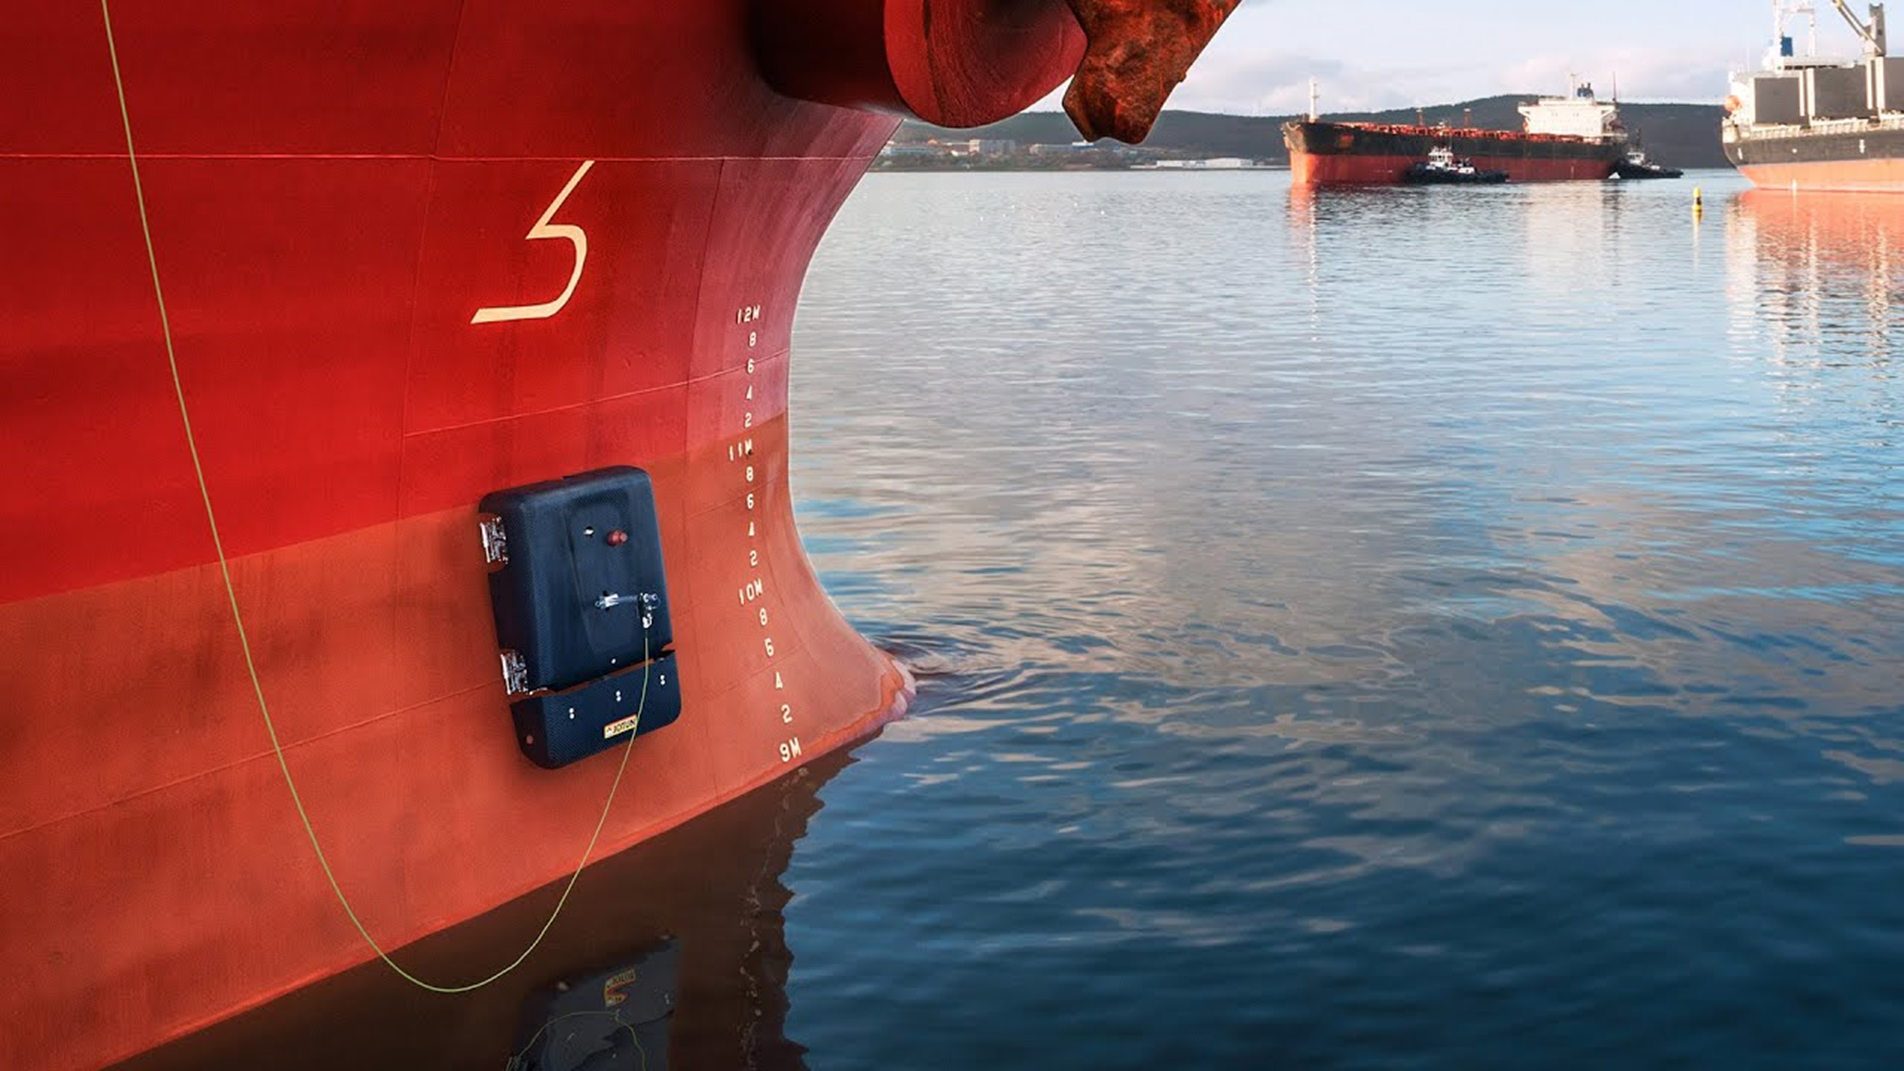
\includegraphics[width=0.7\columnwidth]{figures/hullskater}
    \caption{Hull Skater.}
    \label{fig:hullskater}
\end{figure}

Maritime har kontorer over hele verden, der hovedkontoret ligger i Norge.
HSS, Hull Skating Solutions, er et samarbeidsprosjekt mellom Jotun og Kongsberg Maritime. 
Prosjektet utvikler en robot som kan brukes til å vaske skroget på store skip. 
Dette blir gjort for å hindre uønsket spredning av organismer rundt om i verden, 
samt minke drivstofforbruket på båtene. Slik det gjøres i dag må båtene tas opp på land for å bli vasket, 
eller dykkere må dykke langs skroget for å rengjøre. 
\parencite{Keim2015}


\subsection{Problemstilling}
VeRo ønsker å vite hvor på skipskroget HullSkater befinner seg. Skipskroget er et vertikalt plan 
som står normalt på vannoverflaten. GNSS vil her ikke gi tilstrekkelig presisjon for posisjonen. Noen grunner til dette er:
\begin{itemize}
    \item GNSS gir ikke god høydepresisjon, og vil derfor bli for unøyaktig til dette bruksområdet.
    \item GNSS måler skipets og HullSkater sin posisjon i forhold til jorden.
    \item Skipet vil ikke alltid ligge like dypt i vannet.
    \item GNSS tar ikke høyde for endring i vannhøyden.
\end{itemize}
Med UWB kan man lage et lokalt posisjoneringssystem som vil fikse dette problemet og gi posisjonen til roboten på skroget uavhengig av posisjonen til skipet. 
Mangelen på lokal posisjonering er et problem som oppstår flere plasser hvor det er viktigere å vite posisjonen i forhold til en gjenstand enn plassering på jordens overflate. Eksempler på dette i forbindelse med droneaktivitet er anleggsplasser, maritime operasjoner fra plattform eller skip og inspeksjon av konstruksjoner og bygninger. 
Tidligere er det kun brukt GNSS under disse operasjonstypene. Noen problemer med GNSS i disse situasjonene er:
\begin{itemize}
    \item I forbindelse med operasjoner i urbane miljø er signalrefleksjon et stort problem. Dette gir dårligere nøyaktighet og mindre troverdig posisjon.
    \item GNSS kan lett forstyrres av andre signaler da signalet som treffer jorda er svakt i forhold til andre trådløse former for kommunikasjon.
    \item GNSS har en begrenset evne til å bestemme høyde. På grunn av plasseringen og avstanden til satellittene. 
\end{itemize}

\subsection{Målformulering}
\subsubsection{Formål}
Gruppen skal se på bruken av UWB posisjonering av dronesystemer og se på fordeler og ulemper med dette kontra GNSS.  

\subsubsection{Resultatmål}
Dette prosjektet ønsker å se på bruken av et UWB system på en drone samt å sammenlikne presisjonen med GNSS. For å oppnå dette er det i samarbeid med VeRo satt flere delmål det skal jobbes mot. Disse er laget med økende kompleksitet, da det er vanskelig å si på forhånd hvor mye hvor mye tid det vil ta å oppnå de ulike målene. Målene med UWB er:
\begin{itemize}
    \item Posisjonen til dronen blir loggført under en manuell innendørs flygning.
    \item Dronen holder automatisk posisjonen sin i luften.
    \item Dronen kan lande automatisk.
    \item Dronen kan fly et preprogrammert oppdrag med takeoff, planlagt rute og landing.
\end{itemize}
Det er veldig mange problemer med GNSS-baserte droneoperasjoner som muligens kan løses med UWB-posisjonering. Det er derfor ønskelig å utvikle et system som bruker UWB-posisjonering og undersøke hvilke muligheter med også problemer som dette gir.
Et siste mål er å sammenlikne presisjonen oppimot GNSS. Dette målet regnes som uavhengig i forhold til de andre målene.

\subsubsection{Prosessmål}
Gi studentene erfaring og kompetanse i å samarbeide i team, samt å planlegge og gjennomføre et større prosjekt.

\newpage
\section{Valg av løsning}
Dette kapittelet handler om valg av løsninger for oppgaven. Valg av posisjonssystem for prosjektet er i fokus.

\subsection{Systemkrav}
Systemkrav for valg av posisjonssystem
\begin{itemize}
\item Systemet bør være motstandsdyktig mot interferens
\item Systemet skal ikke interferere andre sendere/mottakere på dronen
\item Posisjon i x/y planet skal være mer nøyaktig enn GNSS (uten RTK), sikter på system med nøyaktighet under 1m.
\item Systemet skal være innenfor regelverk for sendestyrke og frekvenser
\item Systemet skal kunne beregne lokal posisjon 
\item Rekkevidden til systemet bør være over 30meter
\end{itemize}

\subsection{Forslag til andre posisjonsmetoder enn UWB}
Bachelor oppgaven er i samarbeid med bedriften Kongsberg, bedriften har ønsket at prosjektet skal teste UWB som posisjonssystem. Likevel ble andre teknologier vurdert av gruppen for alternative løsninger. System som gir ut posisjon i koordinater ble vurdert og system som finner avstand til objekt slik som lidar og stereokamera ble ikke vurdert. 

\begin{figure}[htp]
    \centering
    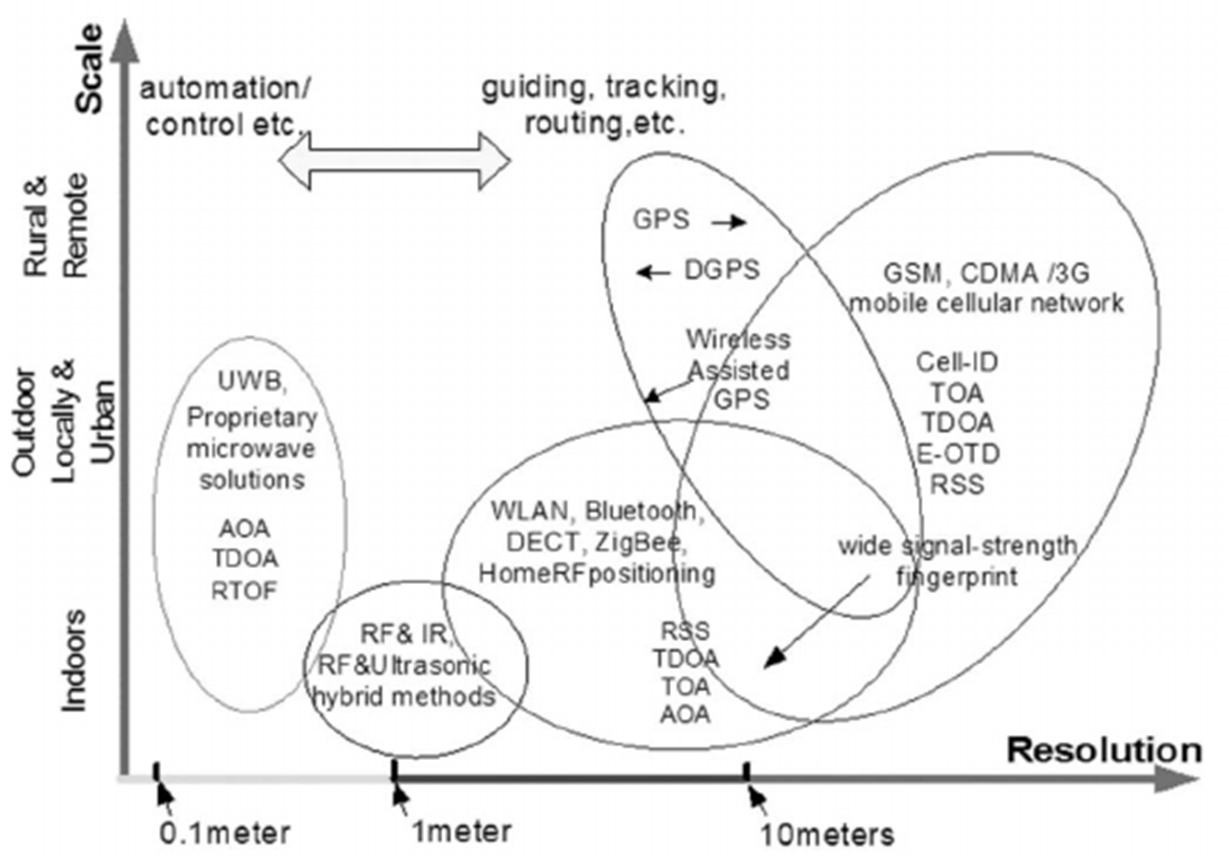
\includegraphics[width=0.7\columnwidth]{figures/posisjoneringssystemer}
    \caption{Sammenlikning av posisjoneringssystemer.}
    \label{fig:posisjoneringssystemer}
\end{figure}

\subsection{Kamera triangulering}

\begin{figure}[htp]
    \centering
    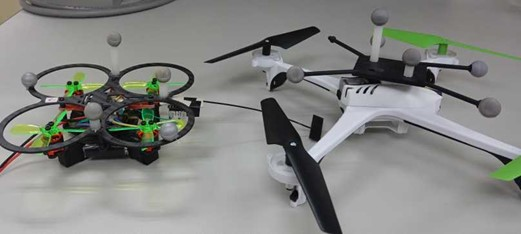
\includegraphics[width=0.7\columnwidth]{figures/kameratriangulering}
    \caption{Droner for kameratriangulering.}
    \label{fig:kameratriangulering}
\end{figure}

Kamera triangulering bruker flere kamera for å triangulere posisjonen til ett eller flere objekt. På objektet som skal spores plasseres flere markører. Slik kan man finne posisjonen og rotasjonen. Denne teknologien er mye brukt i filmproduksjoner og spillutvikling.
Kamera triangulering kan være veldig nøyaktig. Systemet Optitrack beskriver oppløsningsavviket på millimeternivå.  Disse systemene kommer ofte med en høy pris, som er utenfor prosjektets budsjett. Rekkevidden til systemene er og litt kort til prosjektets anvendelsesområde, og utendørsbruk kan være krevende. 

\subsubsection{Bluetooth, Zigbee og Wifi}
Denne teknologien baserer seg på signalstyrke for å beregne posisjonen. Oppløsningen på posisjonen til vil ligger i meterområdet bluetooth (ca 1-5m) og Wifi(ca5-20), det vil være for unøyaktig for prosjektets anvendelsesområde siden det er mer unøyaktig enn GNSS kan være. 
Denne teknologien bruker frekvenser innenfor 2.4ghz og 5.8ghz De fleste droner bruker allerede disse frekvensene for kommunikasjon, her vil sendingen kunne forstyrre hverandre.  

\begin{figure}[htp]
    \centering
    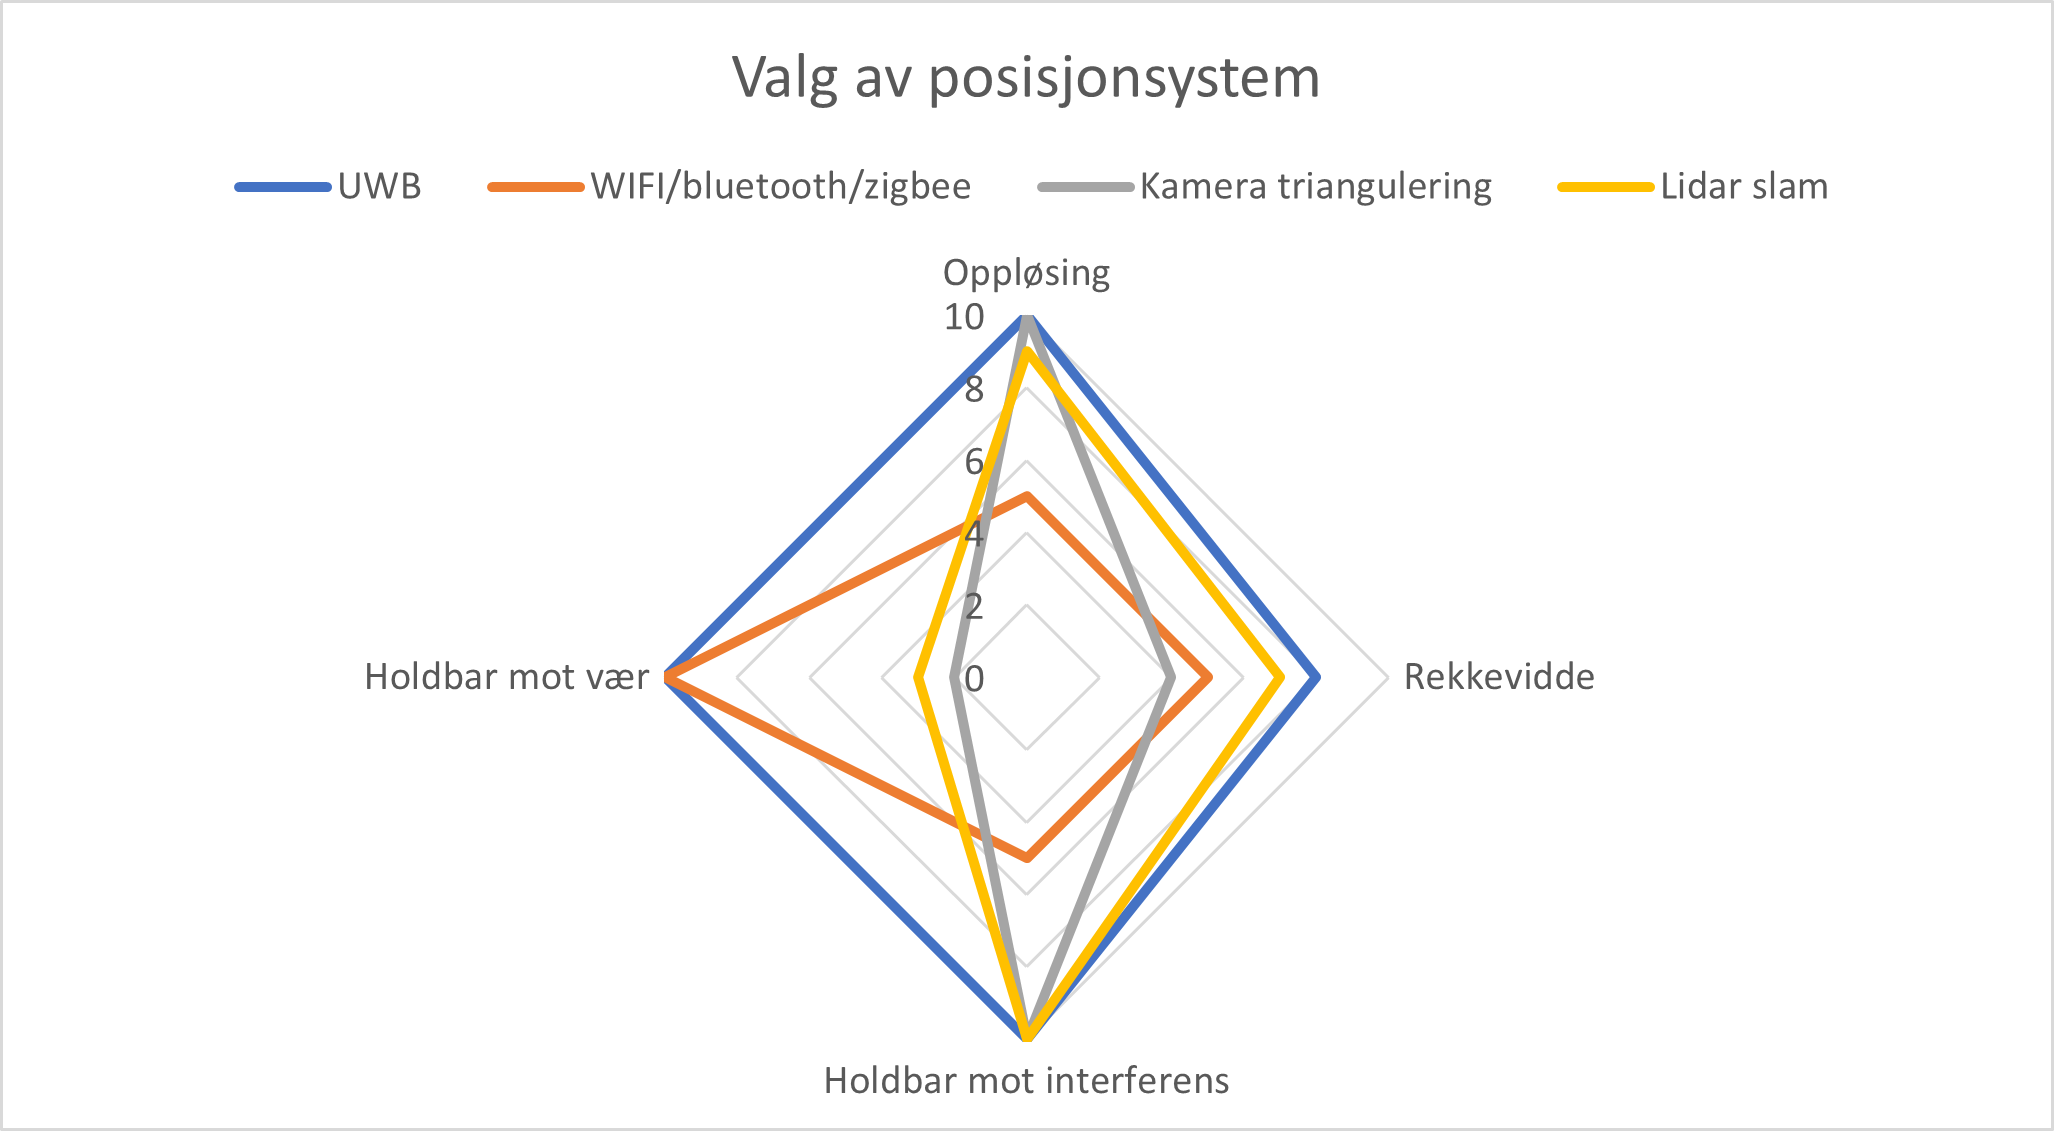
\includegraphics[width=0.7\columnwidth]{figures/valgavsystem}
    \caption{Valg av system.}
    \label{fig:valgavsystem}
\end{figure}

\subsubsection{UWB}
I sammenligningen med de andre posisjonssystemene slår gruppen fast at UWB vil kunne fungere godt for anvendelsesområdet for oppgaven. 

\subsection{Valg av UWB system}
For valg av UWB-system var det 3 forskjellige systemer som ble vurdert.

\subsubsection{DWM100}

\begin{figure}[htp]
\centering
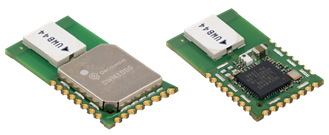
\includegraphics[width=0.5\columnwidth]{figures/dwm100}
\caption{DWM100.}
\label{fig:dwm100}
\end{figure}

Denne UWB modulen består av UWB sensoren DW1000 som er brukt i flertallet av UWB system. For prosjektets bruk sammen med en drone er det nødvendig å lodde modulen til en mikrokontroller. Det trengs og en løsning for å gi strøm til sensorene. 
For å bruke DWM1000 til å finne posisjon er det nødvendig med programvare som triangulerer signalene fra modulene, det finnes ingen tilgjengelig programvare for dette slik at mye arbeid i bacheloren ville gått til programmering. 

\subsubsection{DWM1001}

\begin{figure}[htp]
\centering
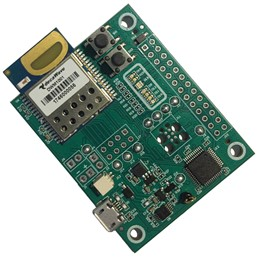
\includegraphics[width=0.4\columnwidth]{figures/dwm1001}
\caption{DWM1001.}
\label{fig:dwm1001}
\end{figure}

DWM1001 består av sensor/mottaker DW1000, i denne modulen er mikrokontroller inkludert, slik det er lite arbeid med oppkobling. 
Slik som DWM1000 vil det være mye arbeid med å programmere systemet til posisjonsbruk. 

\subsubsection{POZYX}

\begin{figure}[htp]
\centering
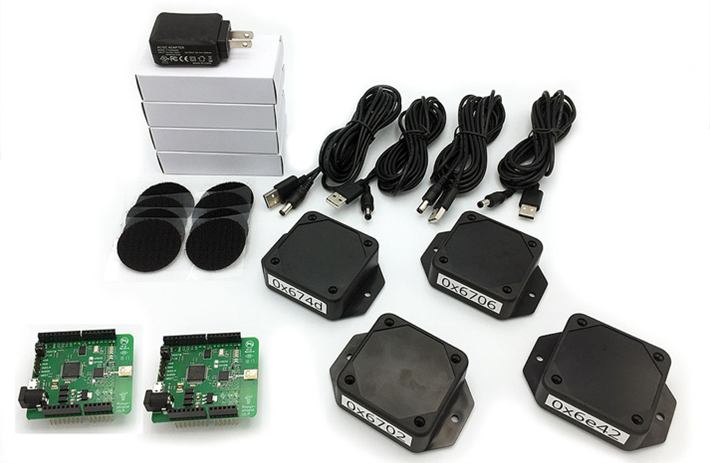
\includegraphics[width=0.7\columnwidth]{figures/creatorkitlite}
\caption{Pozyx creator kit lite.}
\label{fig:creatorkitlite}
\end{figure}

Pozyx systemet består av anker og tags som inneholder mikrobrikken Dw1000.  Creator kit Lite kommer med 4 anker og 2 tags. Dette systemet kommer med programvare og har god dokumentasjon for bruk med egen programvare.   

For å velge hvilket system gruppen skulle bestille ble ulike fakturer vurdert. Figur \ref{fig:valgavsystem2} demonstrerer de ulike faktorene.  Valget falt da på POZYX systemet da det passet godt til vår oppgave, det skal være lett å sette opp og har mye dokumentasjon. 
Det at POZYX systemet har ferdig programvarer og bibliotek passer godt til oppgaven, da oppgaven til prosjektet er ikke å programmere ett UWB-system fra grunnen, men det er å forske på hvordan UWB vil fungere i bruk med droner. 

\begin{figure}[htp]
\centering
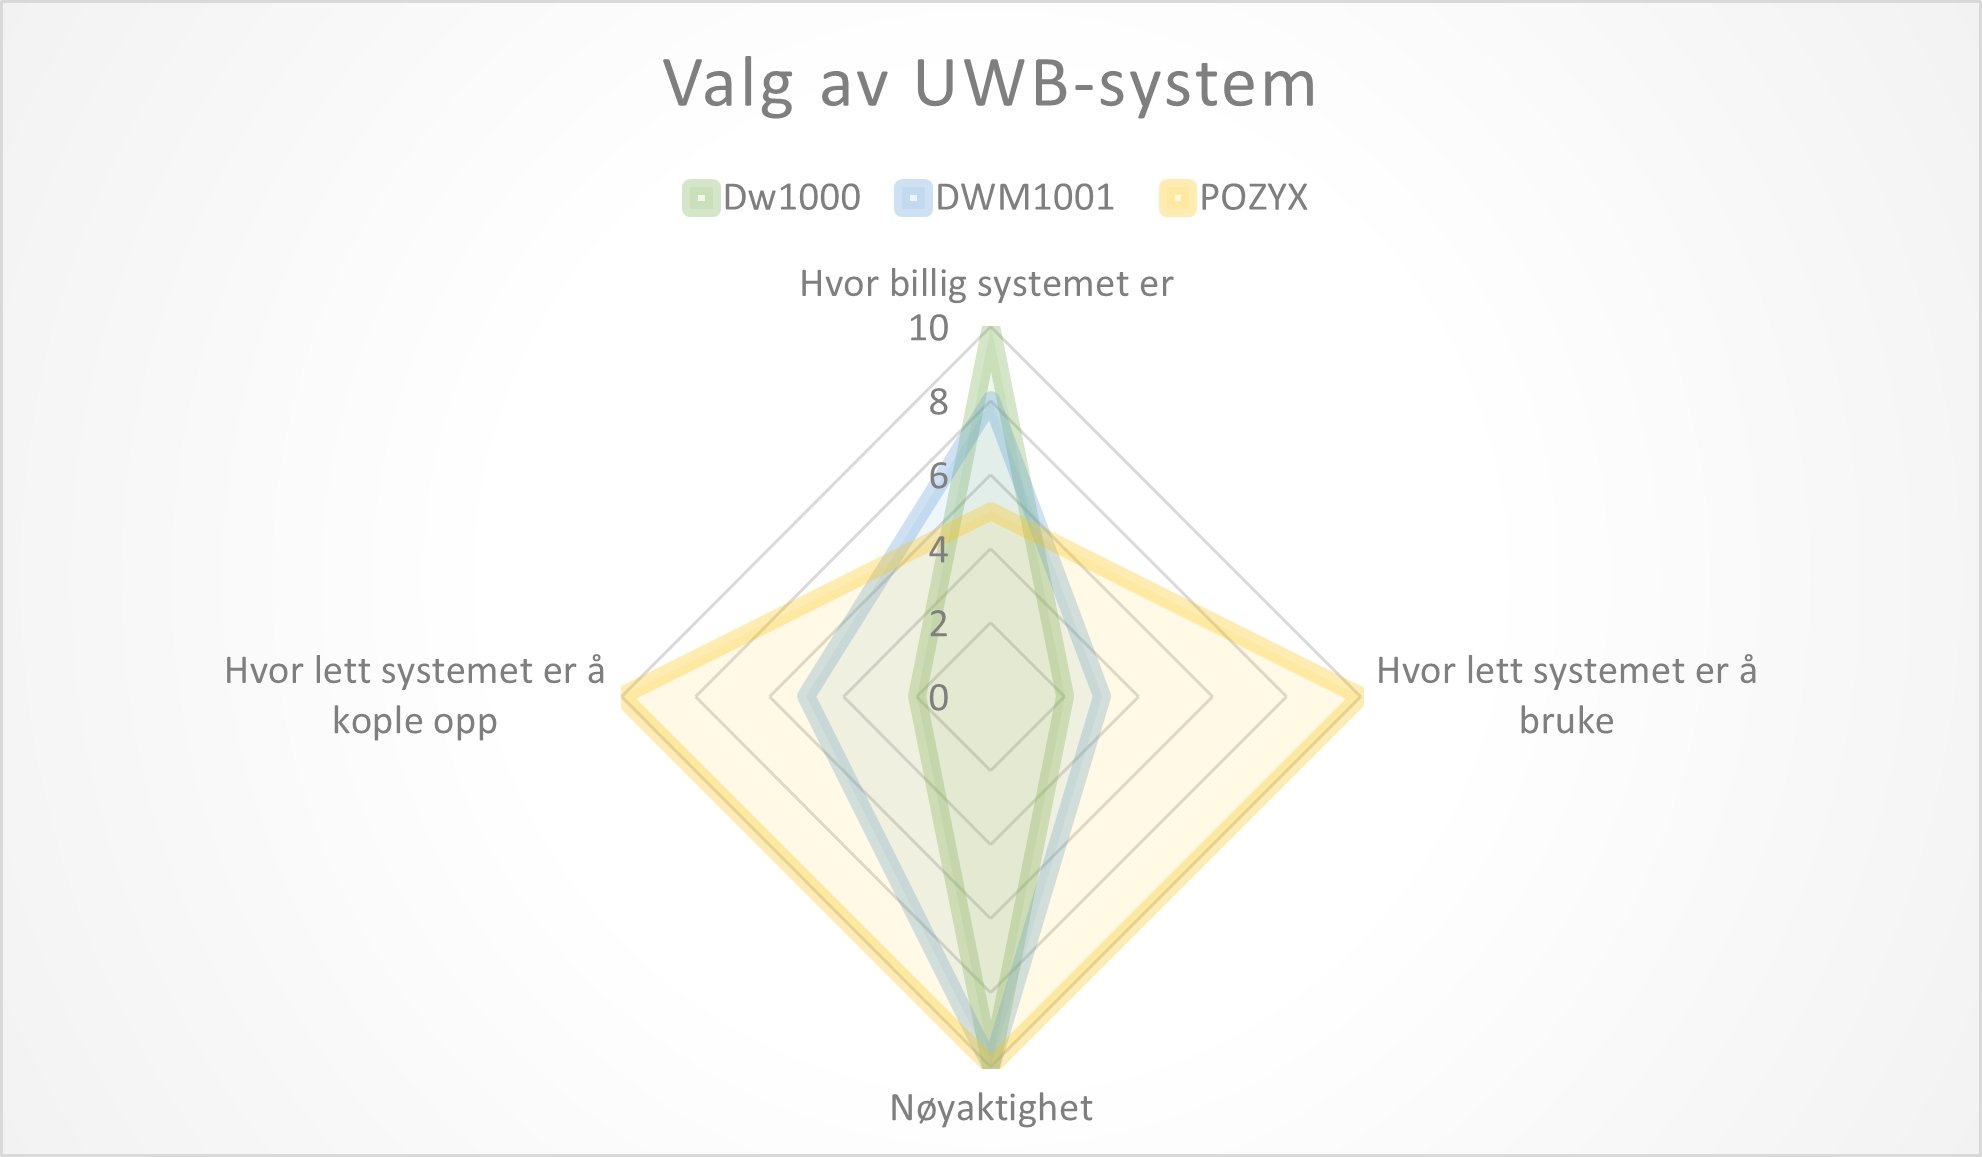
\includegraphics[width=0.7\columnwidth]{figures/valgavsystem2}
\caption{Valg av UWB system.}
\label{fig:valgavsystem2}
\end{figure}

\subsection{Valg av platform}

For å knytte prosjektet opp mot droneteknologiutdanningen har gruppen bestemt seg for å bruke quadrotor (drone) for prosjektet. Om prosjektet fungerer godt med enn drone, vil det sannsynligvis fungere godt for roveren til Kongsberg.
Erfaringer fra utendørsflyvninger i Tromsø der prosjektet utføres er at været er enn stor hindring, det ble derfor valgt å bruke en drone som er mulig å bruke innendørs. Valget ble å bruke en «racing» drone med propellerbeskyttere, som vist i figur \ref{fig:nakeddrone}. Denne dronen har løftekraften til å løfte sensorene som er nødvendig samtidig som den har liten størrelse. 

\begin{figure}[htp]
\centering
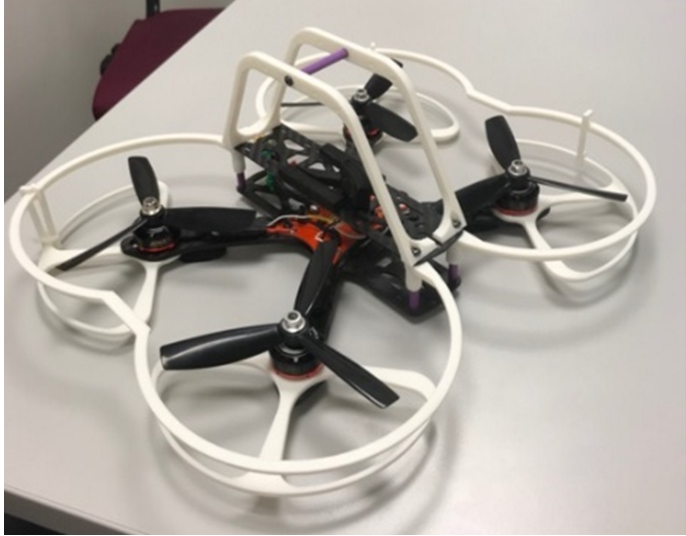
\includegraphics[width=0.6\columnwidth]{figures/nakeddrone}
\caption{Drone ramme med 3D-printet beskyttelse.}
\label{fig:nakeddrone}
\end{figure}

\subsection{Konsept}
Systemet består av et dronesystem med påmontert UWB-tag som kommuniserer med 4 UWB-anker. UWB-tagen regner ut avstandene til ankerene og sender dataen til flightkontrolleren. Målet er å bruke UWB-systemet til å kunne få dronen til å flyve ved hjelp av UWB-posisjon. Figur \ref{fig:konsept} viser dette.

\begin{figure}[htp]
\centering
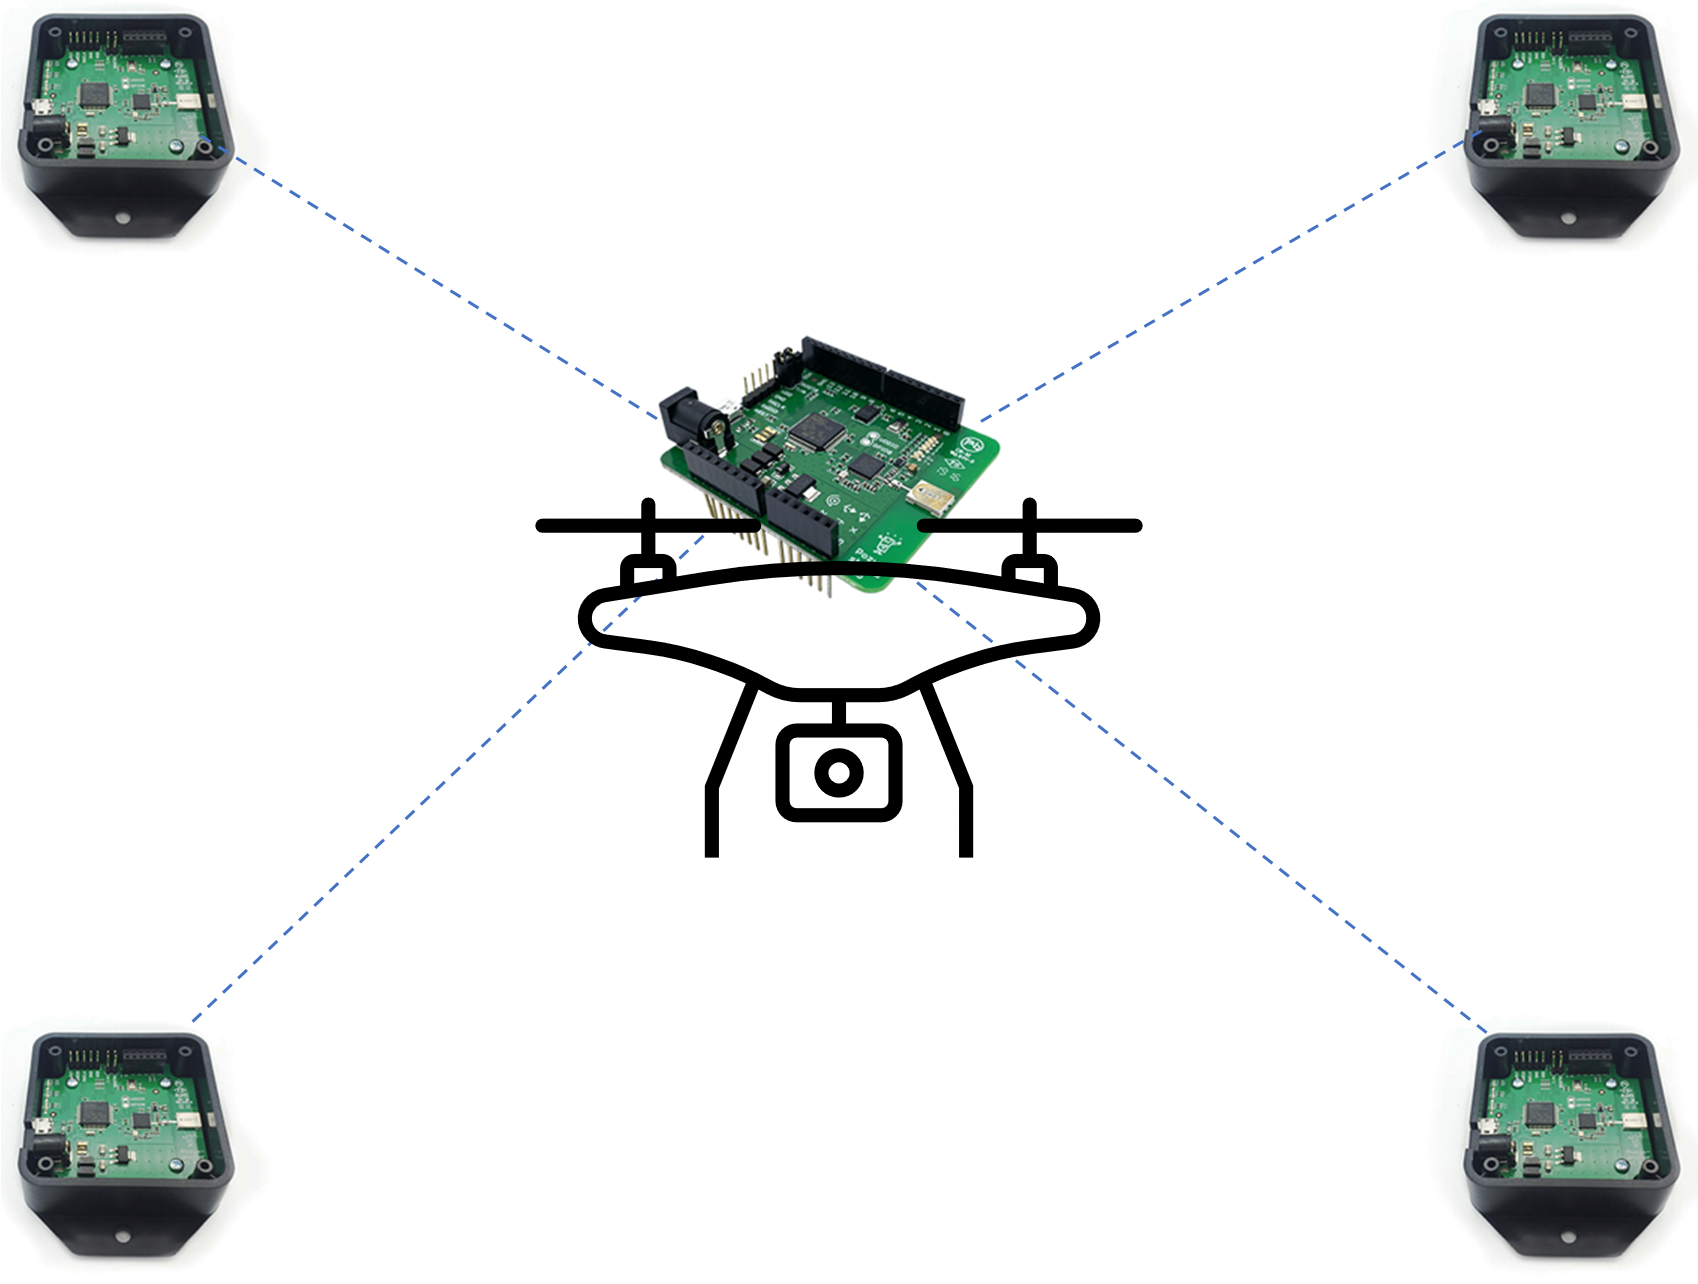
\includegraphics[width=0.5\columnwidth]{figures/konsept}
\caption{Posisjoneringskonsept.}
\label{fig:konsept}
\end{figure}

\subsubsection{Design av drone}
Det ble valgt å bruke en “racing” drone med 5 tommer propeller til prosjektet. For å få den sikker ble det vurdert at propellerbeskyttere måtte bli brukt. 

\subsubsection{3D-printede deler}
Det ble designet propellerbeskytter for å dekke både oversiden og undersiden av propellerbladet. Disse ble deretter festet på drone rammen. For å beskytte UWB-tagen ble det designet ett veltebur på oversiden av dronen. 
Batteriet ble plassert på undersiden av dronen på grunn av UWB-tagen sitter på toppen, for å beskytte batteriet mot harde landinger ble det designet landingsben for å ta imot kreftene. 
De 3d-printede delene ble printet i PLA plast, PLA vil kunne knekke i harde landinger eller krasj, men delene er designet for å kunne bli enkelt byttet ut.  Delene ble designet i Fusion 360. For å finne ut hvor delen vil kunne få svikt ble stressanalyseverktøyet til Fusion 360 brukt, som vist i Figur \ref{fig:stresstest}.

\begin{figure}[htp]
\centering
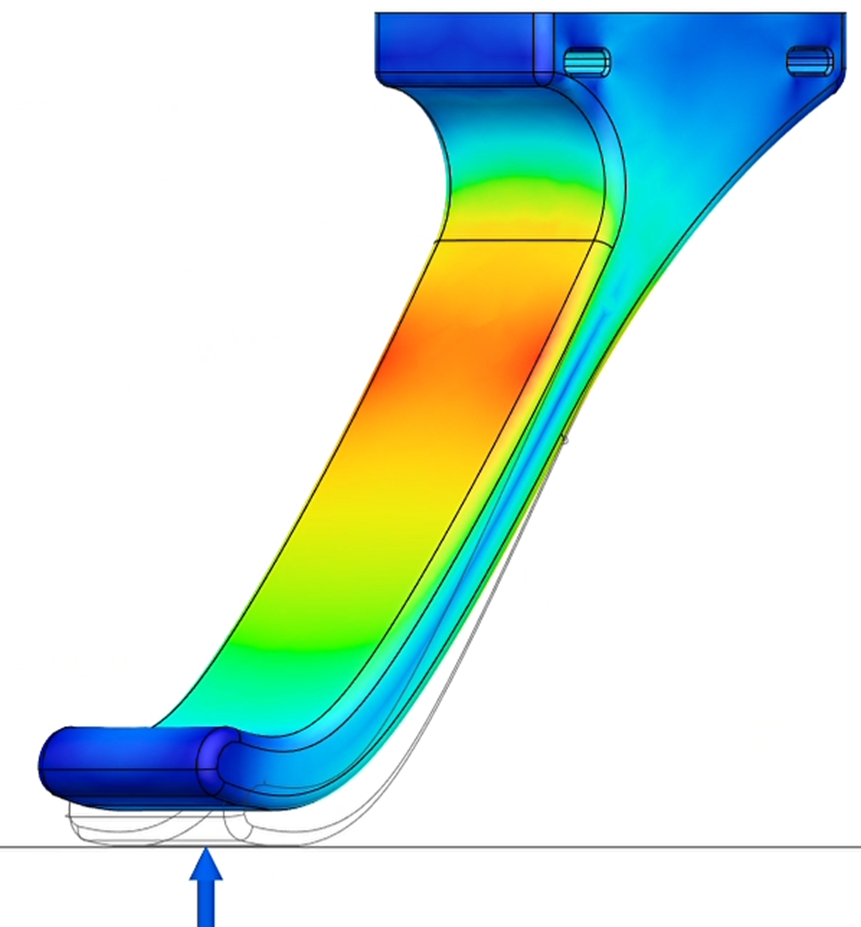
\includegraphics[width=0.4\columnwidth]{figures/stresstest}
\caption{Stresstest i Fusion 360}
\label{fig:stresstest}
\end{figure}

\subsubsection{Oppkobling av dronen}
Dronen består av flightkontroller, motorer, motorkontroller...

\subsubsection{UWB-tag til flightcontroller}
For å få data fra UWB-tagen til rett protokoll til ardupilot var det nødvendig med en mikrokontroller for å “oversette”. I figur\ref{fig:oppkobling} vises oppkoblingen fra UWB-tag t.v til mikrokontroller til flightkontroller. 
På mikrokontrolleren kjøres ett datascript som setter opp UWB-tag for å kunne kommunisere med ankerene ved å sette rette adresser til anker, samt hvor ankerene er plassert. Deretter regnes det ut avstand til hvert anker og koordinat til tag-en. For at flightkontrolleren skal forstå dette må det sendes på riktig protokoll som arduinokoden ordner.   

\begin{figure}[htp]
\centering
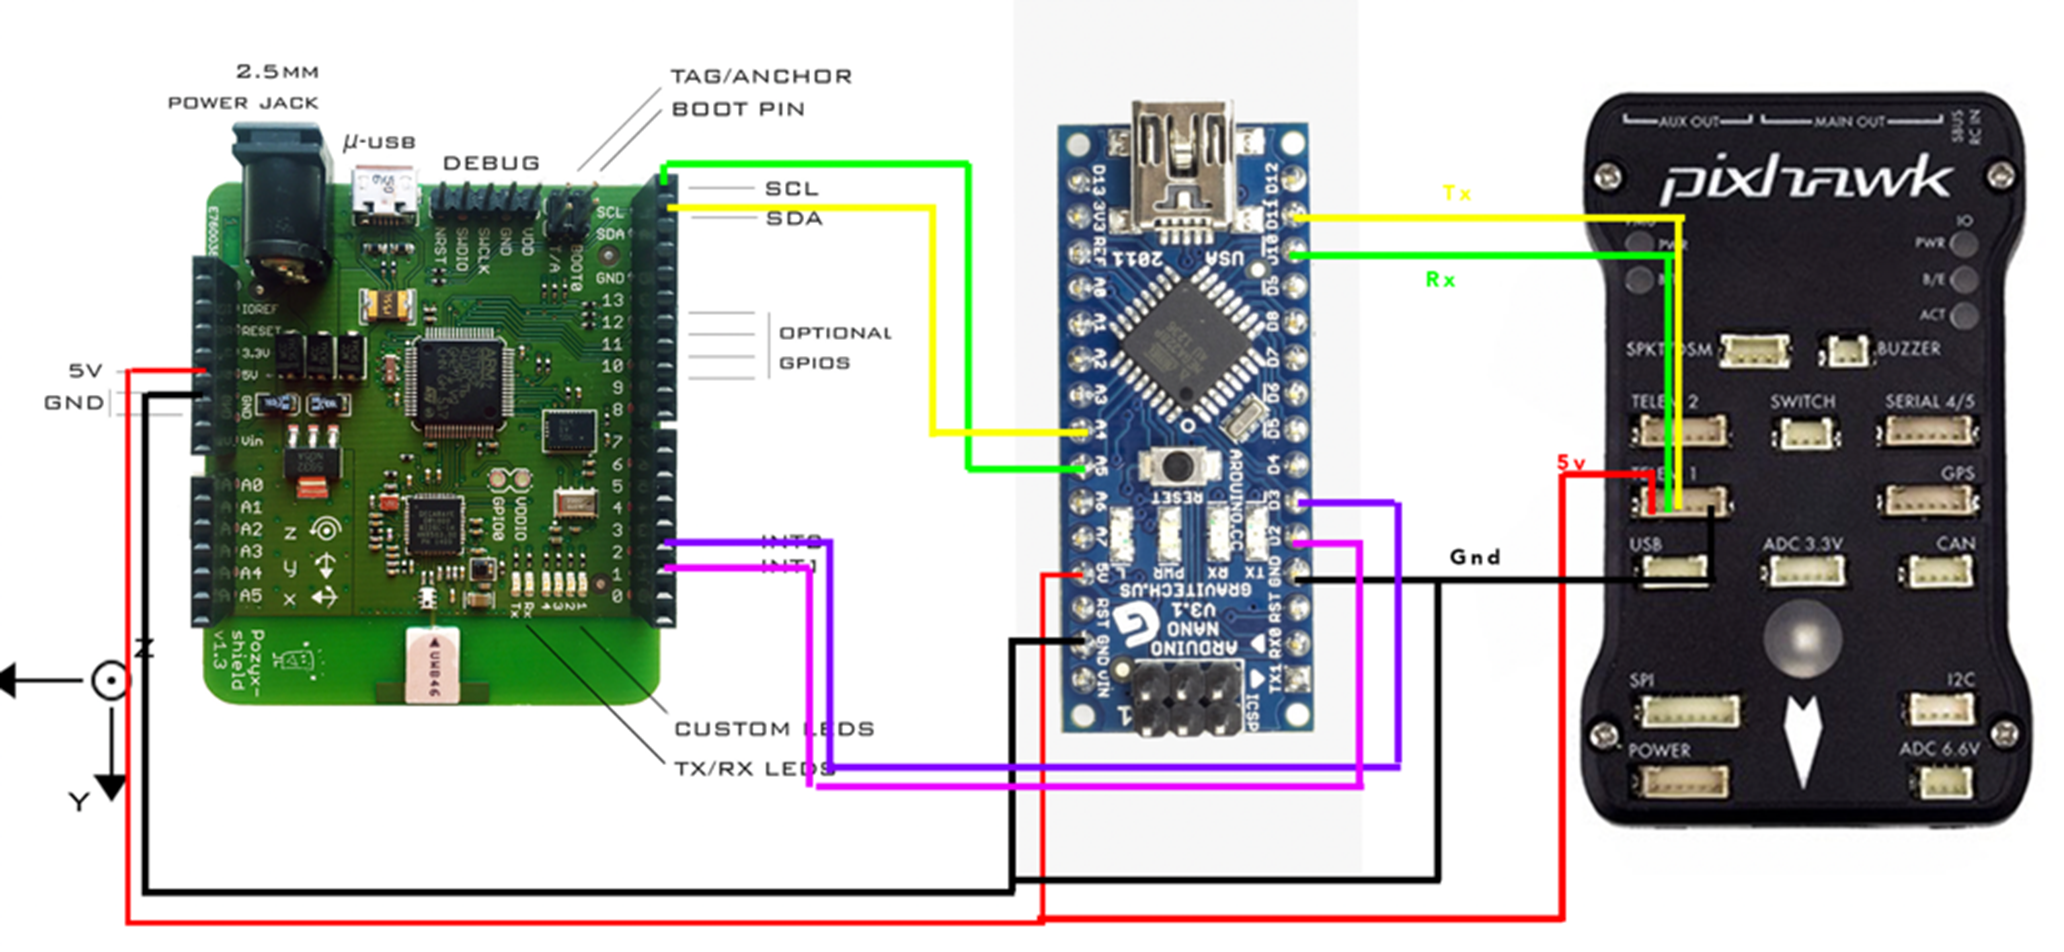
\includegraphics[width=0.7\columnwidth]{figures/oppkobling}
\caption{Oppkobling av "Oversetter" fra UWB-tag til flightkontroller.}
\label{fig:oppkobling}
\end{figure}

\subsubsection{Oppsett av anker}
For at UWB-tag-en skal kunne regne ut posisjonener den avhengign at ankerene er plassert rikig. Det er viktig at ankerene ikke beveger seg, har riktig orientasjon og riktig plasering. Ankerene trenger og strøm for å kjøre siden de svarer tag-en sine meldinger. 
Løsningen her er å bruke borrelås for faste installasjoner, og tripoder for oppsett som er midlertidig.  For å gi ankerene strøm blir små batteripakker brukt, dette bør fungere godt siden ankerene trekke svært lite strøm. 


% Teori
\newpage
\section{Teori}

\subsection{Hvordan finne posisjon}
All posisjonering handler om å finne posisjonen til et objekt i forhold til et annet objekt. 
Den vanligste teknologien for lokalisering på jorden er GNSS (Global Navigation Satelite System), 
ofte bare omtalt som GPS (Global Positioning System). Ved bruk av GNSS kan man finne en posisjon i forhold til jorden, 
altså hvor på jorden man befinner seg. Når UWB brukes til posisjonering opprettes det et LPS (lokalt posisjonerings system). 
Man finner da posisjonen i forhold til dette posisjoneringssystemet, som er nyttig dersom man ønsker å finne posisjonen innendørs der det ikke er GNSS, 
eller ved tilfeller hvor det er viktigere å vite posisjonen i forhold til en konstruksjon enn jorden. Et UWB LPS er satt opp ved bruk av ankere som 
illustrert i figur \ref{fig:ankere}. Et anker velges som origo, og posisjonen til de andre ankerene måles opp i forhold til origo. 
En tag som beveger seg rundt i dette rommet vil kunne bruke ankerene til å regne ut sin egen posisjon. 
Måten dette gjøres på er at tagen først bruker TWR til å finne avstanden til hvert anker. Både disse avstandene og de kjente posisjonene til 
ankrene blir deretter brukt til å regne ut tagens posisjon i forhold til origo.

\begin{figure}[h]
\centering
\subfloat[Ved bruk av et anker kan tagen finne ut hvor langt unna ankeret den er.]{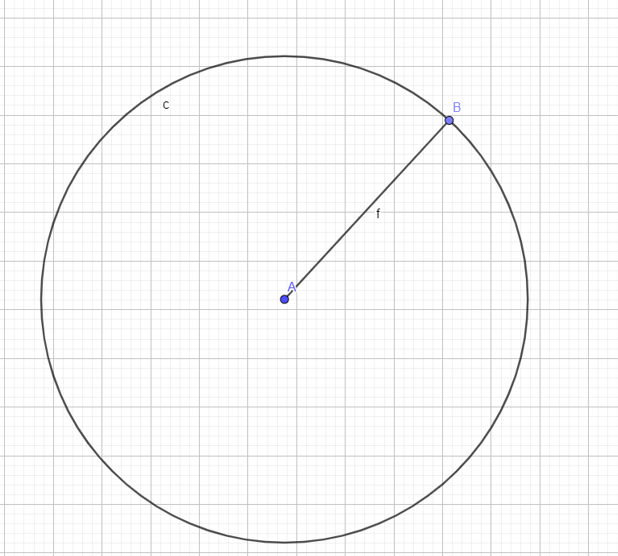
\includegraphics[width=.45\columnwidth]{1anker}} \quad
\subfloat[Ved bruk av to ankere med kjent posisjon kan tagen regne ut to mulige posisjoner den kan være på i 2D.]{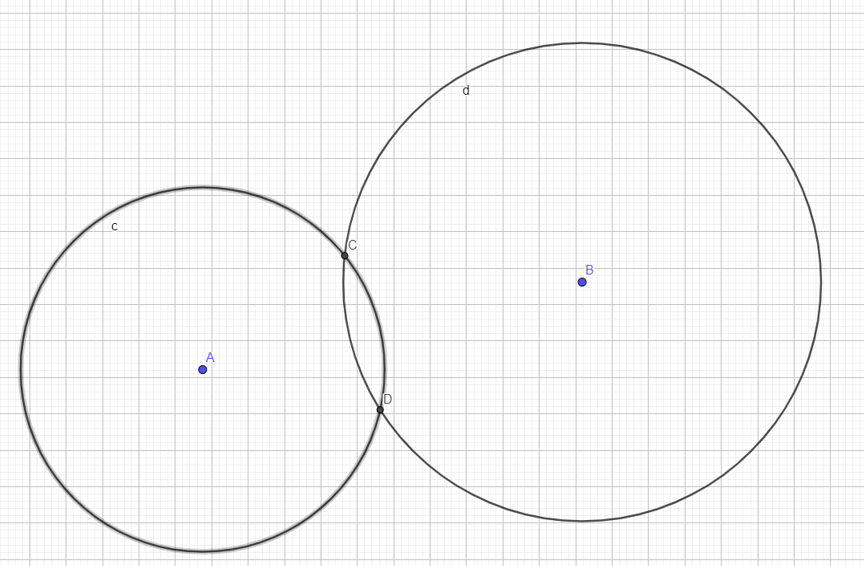
\includegraphics[width=.45\columnwidth]{2anker}\label{fig:ipsum}} \\
\subfloat[Ved bruk av tre ankere med kjent posisjon kan tagen regne ut en absolutt posisjon i 2D.]{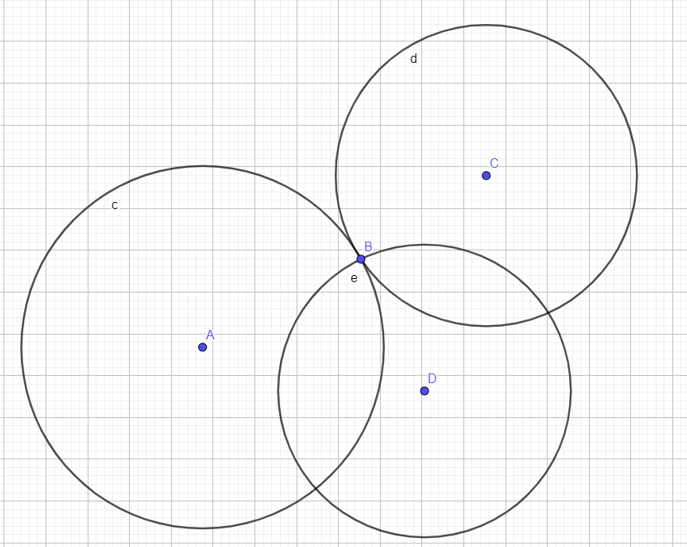
\includegraphics[width=.45\columnwidth]{3anker}} \quad
\subfloat[Ved bruk av 4 eller flere ankere med kjent posisjon kan tagen regne ut en posisjon i 3D, altså i x-retning, y-retning og høyde.]{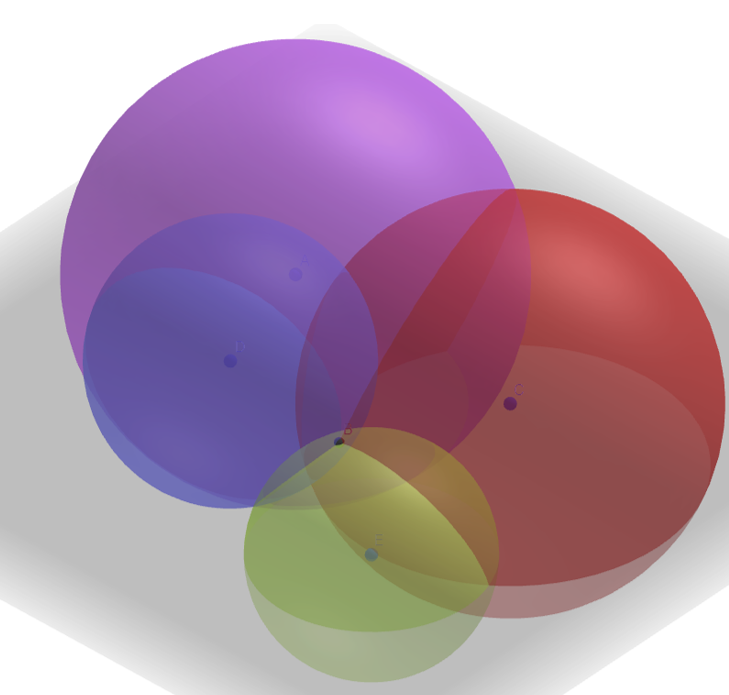
\includegraphics[width=.45\columnwidth]{4anker}}
\caption[Posisjonering ved ulike antall ankere.]{Posisjonering ved ulike antall ankere.} % The text in the square bracket is the caption for the list of figures while the text in the curly brackets is the figure caption
\label{fig:ankere}
\end{figure}

\subsection{UWB}
Ultrabredbånd, eller Ultrawideband (UWB), beskriver radiokommunikasjon med båndbredder høyere enn 500 MHz. 
På slutten av 1900 tallet ble UWB smått tatt i bruk, men ble da mest brukt til radar, sensorer og militært bruk. 
Dette endret seg etter 2002, da US Federal Communication Commission (FCC) vedtok at UWB kunne bli brukt til data kommunikasjon, 
radar og sikkerhets applikasjoner. UWB ble da tildelt frekvensene fra 3.1 til 10.6 GHz, 
som er den største båndbredden til noe kommersielt landbasert system. 
På grunn av at den store båndbredden kunne føre til mye interferens med andre kommunikasjonssystemer, 
ble det satt strenge regler for effekten til UWB. Disse reglene gjør f.eks. at ved bruk av hele UWB spekteret, 7.5GHz, 
vil man ikke kunne bruke en effekt høyere enn 0.5 mW.
Grunnen til at UWB er blitt populært på mange områder er den store båndbredden. Denne gjør at det er mulig å sende mye data med høy frekvens. 
Den lave sende effekten gir både fordel og ulemper. På korte distanser kan man sende mye data samtidig som man bruker veldig lite strøm. 
For å sende data over lengre distanser derimot, trengs mer effekt enn det reglementet for UWB tillater.
\parencite{Mearian2019}

\subsubsection{Two way ranging}

\begin{figure}[htp]
    \centering
    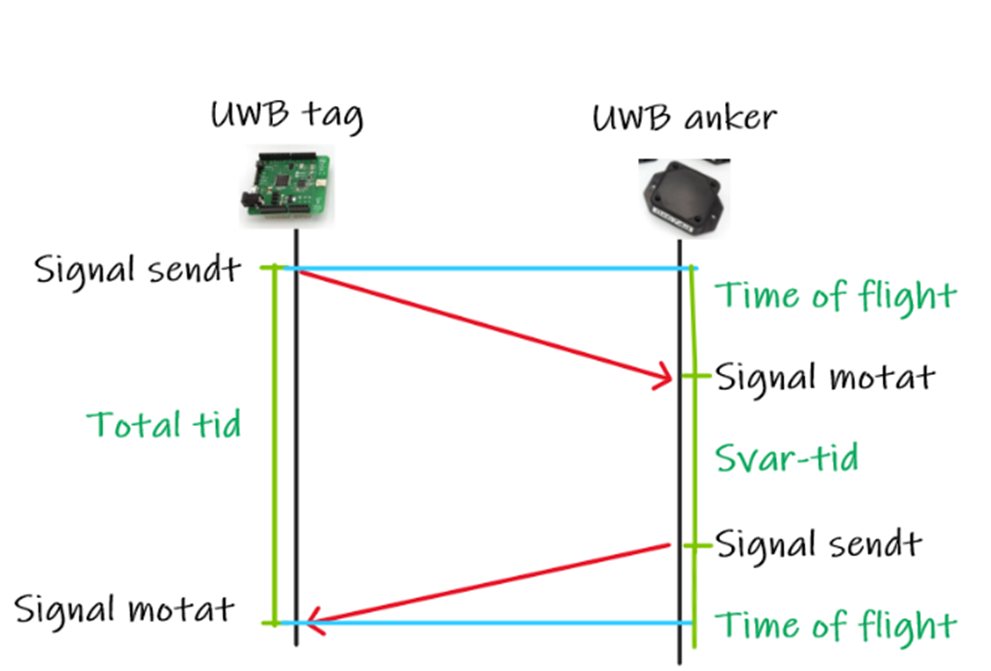
\includegraphics[width=0.7\columnwidth]{figures/twr}
    \caption{Two way ranging.}
    \label{fig:twr}
\end{figure}

For å finne avstanden mellom en tag og et anker brukes two way ranging (TWR) protokollen som vist i figur \ref{fig:twr}. 
Det man er ute etter å finne her er tiden signalet bruker fra ankeret til tagen, og bruke dette til å regne ut avstanden.
Et signal blir først sendt fra tagen til ankeret. Dette signalet bruker tiden $t_{of}$ (time of flight). 
Etter en viss tid, $t_{svar}$, sender ankeret et signal tilbake. Det antas at tiden fra tagen til ankeret er det samme som tiden fra ankeret til tagen, 
altså $t_{of}$. Når tagen mottar signalet tilbake fra ankeret regner den ut tiden fra den sendte ut signalet, 
til den fikk et signal tilbake ($t_{total}$). Dersom $t_{svar}$ er kjent på forhånd, 
kan man regne ut $t_{of}$ er dermed avstanden mellom tagen og ankeret:

\[t_{total} = t_{of} + t_{svar} + t_{of}\]
\[t_{total} = t_{svar} + 2 \cdot t_{of}\]
\[t_of = \frac{t_{total} - t_{svar}}{2}\]

UWB signalet reiser i lysets hastighet, altså: $v_{uwb} \approx 3 \cdot 10^8 m/s$

Dermed kan distansen regnes ut ved:\[d = t_{of} \cdot v_{uwb}\]


Grunnen til at TWR blir brukt er at det ikke krever synkronisering mellom tagen og ankeret. Så lenge $t_{svar}$ er kjent kan distansen regnes ut. 
Denne protokollen gjør også at det er tagen selv som regner ut distansen, 
som gjør det til en god protokoll for bruk på en drone som ønsker å vite sin egen posisjon. 
Det er også mulig å utvide TWR ved at tagen sender ut et ekstra signal etter den har fått signalet tilbake fra ankeret. 
På denne måten kan både tagen og ankeret regne ut avstanden mellom dem.


\subsection{GNSS}
GNSS (Global Navigation Satellite System) er samlebetegnelsen for alle satellittbaserte posisjoneringssystemer som brukes for finne posisjon på 
jordens overflate. Amerikanske NAVSTAR, som var det første operative systemet. Ble fullt utbygd på 1990-tallet og 
var i utgangspunktet tiltenkt militær bruk. Under utviklingen av systemet ble det i tillegg tilgjengelig for det sivile. 
Etter hvert har andre systemer kommet til, slik som GLONASS (Russisk), Galileo (Europeisk) og BeiDou (Kinesisk). \parencite{ForsellGNSS}

\subsubsection{Funksjon}

Felles for alle disse systemene er at avstanden fra en GNSS-mottaker til satellittene brukes til å beregne mottakerens posisjon 
ved hjelp av triangulering. For å triangulere en 2D-posisjon behøves kommunikasjon med tre satellitter, og fire for å kunne definere 
høyden til mottakeren. Jo flere satellittsignaler som benyttes i trianguleringen, jo bedre posisjonsnøyaktighet er det mulig å oppnå. 
\parencite{NorskRomsenter}

Systemene fungerer ved at hver satellitt har et atomur som går svært nøyaktig med neglisjerbare avvik. 
En satellittmottaker har ikke tilsvarende nøyaktig klokke, men mottar jevnlig synkroniseringsdata fra satellittene. 
I tillegg går satellittene i kjente baner, slik at mottakeren på bakken til enhver tid vet hvor satellittene befinner seg. 
Ved å sammenligne tidspunktet signalet ble sendt med tidspunktet signalet ble mottatt, 
kan systemet beregne avstanden til mottakere ved hjelp av «time of flight»-beregning vist i figur \ref{fig:code-positioning}. 
Denne beregningen kan gjøres på flere måter, som igjen vil kunne gi forskjellig nøyaktighet i posisjoneringen. \parencite{ForsellGNSS} 

\begin{figure}[htp]
    \centering
    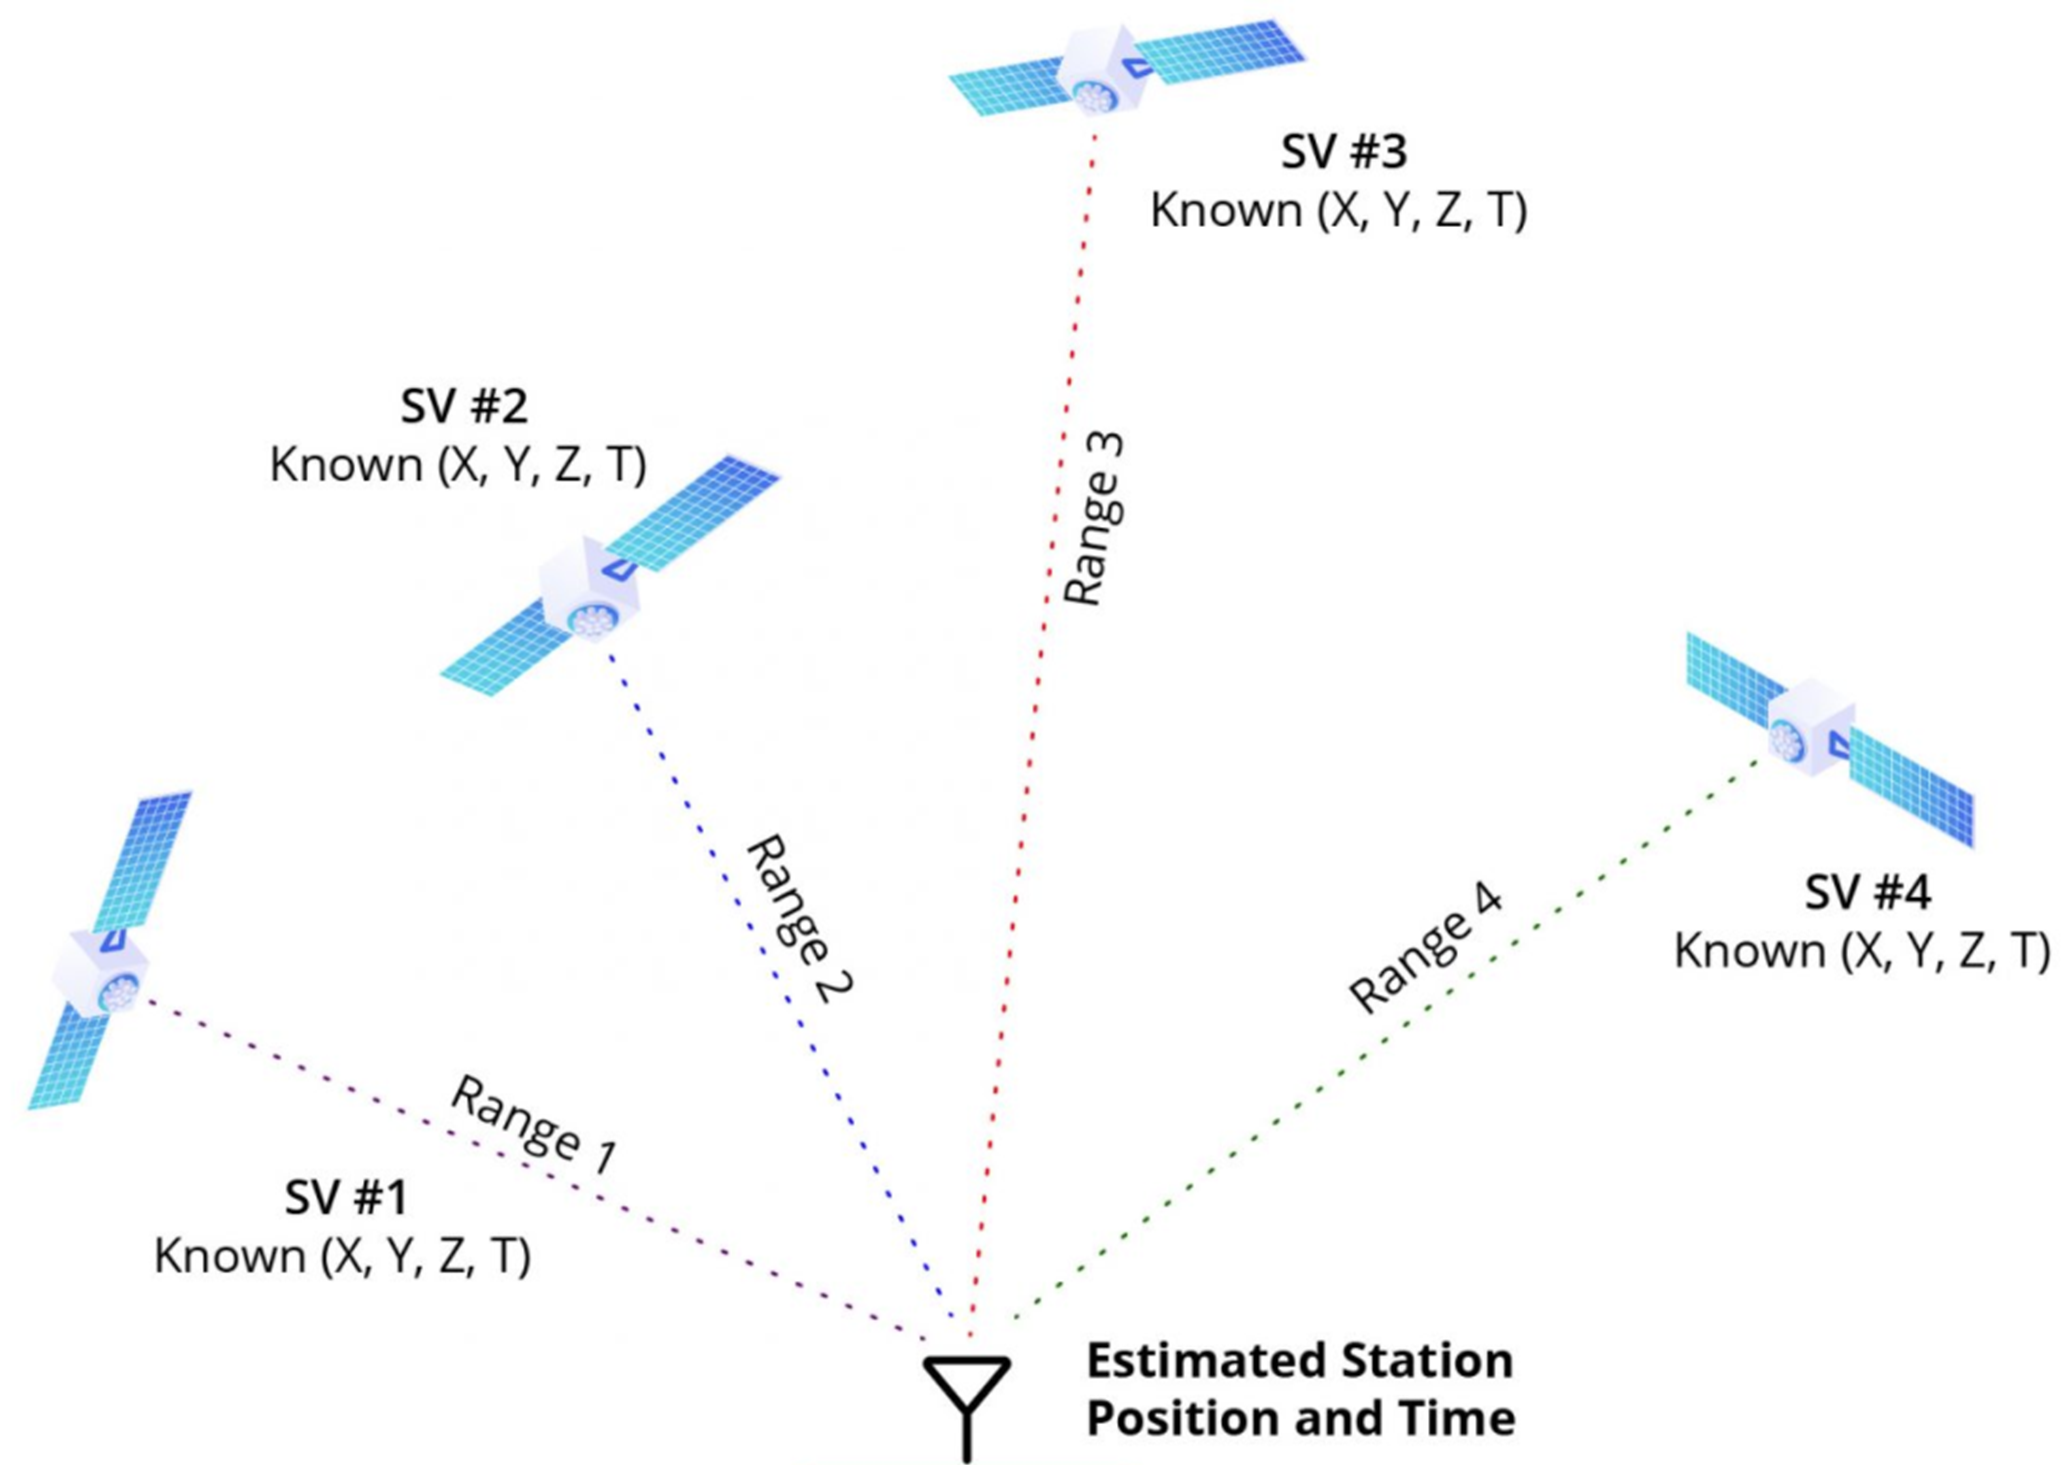
\includegraphics[width=1\columnwidth]{figures/code-positioning}
    \caption{Code-positioning. \parencite{Tallysman}}
    \label{fig:code-positioning}
\end{figure}

Teoretisk sett kan nøyaktigheten i avstandsbestemmelsen fra en GNSS-mottaker til en GNSS-satellitt være omkring 1 meter for den 
enkleste formen for avstandsberegning (beregnet ut ifra det amerikanske systemet). Videre kan mer avanserte metoder som 
fasemåling gjøre at den teoretiske nøyaktigheten kommer ned mot millimeternøyaktighet da bølgelengden til bærefrekvensen L1 er på 19 cm. 
Fasene er periodiske og derfor kan ikke fasemåling brukes alene, da dette vil gi mange mulige avstander til satellittene. 
En tredje metode er differensiell måling, hvor en basestasjon ved et fastpunkt med kjent posisjon måler avvik mellom 
målt posisjon og faktisk posisjon. Dette avviket sendes så til en GNSS-sensor i nærheten som benytter avviket til å beregne 
en svært nøyaktig posisjon. Jo nærmere GNSS-sensoren er fastpunktet, jo mer korrekt er avviksdataen og dermed blir den målte 
posisjonen mer korrekt. \parencite{ForsellGNSS}

\subsubsection{Nøyaktighet}
I bruk kan man ikke forvente å oppnå den teoretiske nøyaktigheten, da det er svært mange feilkilder som påvirker posisjoneringen. 
For å estimere hvor nøyaktig systemene faktisk er så benytter man begrepet «User Range Error» (URE) fra satellitten. 
I 1990 var URE omkring 4.6 meter, og i 2019 var gjennomsnittlig URE nede på cirka 0,5 meter. \parencite{ForsellGNSS}

\subsubsection{Feilkilder}

\begin{figure}[htp]
    \centering
    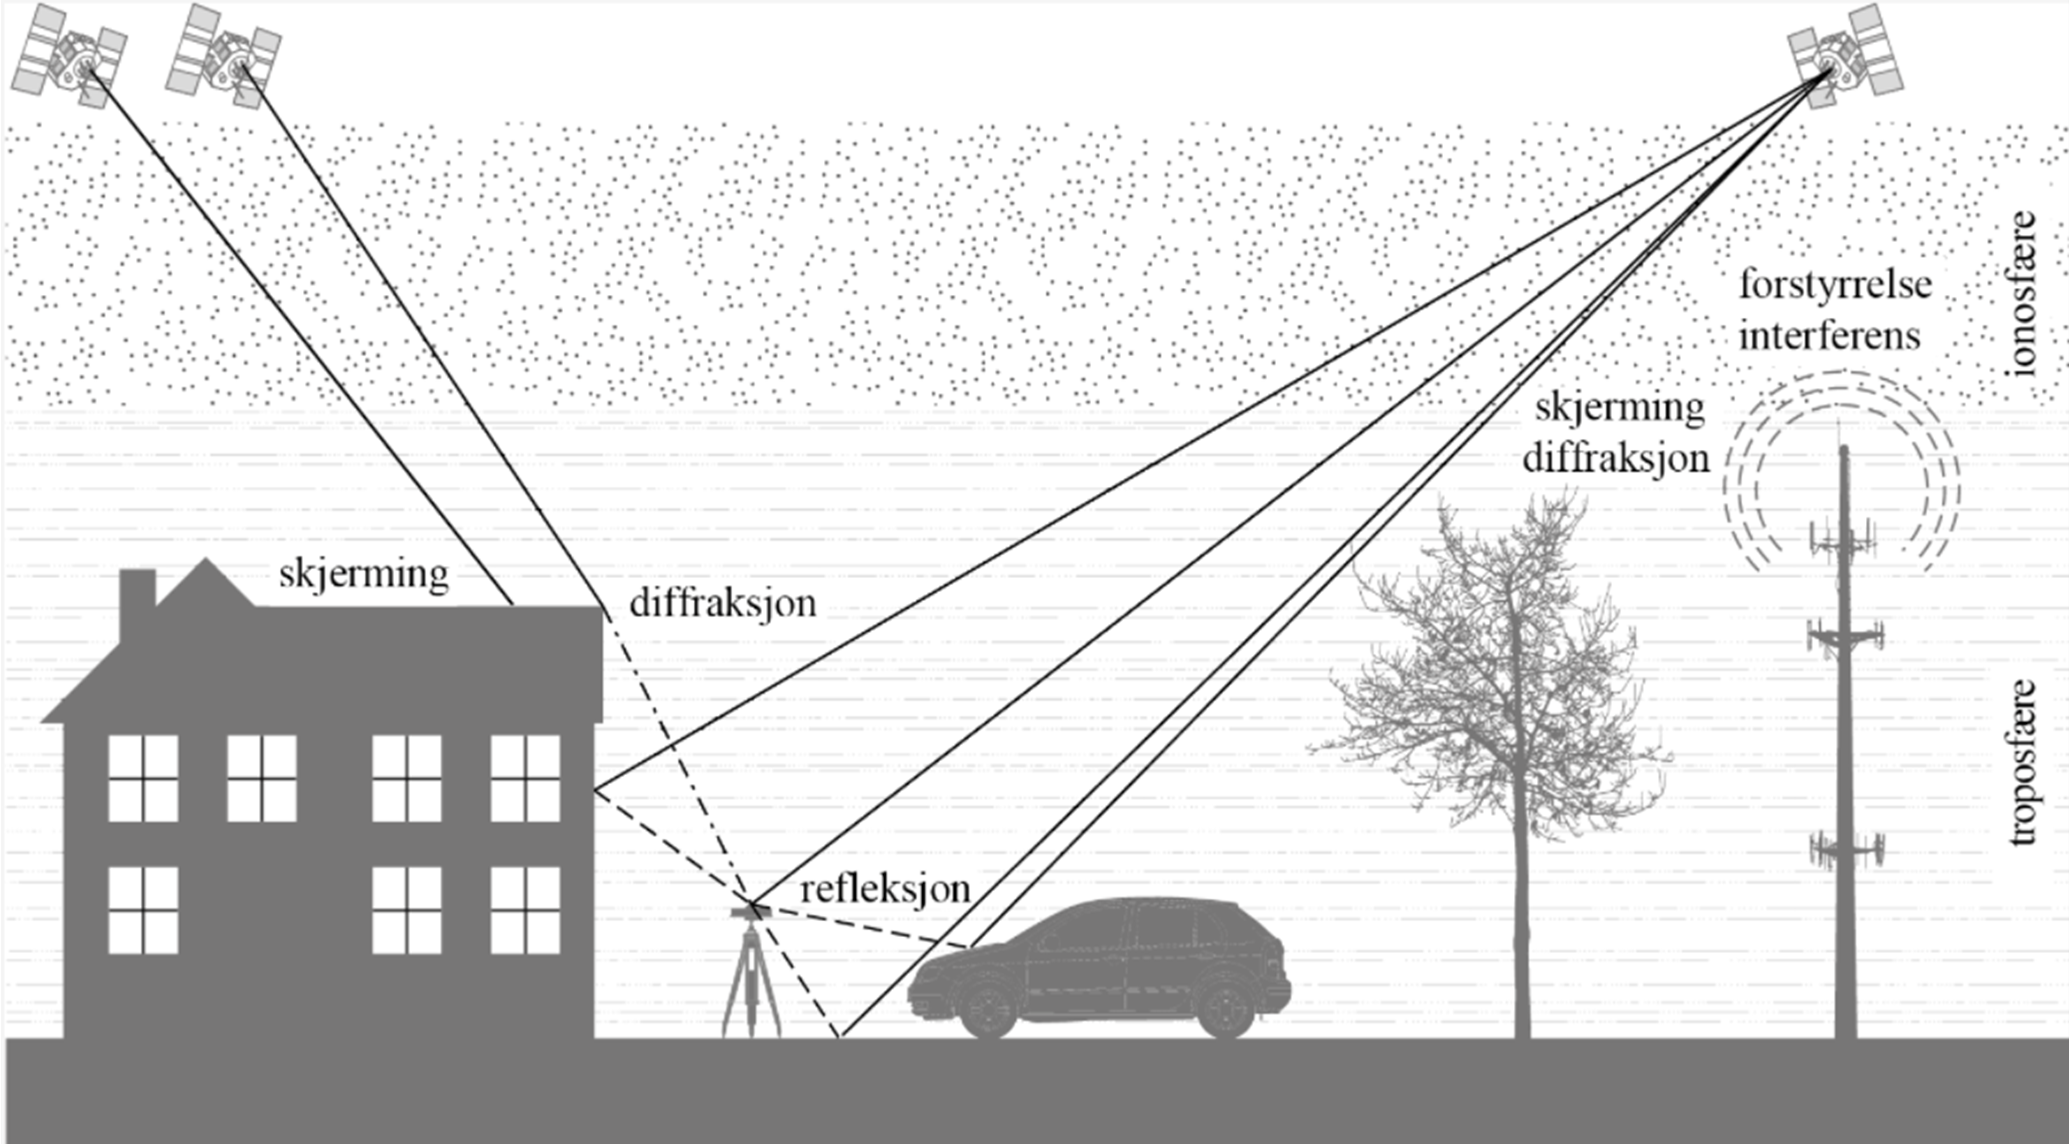
\includegraphics[width=1\columnwidth]{figures/gnss-feilkilder}
    \caption{GNSS-feilkilder.\parencite{NorskRomsenter}}
    \label{fig:gnss-feilkilder}
\end{figure}

GNSS utsettes for en rekke feilkilder som gjør at det er vanskelig å oppnå den teoretisk mulige nøyaktigheten. 
Figur \ref{fig:gnss-feilkilder} illustrerer de forskjellige feilkildene GNSS er utsatt for.

\begin{itemize}
\item Det kan oppstå feil i banedataen til satellittene. Dette kan komme av teknisk feil, eller at det er lenge siden banedataen er oppdatert. Dette vil føre til at GNSS-mottakeren beregner sin posisjon basert på feil posisjon på satellittene.
\item Signalene fra satellittene går i lysets hastighet, men de forsinkes noe gjennom atmosfæren, hvor blant annet luft bremser hastigheten. Hvis lokale forhold gjør at signalene forsinkes mer enn vanlig kan dette fremtvinge flere meter avvik i posisjon.
\item Hvis mottakeren ikke har klar sikt i alle himmelretninger, kan dette dekke for satellitter. Dette kan gjøre at posisjonen beregnes med færre satellitter enn ønskelig. Noe som fører til lavere nøyaktighet.
\item GNSS-signalene har svært lav effekt, og vil derfor lett kunne forstyrres av lokale signaler i nærheten av mottakeren som oppleves sterkere og som bruker omtrentlig lik frekvens som GNSS.
\item GNSS-signalene har en liten, men ikke neglisjerbar evne til å bøye seg rundt hindringer. Dette kan føre til at en mottaker som egentlig er skjult for en satellitt mottar signaler likevel. Disse signalene vil avvike fra den faktiske distansen til satellitten.
\item Signalene har lett for å reflektere fra overflater og gi falske forsinkede signaler til mottakeren. Dette er vanlig i urbane områder hvor det er mange blanke og flate overflater som kan reflektere signalene. Det kan også forekomme i naturen i nærheten av fjell og vann som har reflekterende egenskaper. \parencite{NorskRomsenter} 
\end{itemize}

I tillegg til disse feilkildene vil satellittenes posisjon i forhold til hverandre påvirke nøyaktigheten. 
Hvis en mottaker benytter satellitter som ligger svært tett eller på rekke, vil nøyaktigheten påvirkes negativt. 
Det er fordelaktig med satellitter med god spredning slik at vinklene mellom dem blir størst mulig. 
Dette gjør at krysningspunktene mellom radiene til hver satellitt blir minst mulig. \parencite{NorskRomsenter}

\subsection{Arduino}
Arduino er en opensource plattform som inneholder både Arduino brett og Arduino kodespråk (basert på Wiring). 
Arduinoen brukt i dette prosjektet er en Arduino Nano (figur \ref{fig:arduino-nano}), som er basert på mikrokontrolleren ATmega328. 
Koden skrives i Arduino sin egen IDE, som også brukes til å laste opp kode og monitorere data fra Arduinoen. \parencite{ArduinoNano} 
I dette prosjektet blir Arduinoen brukt som en adapter mellom Pozyx tagen og Pixhawk flightcontrolleren. 
Den leser av avstandene til ankrene fra tagen, og sender denne informasjonen til pixhawken via MavLink.

\begin{figure}[htp]
    \centering
    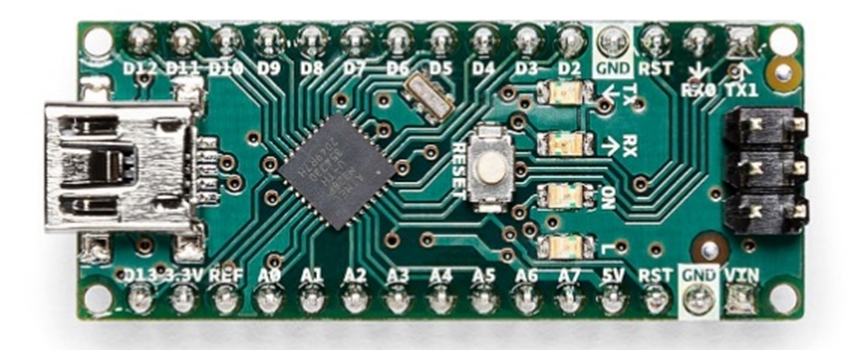
\includegraphics[width=0.5\columnwidth]{figures/arduino-nano}
    \caption{Arduino nano.\parencite{ArduinoIntroduction}}
    \label{fig:arduino-nano}
\end{figure}
    

\subsection{Elektronisk kompass/magnetometer}
Et magnetometer er et instrument som benyttes for å måle styrken og retningen på det magnetiske feltet som virker på instrumentet. 
Dette kan gjøres på flere måter. De to vanligste typene benytter Hall-effekt eller magnetoresistans for å måle magnetfeltet. \parencite{Skaar2021} 

\subsubsection{Hall-effekt}
Hall-effekten går ut på at ladde partikler i en leder vil trekke mot en av sidene i lederen dersom de blir utsatt for et magnetfelt. 
På grunn av et overskudd av ladde partikler på den ene siden oppstår det en spenningsforskjell på tvers av lederen som 
kan brukes til å måle magnetfelt. Hall-effekten er en utvidelse av Lorentz kraften, som beskriver kraften som påføres en 
ladd partikkel som går gjennom et magnetfelt. Hvis magnetfeltet er orientert vinkelrett på retningen av partikkelens bevegelse, 
vil partikkelen oppleve en kraft som er vinkelrett på både bevegelsesretningen og orienteringen av det magnetiske feltet. \parencite{Keim2015}

\begin{figure}[htp]
\centering
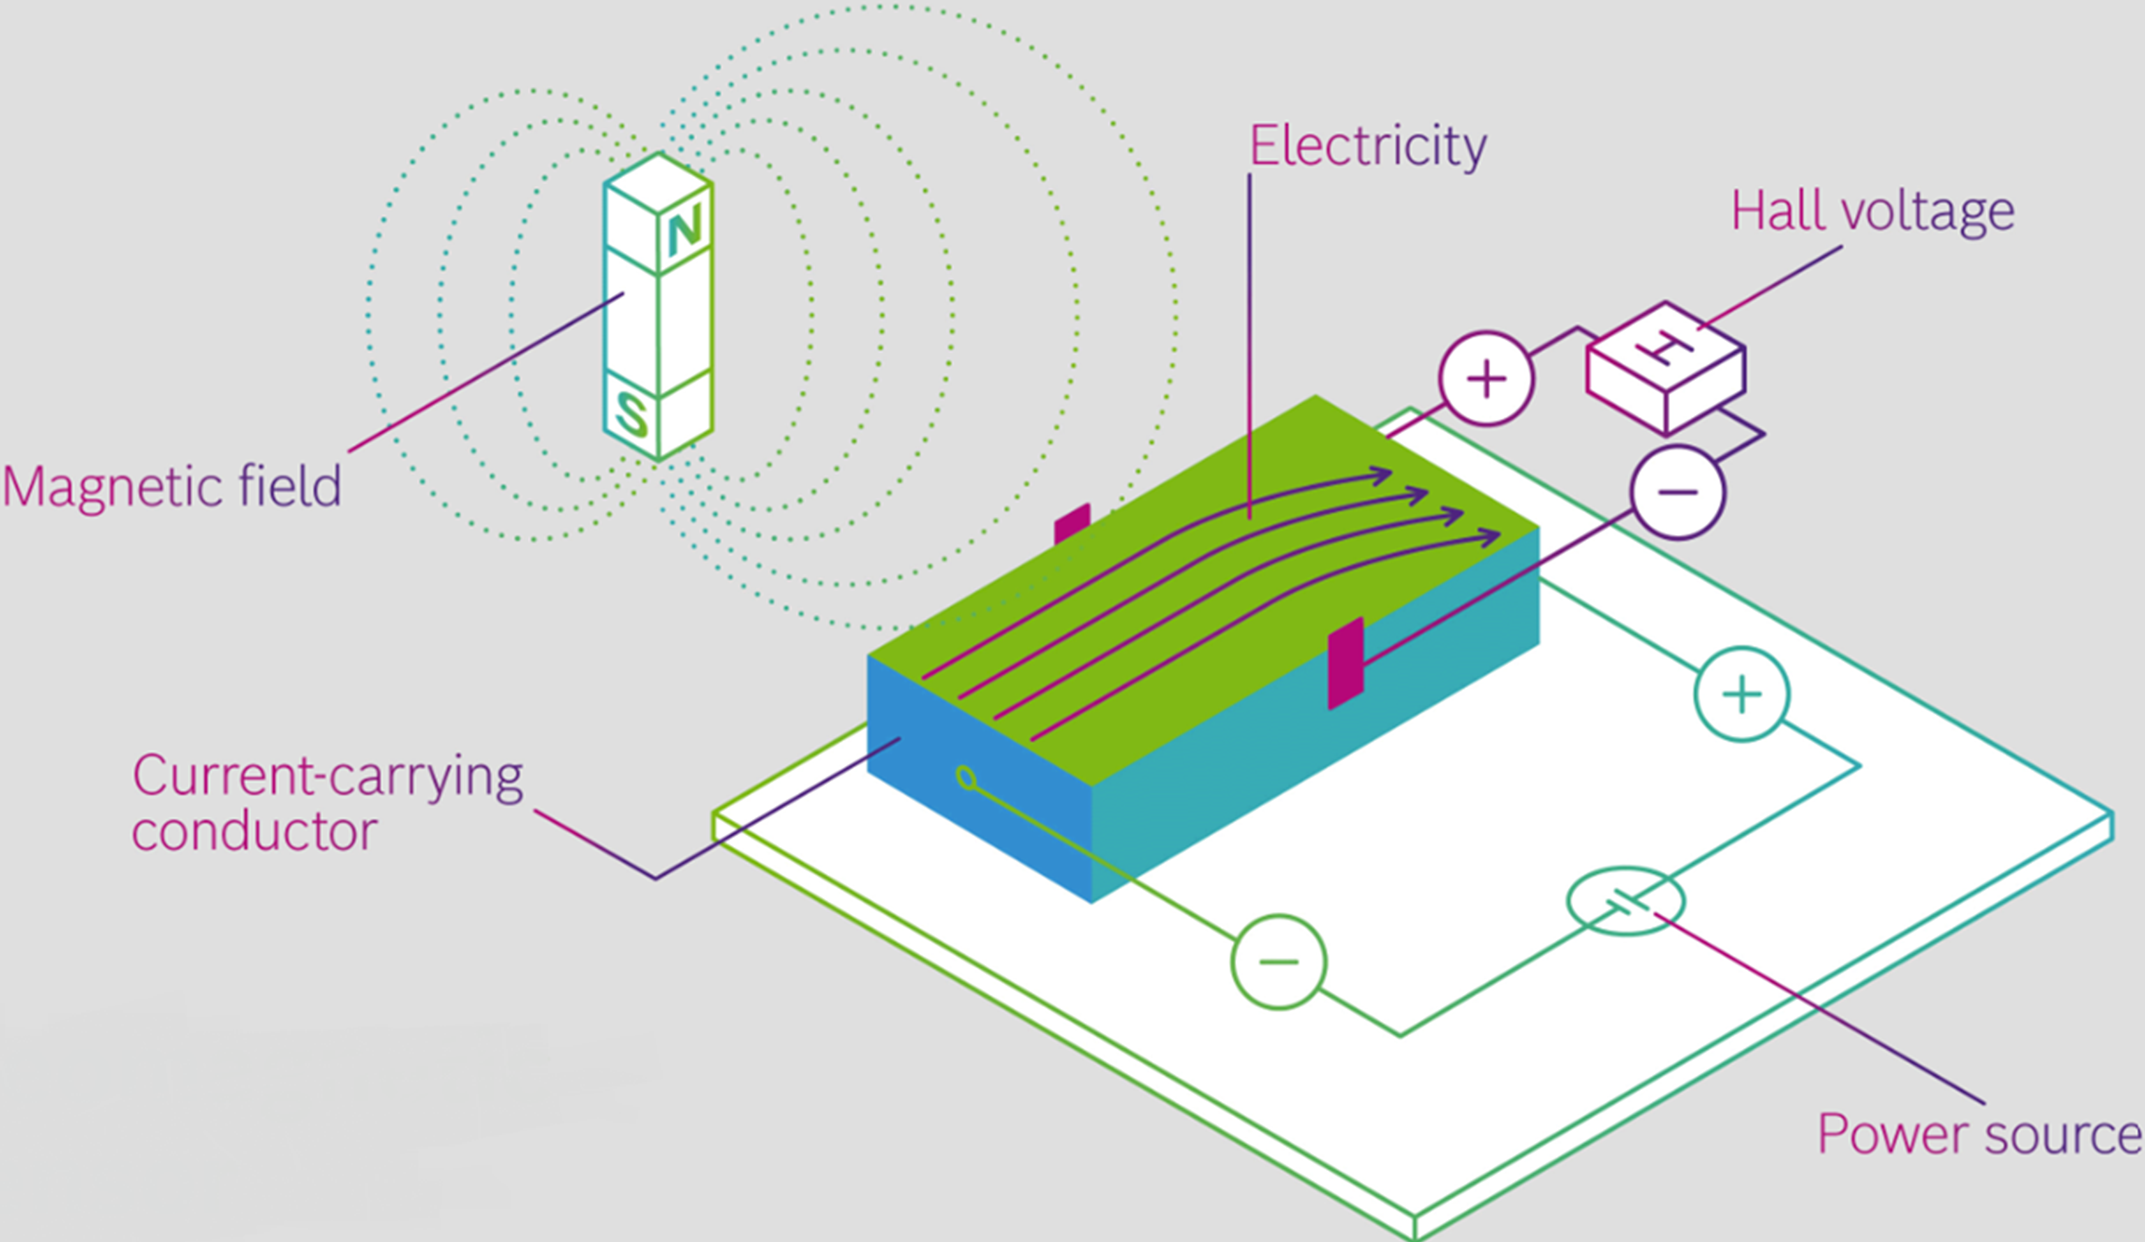
\includegraphics[width=0.5\columnwidth]{figures/hall-sensor}
\caption{Hall-sensor. \parencite{Bosch}}
\label{fig:hall-sensor}
\end{figure}

En Hall-sensor er i sin enkleste form et voltmeter som måler spenningen på tvers av en leder. 
Et magnetometer basert på Hall-effekten benytter typisk to eller flere Hall-sensorer for å kunne 
detektere magnetfelt i et plan eller tredimensjonalt. Dette gjøres ved at sensorene orienteres slik 
at hver sensor måler i hver sin akse, x-y-z. 

\subsubsection{Magnetoresistans}
Magnetoresistans (MR) er en effekt som oppstår når enkelte ledere og halvledere utsettes for et magnetisk felt. 
Alle metaller har en form for MR, men styrken varierer fra metall til metall. 
Effekten går ut på at det oppstår en endring i et metalls elektriske-motstand når et magnetisk felt påvirker metallet. 
Et MR-kompass vil i likhet med Hall-kompass benytte flere sensorer for å nøyaktig måle retningen til jordens magnetiske felt.
MR skiller seg fra Hall-effekt ved at den måler parallelle magnetfelt i motsetning til vinkelrette magnetfelt. 
Dette gjør at en MR-sensor vil oppnå et større deteksjonsfelt. 
I tillegg har en MR-sensor høyere sensitivitet og lavere strømforbruk enn en Hall-sensor. \parencite{ROHM}

\subsubsection{Magnetfelt}

\begin{figure}[htp]
\centering
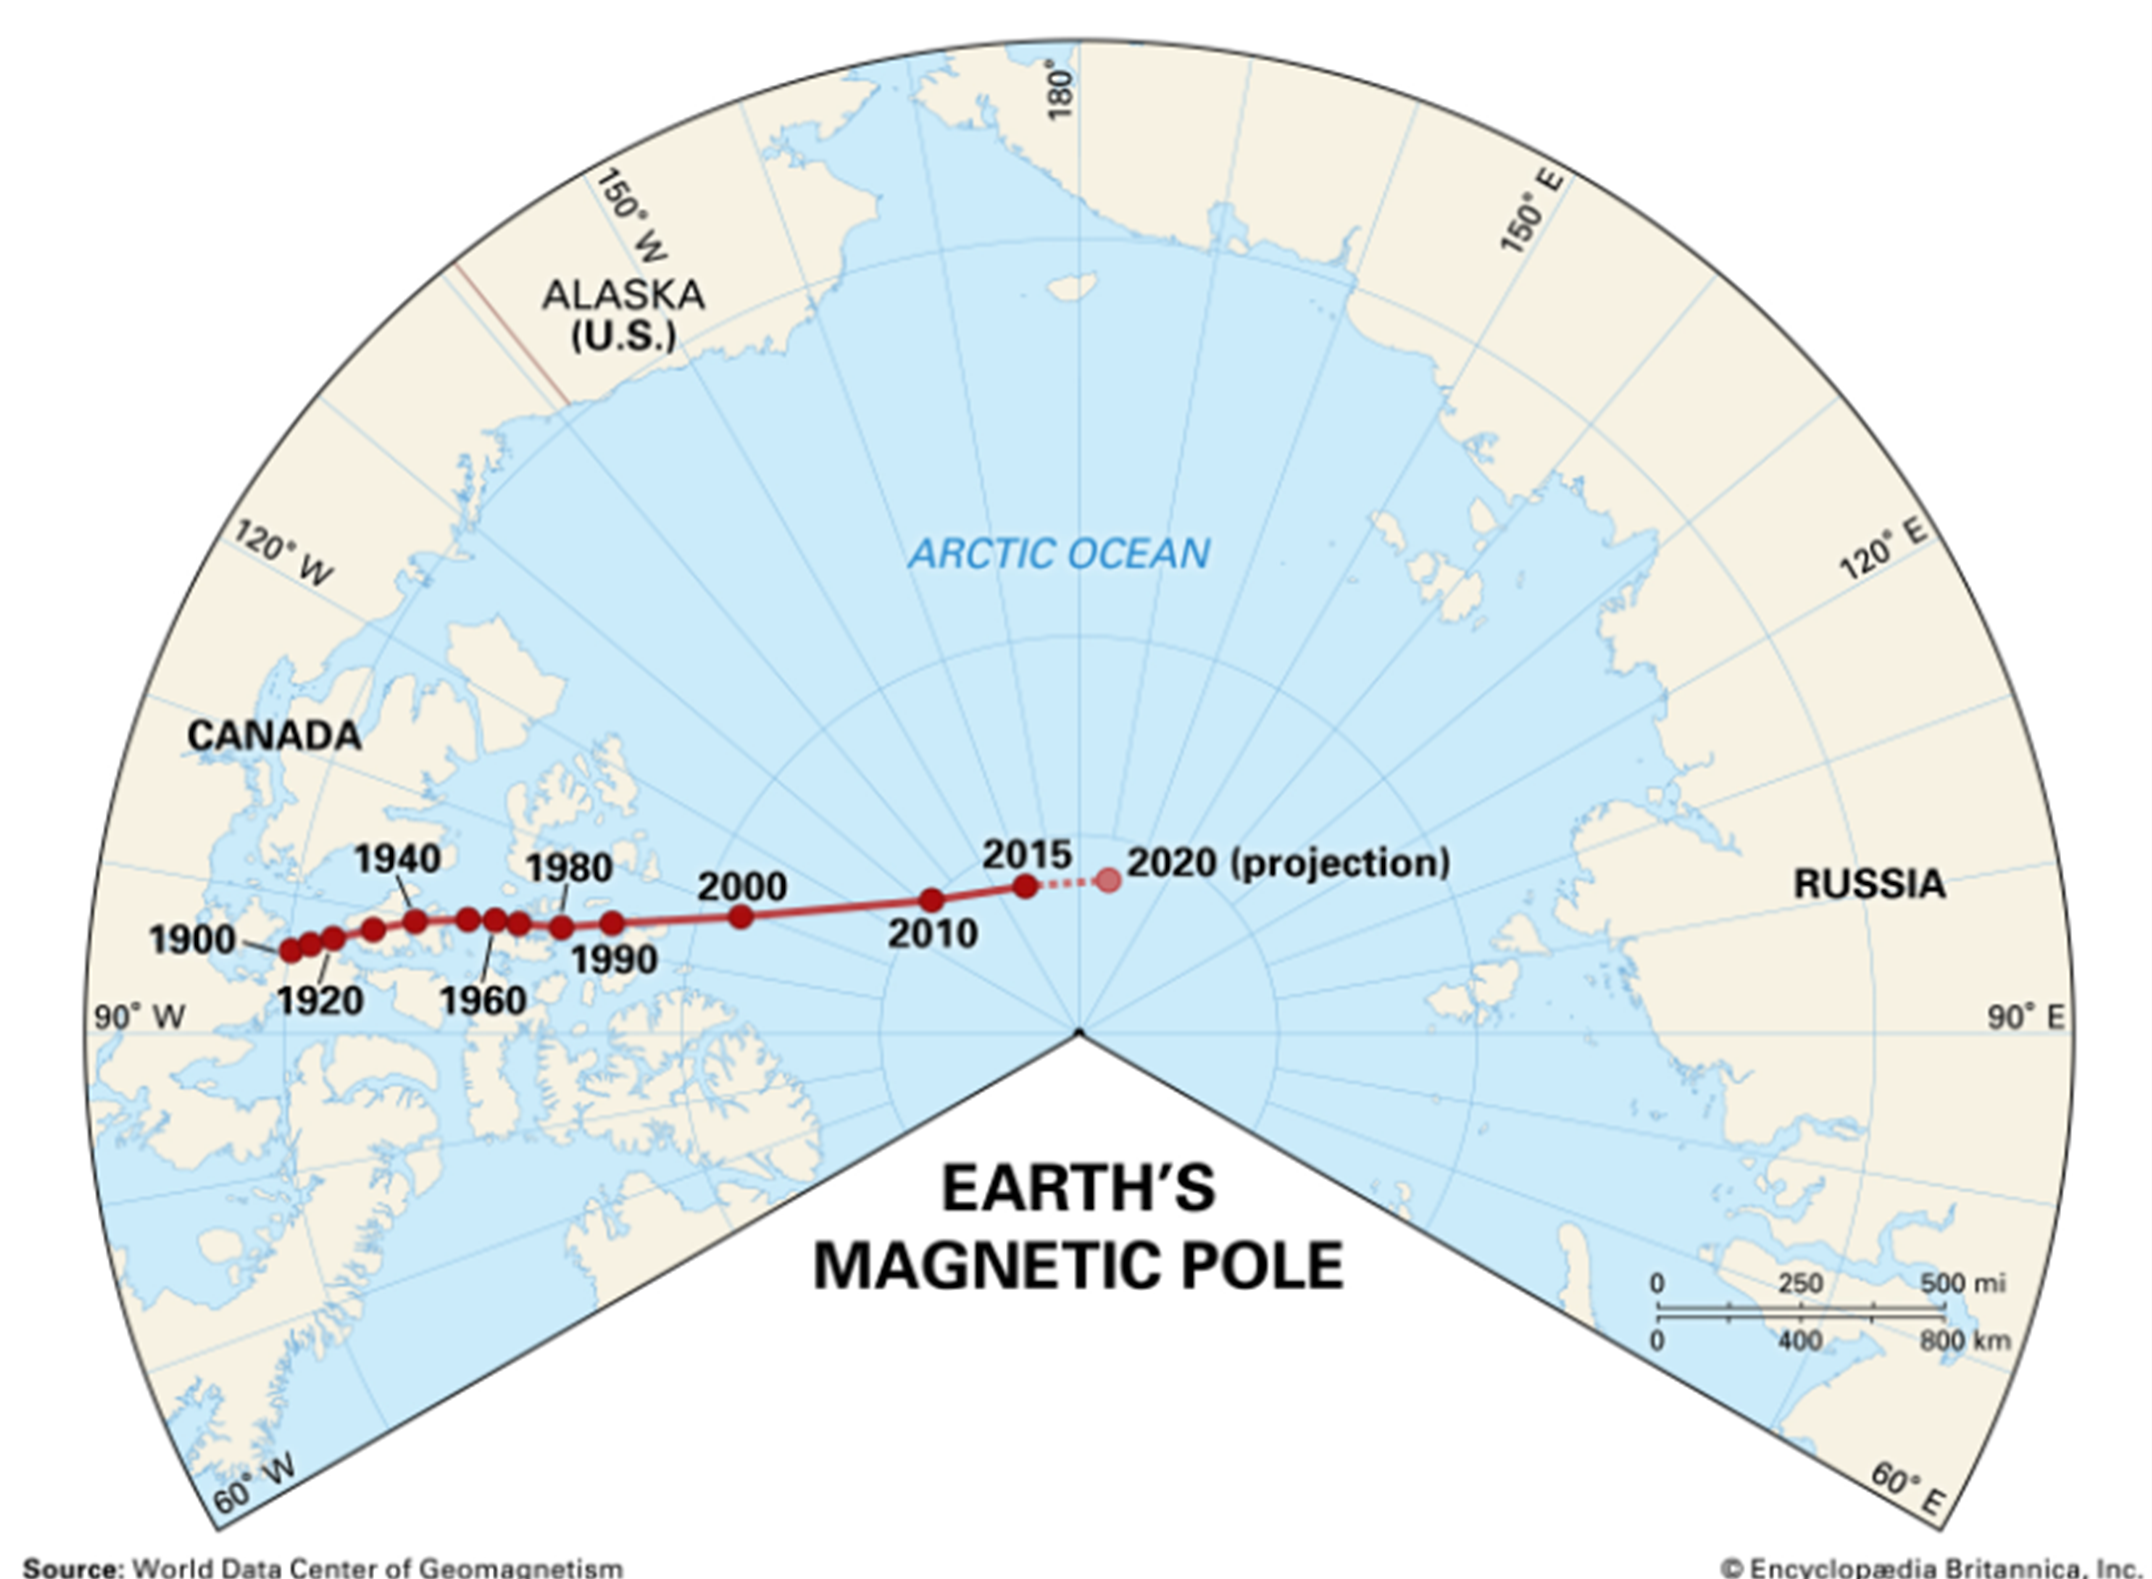
\includegraphics[width=0.5\columnwidth]{figures/magnetisk-nordpol}
\caption{Posisjonen til den magnetiske Nordpolen de siste 100 årene. \parencite{IncEncyclopediaBritannica}}
\label{fig:magnetisk-nordpol}
\end{figure}

Det er viktig å forstå forskjellen mellom magnetisk nord og faktisk nord ved orientering basert på jordens magnetiske felt. 
Jordens magnetiske felt varierer fra plass til plass og derfor er det avvik mellom faktisk nord og magnetisk nord. 
Den magnetiske Nordpolen er ikke et fast punkt som den faktiske Nordpolen. Den magnetiske Nordpolen flytter på seg over tid, 
og avhenger blant annet av hvordan jordens masse forflytter seg. Dette vil si at magma under de tektoniske platene og 
vann/is vil påvirke hvordan den magnetiske polen forflytter seg . Figur \ref{fig:magnetisk-nordpol} viser hvordan 
den magnetiske Nordpolen har forflyttet seg det siste århundret. 
I tillegg til avvik mellom polene og magnetfeltet er det også lokale variasjoner som gjør at kompass kan vise feil. 
Dette kan komme av lokale ansamlinger av metaller i jordskorpen eller bygninger i urbane miljøer. 
I 2007 utførte NGU en aeromagnetisk undersøkelse over Tromsø for å kartlegge variasjoner i de lokale magnetfeltet. 
Resultatet av denne undersøkelsen vises i figur \ref{fig:magnetisk-nordpol}. Undersøkelsen viser at blant annet områder på Kvaløya og 
Senja har økt magnetfelt i forhold til andre plasser. Derfor er det tenkelig at kompassmisvisningen vil være større i disse områdene. 
\parencite{Kartverket} 

\begin{figure}[htp]
\centering
\includegraphics[width=0.5\columnwidth]{figures/aeromagnetisk-kart}
\caption{Aeromagnetisk anomalikart fra undersøkelsen utført av NGU i 2007. \parencite{Gellein2007}}
\label{fig:aeromagnetisk-kart}
\end{figure}

\subsection{Akselerometer}
Et akselerometer er en sensor som måler akselerasjon i en, to eller tre retninger. 
Akselerometeret benyttes ofte sammen med et gyroskop for orientering og styring av fly, droner, 
raketter og ubåter. I tillegg brukes de til skjermorientering i smarttelefoner, 
vibrasjonsmåling i bygninger og kollisjonssensorer i biler. \parencite{Balchen2000}
Prinsippet for alle akselerometer er at det er en fast del og en løs del som typisk henger i en fjær. 
Dette fører til at den løse delen vil ha en treghet i forhold til den faste delen som 
vil bevege seg med det sensoren er festet til. \parencite{Balchen2000}

\subsubsection{MEMS-akselerometer}
Mikroelektromekaniske systemer er en samlebetegnelse på små systemer som utnytter både elektroniske og 
mekaniske prinsipper for å utføre en oppgave. Det er akselerometer bygget på denne teknologien som er 
mest vanlig i forbrukerelektronikk, blant annet fordi de kan lages så små. MEMS-akselerometer består av 
en masse som beveger seg langs en akse. Denne massen har små pinner som stikker ut til siden. 
Disse går imellom tilsvarende pinner som er statiske. Når det oppstår en akselerasjon langs aksen som 
sensoren måler vil avstanden mellom disse pinnene forandre seg. Når dette skjer vil det oppstå en endring 
i kapasitansen mellom de faste pinnene og de som forflytter seg. 
Det er denne endringen i kapasitans som benyttes for å beregne akselerasjonen. 

\begin{figure}[htp]
    \centering
    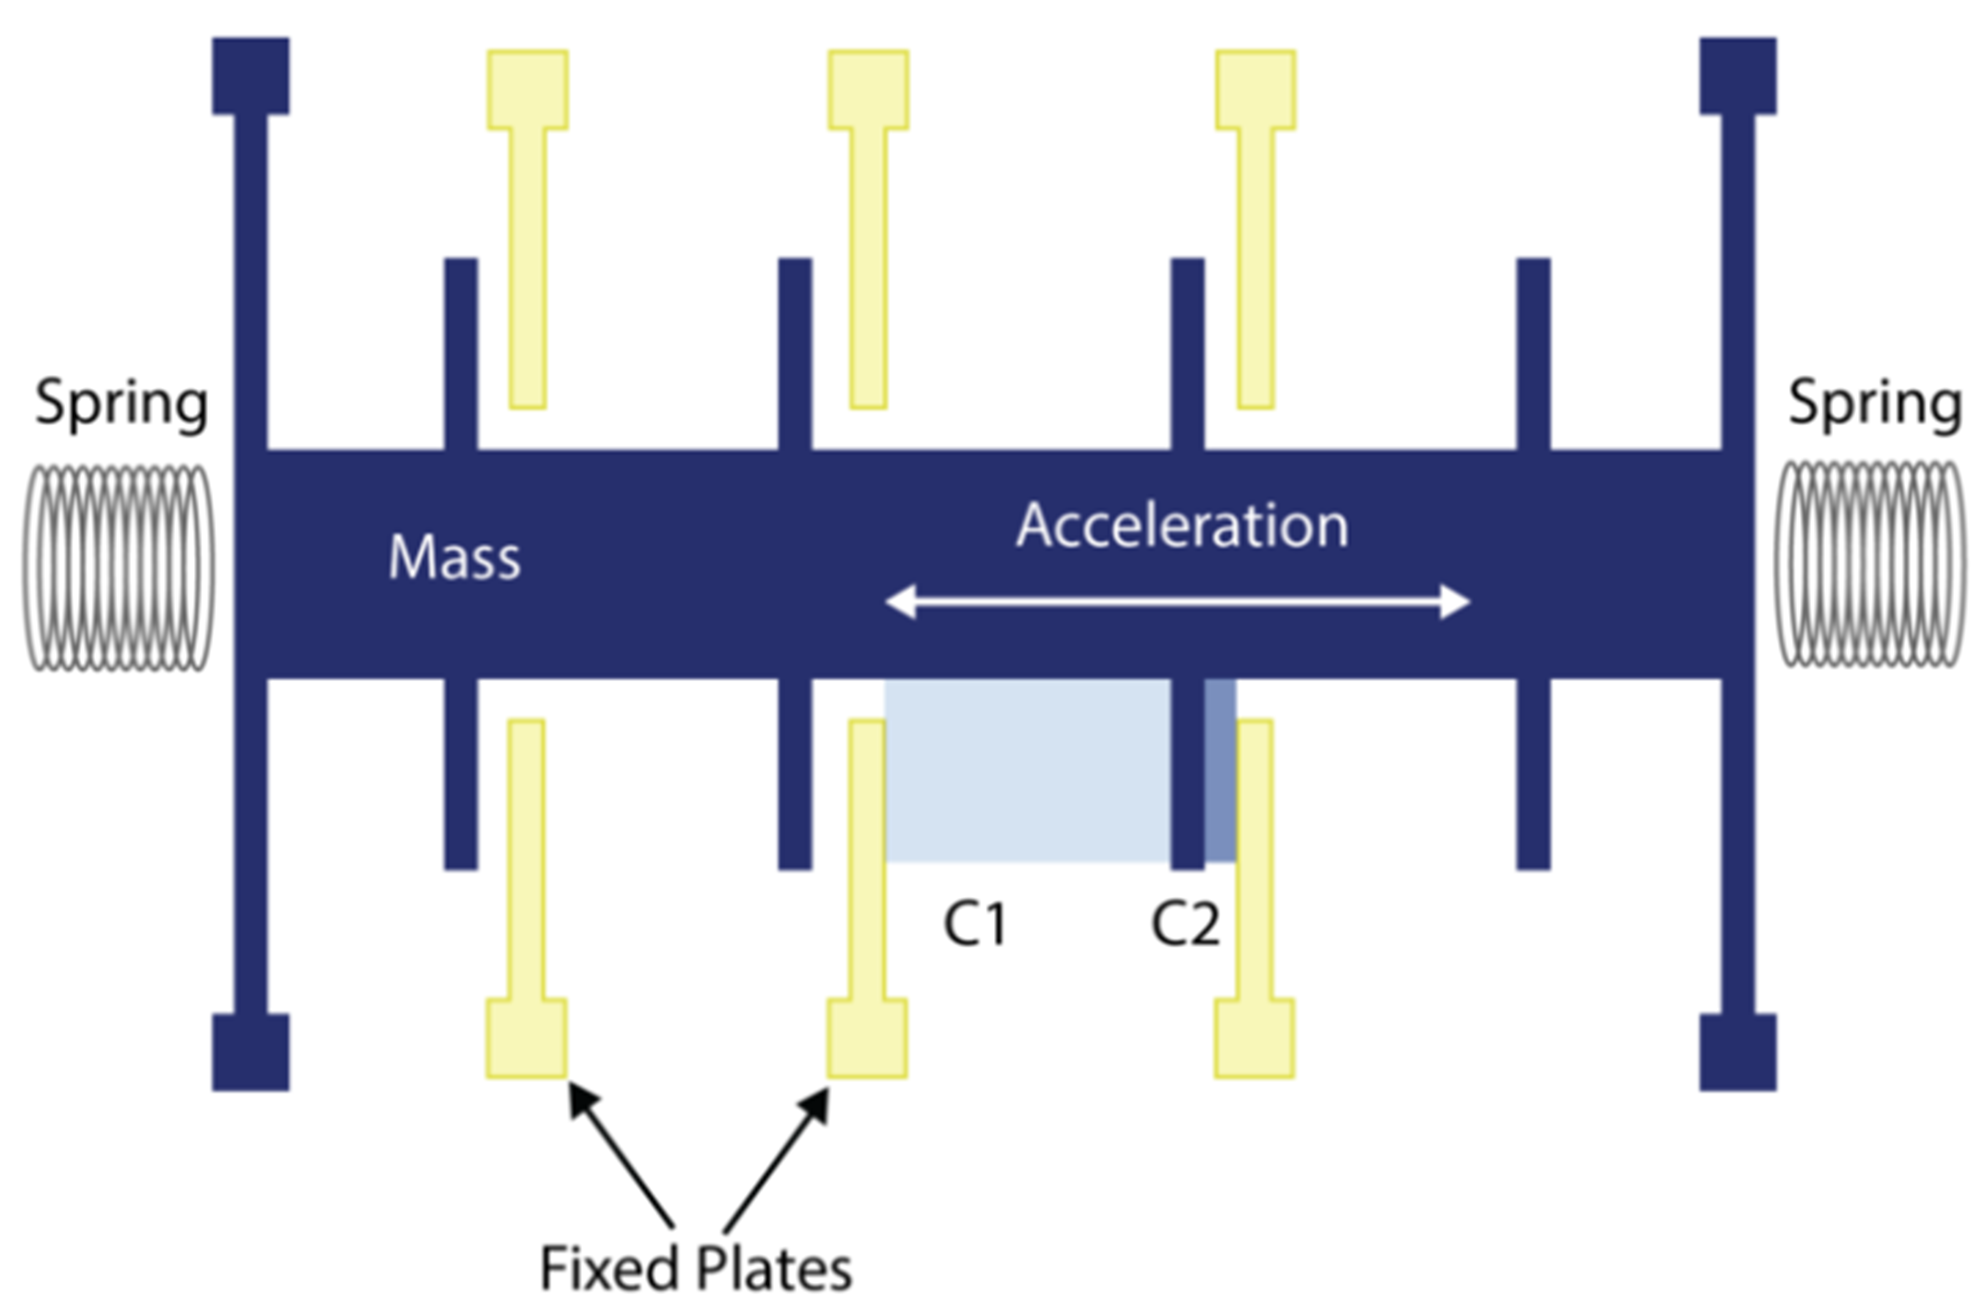
\includegraphics[width=0.5\columnwidth]{figures/mems-aks}
    \caption{MEMS-akselerometer. \parencite{LevelDevelopments2020}}
    \label{fig:mems-aks}
\end{figure}

\subsubsection{Piezoelektrisk akselerometer}
Den piezoelekstriske effekten kan også brukes til å beregne akselerasjon. 
Effekten går ut på at enkelte krystaller skaper en spenning ved deformering. \parencite{Gron2021piezo}
Ved å koble til elektroder på hver side av et krystall kan kraften av en masse som presser mot 
krystallen beregnes ut ifra spenningen som oppstår over krystallen. Ut ifra kraften og massens 
vekt kan akselerasjonen beregnes. Prinsippet for dette akselerometer er beskrevet ifigur \ref{fig:piezo-aks}. 
Basen vil være koblet statisk uelastisk til en gjenstand. Og når denne gjenstanden beveger seg i retningen som 
pilen viser vil en kunne beregne akselerasjonen ved hjelp av elektrodene på hver side av krystallen. 

\begin{figure}[htp]
\centering
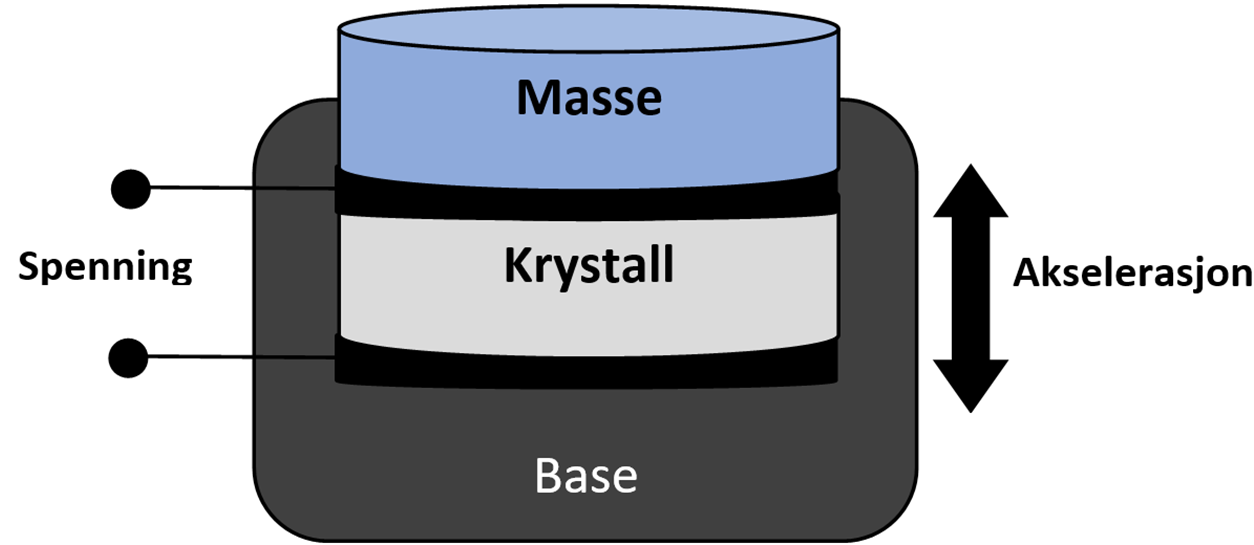
\includegraphics[width=0.5\columnwidth]{figures/piezo-aks}
\caption{Piezoelektrisk akselerometer.}
\label{fig:piezo-aks}
\end{figure}

\subsection{gyroskop}
Et gyroskop, eller en gyrosensor måler endring i rotasjon langs pitch, roll og yaw aksene. 
I likhet med akselerometer og magnetometer er gyroskop som benyttes i elektronikk bygget på MEMS-teknologi. 
MEMS-gyroskop benytter coriolisakselerasjonen som er en akselerasjon som oppstår på et legeme som 
beveger seg i en rett linje på et roterende referansesystem. Coriolisakselerasjonen vil da oppstå vinkelrett på bevegelsen. \parencite{Gron2021coriolis}
Figur \ref{fig:mems-gyro} viser et eksempel på et MEMS-gyroskop. Det består av en vibrerende struktur som holder en deteksjonsstruktur (grønn). 
Når sensoren er stabil, vil deteksjonsstrukturen bevege seg frem og tilbake med den vibrerende strukturen. 
Ved rotasjon vil deteksjonsstrukturen skyves ut til siden på grunn av coriolisakselerasjonen. 
For å beregne rotasjonen benyttes endringen i kapasitansen mellom kammene i deteksjonsstrukturen som oppstår ved forskyvningen. 

\begin{figure}[htp]
    \centering
    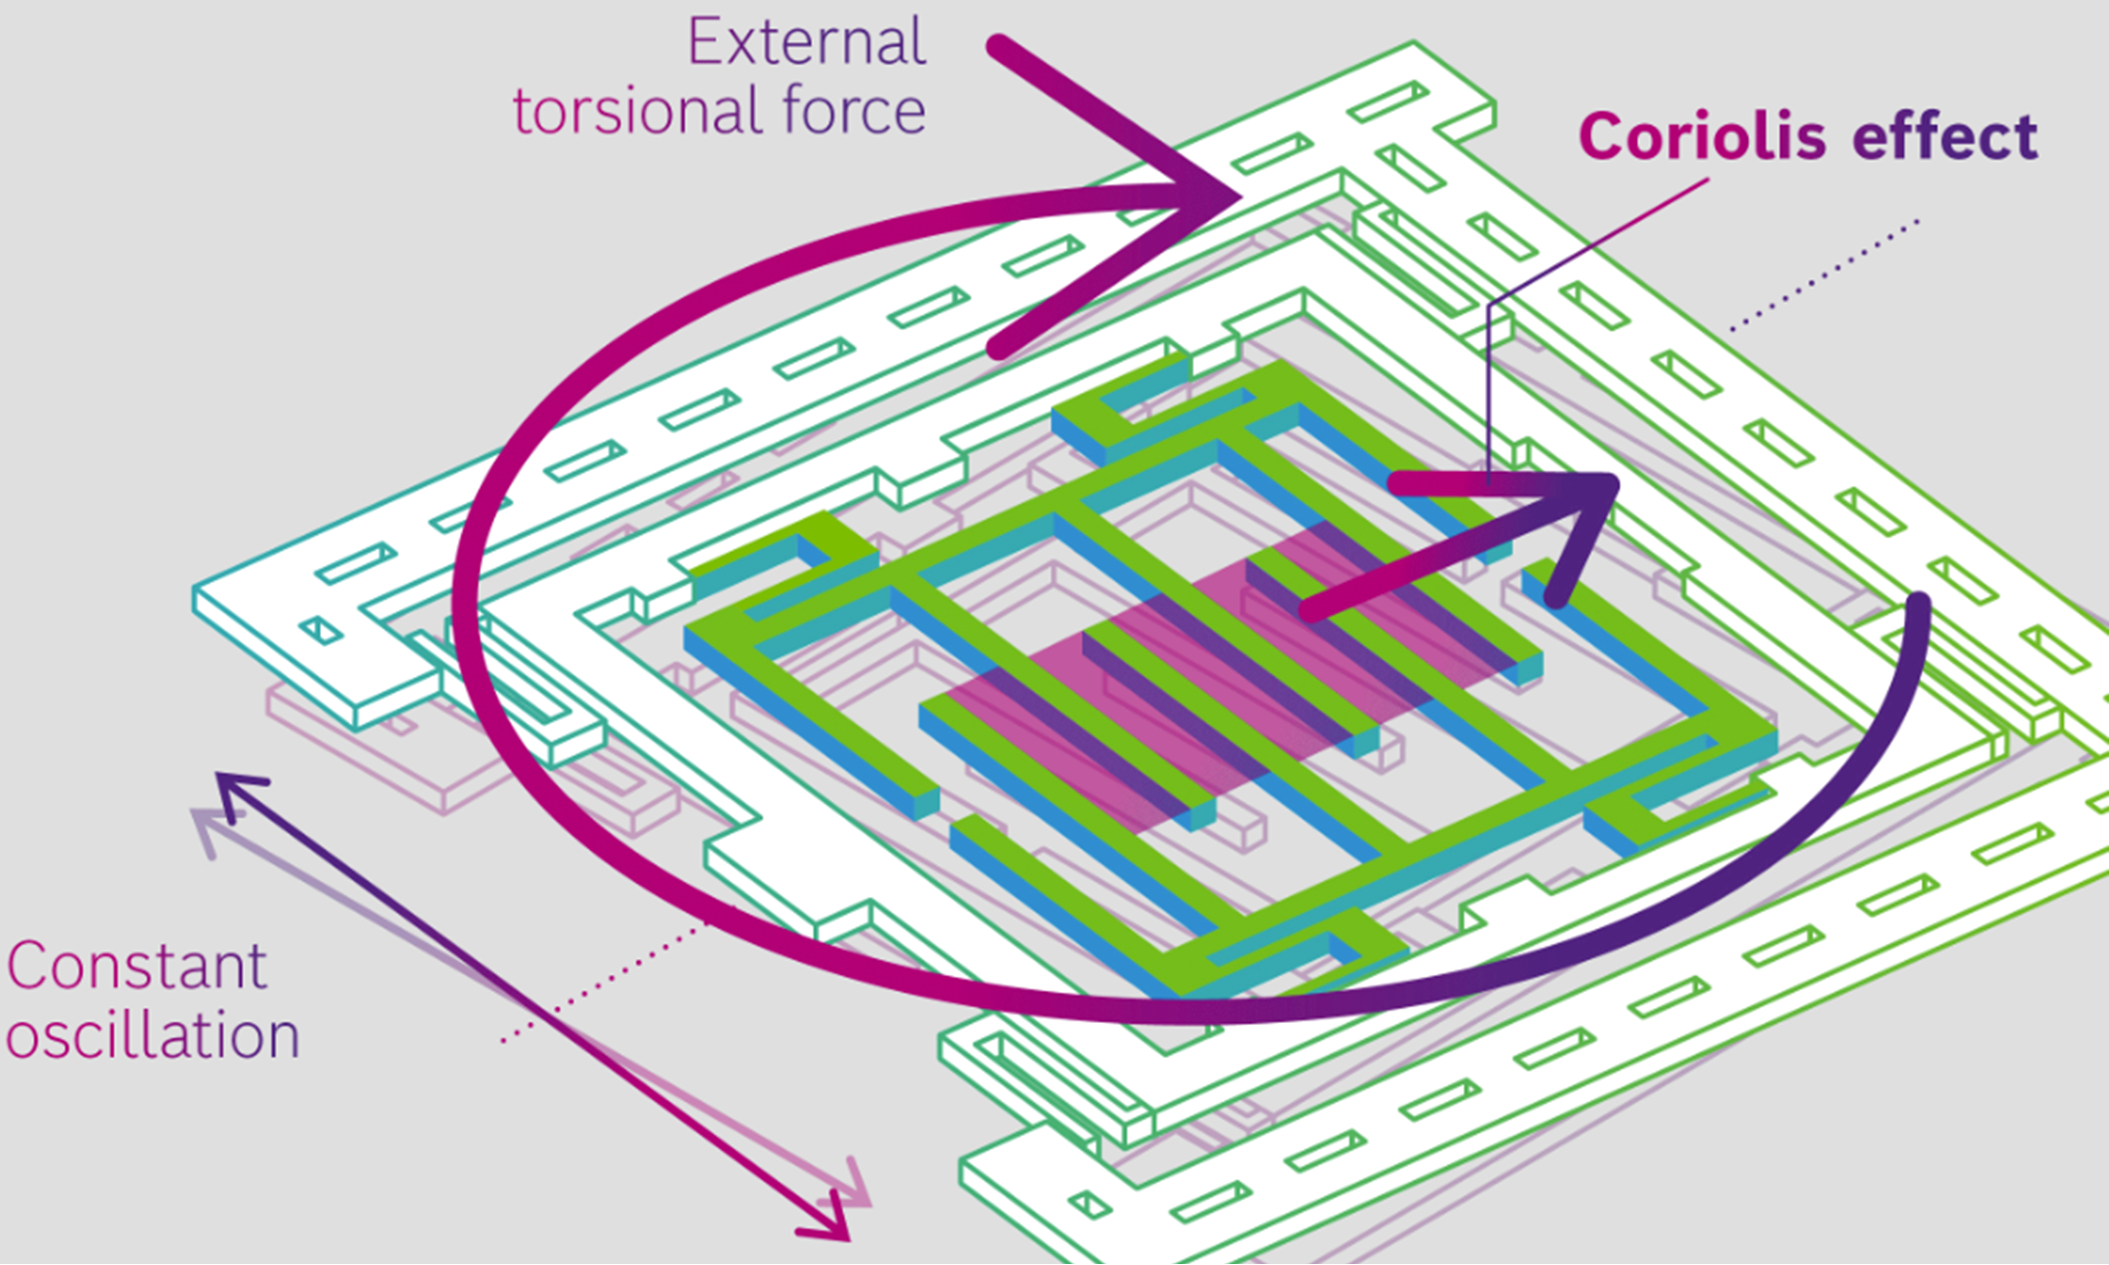
\includegraphics[width=0.5\columnwidth]{figures/mems-gyro}
    \caption{MEMS-gyroskop. \parencite{Bosch}}
    \label{fig:mems-gyro}
\end{figure}

Figur \ref{fig:mems-gyro} viser en enkel rotasjonssensor som kun vil detektere rotasjon rundt 
aksen som står vinkelrett på deteksjonsstrukturen. For å detektere rotasjon i tre akser må 
flere slike rotasjonssensorer med forskjellig orientering kombineres. \parencite{Bosch}


\subsection{Barometer}
Barometer er ett instrument eller en elektrisk sensor som måler lufttrykk. 
Prosjektet tar for seg barometer for å beregne høyde, i prosjektet blir 
elektrisk sensor som sensoren i figur \ref{fig:bme280} brukt. Luftrykket på 
jorda minker ved økning i høyde, denne endringen i luftrykket kan bli brukt for å estimere høyde. 
Luftrykket kan endret av lokale trykkvariasjoner på jorda. Her har vær, klima, 
tidevann og temperatur noe å si. Ved bruk av barometer for høyde 
beregninger er det derfor nødvendig å kalibrere barometeret først. Bruk av barometer for høydeangivelse 
innendørs kan gi problemer med uønskede trykkendringer. Her kan åpning av dører eller 
bruk av ventilasjonssystemer skape store trykkforskjeller.
\parencite{Gron2021piezo}

\begin{figure}[htp]
    \centering
    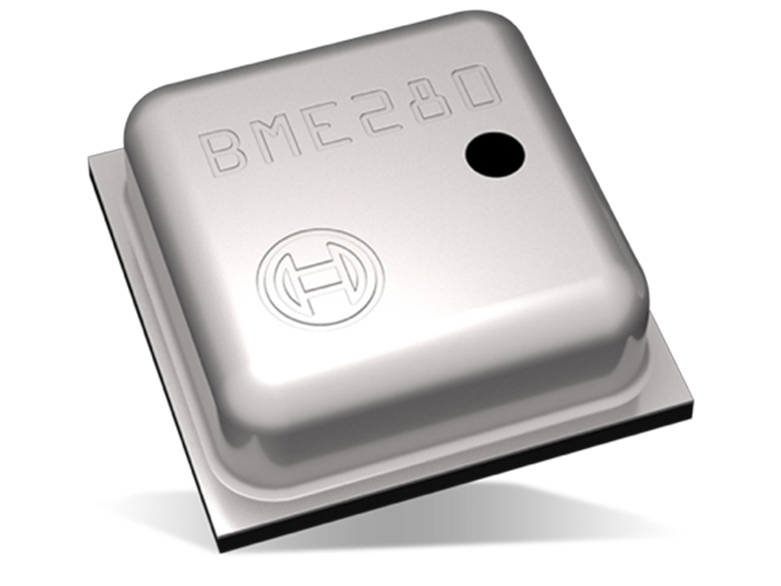
\includegraphics[width=0.5\columnwidth]{figures/bme280}
    \caption{BME280. \parencite{Bosch}}
    \label{fig:bme280}
\end{figure}

\subsection{PID-regulator og posisjon hold}
PID- regulatoren er en reguleringssløyfe som består av proporsjonalt, integrasjon og derivasjons-ledd. 
Reguleringssløyfen arbeider for å minke forskjellen mellom målt verdi og ønsket verdi.

\begin{figure}[htp]
    \centering
    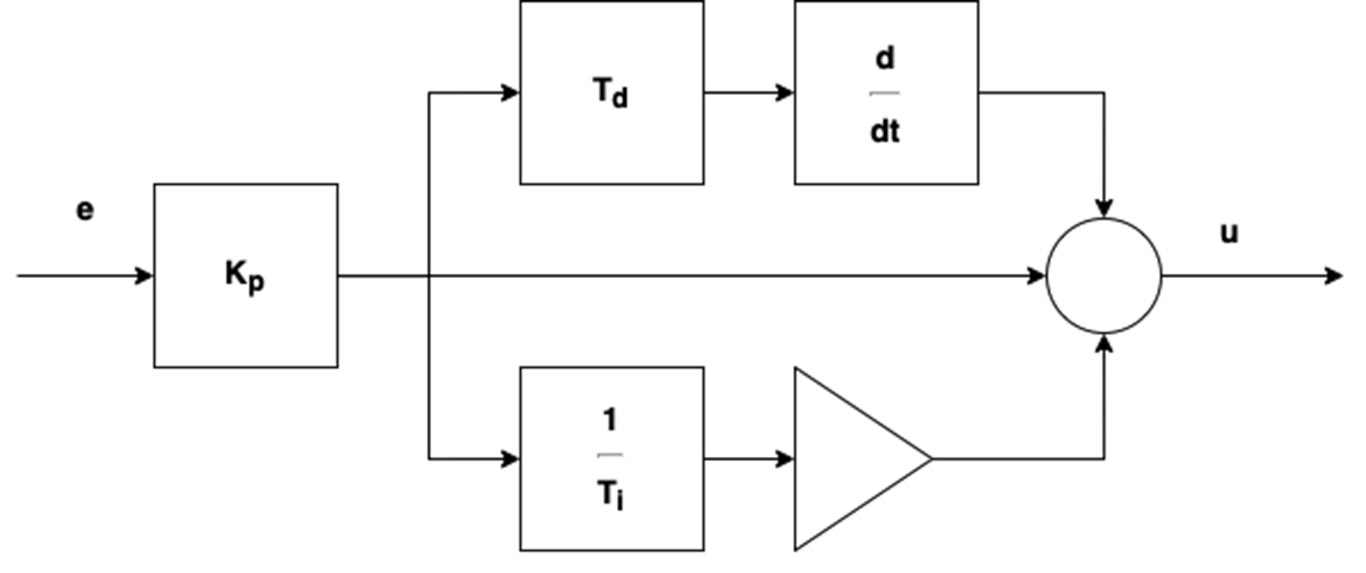
\includegraphics[width=0.7\columnwidth]{figures/reguleringssloyfe}
    \caption{PID-reguleringssløyfe.}
    \label{fig:reguleringssloyfe}
\end{figure}

\begin{itemize}
\item P: Proposjonalt ledd. $K_pe(t)$
\item I: Integrat ledd. $K_i \int_0^t e(t) dt$
\item D: Derivat ledd. $ K_d \frac{d e(t)}{dt} $
\end{itemize}

D-leddet gir pådrag gitt av akselerasjon.  D-leddet øker båndbredden til regulatoren slik hurtig regulering er mulig. 
Ved høye frekvenser kan d-leddet gi uønsket støy. Filtrering er ofte nødvendig for å fjerne støyen. \parencite{Balchen2000} 

\subsubsection{PID-regulering for droner}
For droner brukes PID regulatoren for å regulere rotasjon og posisjon til dronen. 
For å holde rotasjonen til dronen stabilt blir hver akse sin regulator justert for å minimere avvik. 
Dette kan være utfordrende å gjøre, analyse av logger og visuell inspeksjon av flyvninger kan hjelpe for å justere regulatorene.

Det er mulig å sette PID-regulator for å la dronen selv stabilisere seg. 
Her vil PID-regulatoren regulere hvor raskt og aggressiv dronen er for å rette opp rotasjonen. 
Mange droner har muligheten å sette dronen i Posisjon-hold modus. 
Denne funksjonen trenger PID-regulering for å bestemme hvor raskt og aggressivt dronen skal jobbe for å holde posisjonen. 

Transferfunksjon: 9.48
\[h_r(s) = K_p(1+\frac{1}{T_is}+T_ds) = K_p \frac{1+T_i(s)+T_iT_ds^2}{T_is} \approx K_p \frac{(1+T_is)(1+T_ds)}{T_is}\]

Filtrering
Støy. Statisk filter Dynamisk filter.


\subsection{Extended kalman filter (EKF)}
Kalman Filter er en algoritme som kan predikterer neste status på ett system ved å bruke observert data fra 
sensorer og tidligere status til systemet. For system med u-lineære bevegelser slik som droner og roboter har, 
blir Extended Kalman Filter brukt for å finne posisjon, rotasjon, hastighet og akselerasjon til systemet. 
Bruk av EKF vil kunne gi bedre estimat på status av ett system enn hva en enkel sensor kan. Dette fungerer ved at 
EKF kan bedre filtrere bort støy og avvik på en sensorer ved sammenligning av andre sensorer. 
Målinger fra sensorer slik som IMU-er kan være utsatt for mye støy, det kan EKF hjelpe å filtrere bort, 
eller avvise data ved for stort avvik. 

\begin{figure}[htp]
    \centering
    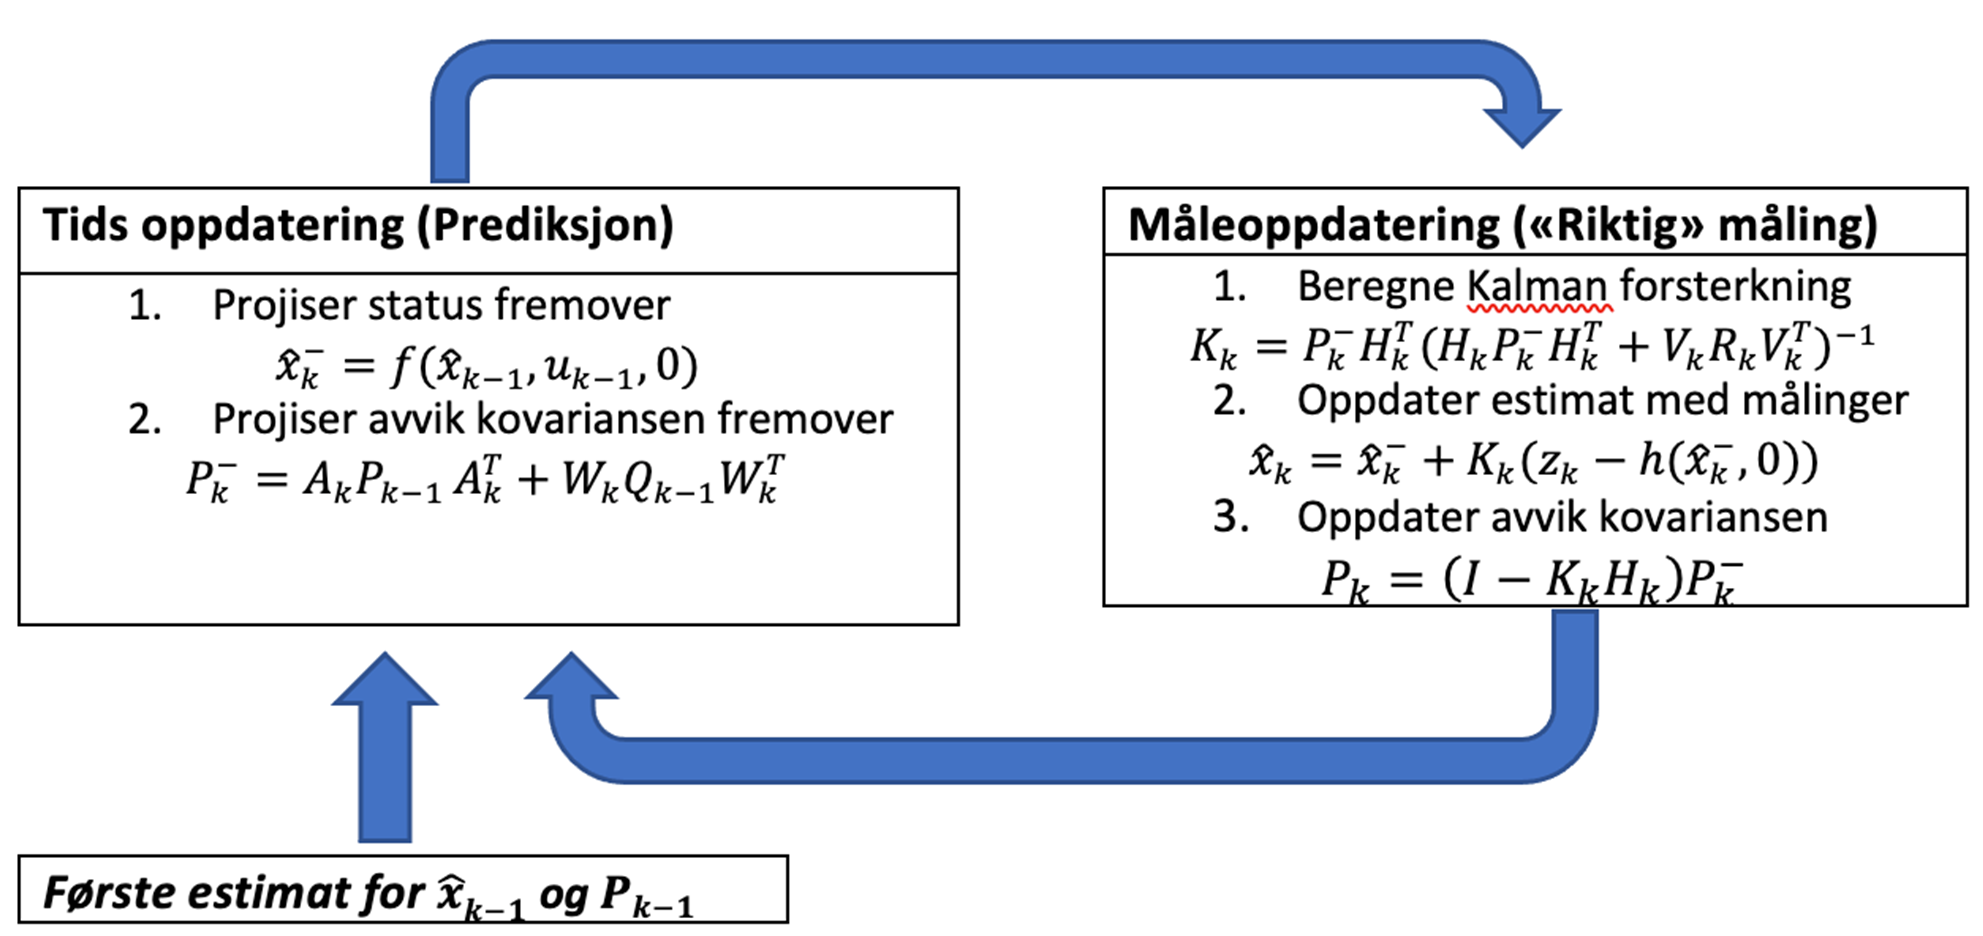
\includegraphics[width=1\columnwidth]{figures/ekf}
    \caption{EKF algoritme.}
    \label{fig:ekf}
\end{figure}

Figur \ref{fig:ekf} viser hvordan EKF oppdateres. EKF prediktere neste status på systemet fra forrige estimat og 
deretter korrigere dette estimatet med målinger i nåtid fra sensorer. For en drone vil sensorer fra IMU og kompass 
gi rotasjon og akselerasjon. GNSS eller andre posisjonssystem og barometer vil kunne gi posisjonen og høyden til dronen. 
EKF samler dataen fra sensorene og gir estimat på posisjon, og rotasjon, fart og akselerasjon. 
Dette estimatet kan vider bli brukt til å regulere dronen sitt pådrag for å styre dronen, 
dette kommer rapporten mer inn på i PID-regulering avsnittet. \parencite{ArdupilotDevTeam}


\subsection{Multirotor}
Multirotor er en samlebetegnelse på alle typer droner med 3 eller flere motorer. Den vanligste typen er quadcopter, altså en drone med fire armer og en motor på hver arm. Figur \ref{fig:dji-air-2} viser et populært quadcopter fra DJI.

\begin{figure}[htp]
    \centering
    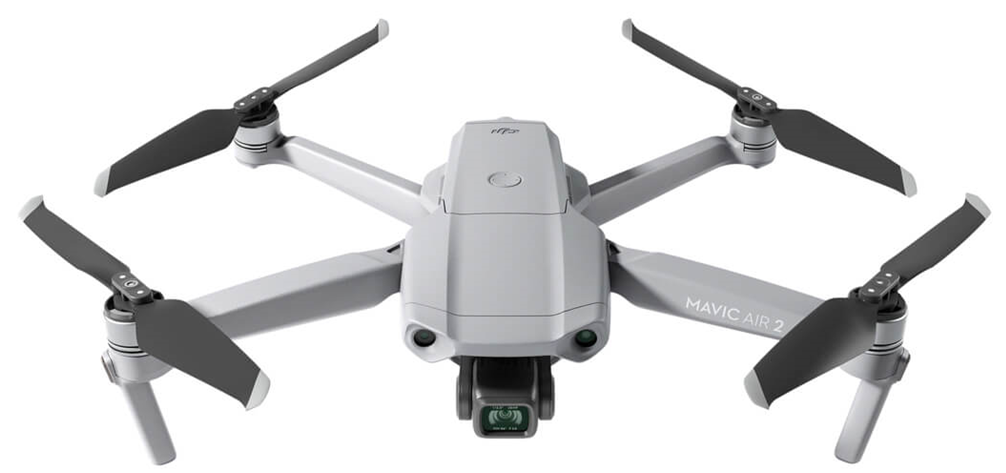
\includegraphics[width=0.7\columnwidth]{figures/dji-air-2}
    \caption{DJI Air 2}
    \label{fig:dji-air-2}
\end{figure}

\subsubsection{Komponenter}
Et quadcopter består i sin enkleste grad av en ramme, fire motorer, fire propeller, en flight controller, en mottaker og fire ESC ’er.
Flightcontrolleren er hjernen i drona. Denne består av en liten datamaskin, IMU og porter. Oppgaven til flightcontrolleren er å ta imot signaler fra sensorer og radiokontroller, og gi signal videre til ESC for å styre hastigheten til de individuelle motorene. 

\begin{figure}[htp]
    \centering
    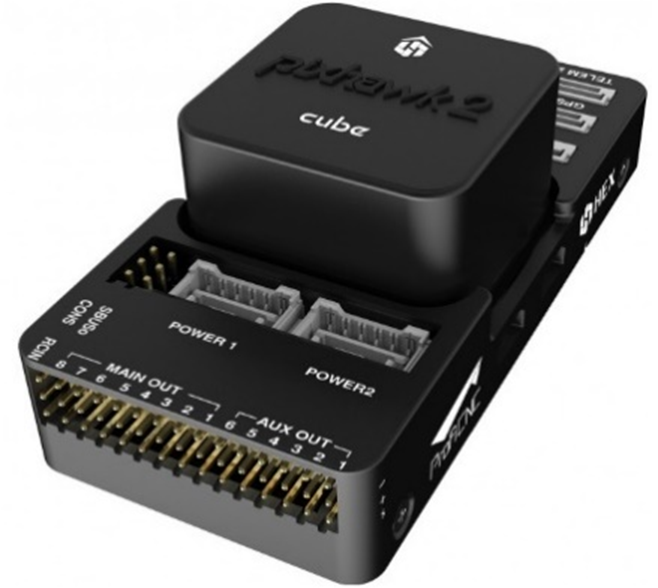
\includegraphics[width=0.4\columnwidth]{figures/pixhawk}
    \caption{Pixhawk Cube}
    \label{fig:pixhawk}
\end{figure}

Pixhawk, som vist i figur \ref{fig:pixhawk}, er en populær flightcontroller til utvikling av droner. Denne kan kjøre ardupilot programvare, som er opensource programvare laget for ROV, fly og multirotor. Grunnen til at pixhawk og ardupilot er så mye brukt er at det enkelt kan kobles på sensorer og utstyr, og man kan enkelt gjøre egne endringer i programvaren. 
En mottaker kobles til flightcontrolleren for at man skulle kunne gjennomføre manuell flygning og kunne bytte mellom ulike moduser under automatisk flyging med en radio. 
ESC (Electronic Speed Controller) er fartskontrolleren til motoren. Denne får signal fra flightcontrolleren om hvor fort motorene skal spinne, og gir deretter tilsvarende strøm til motorene. 

\begin{figure}[htp]
    \centering
    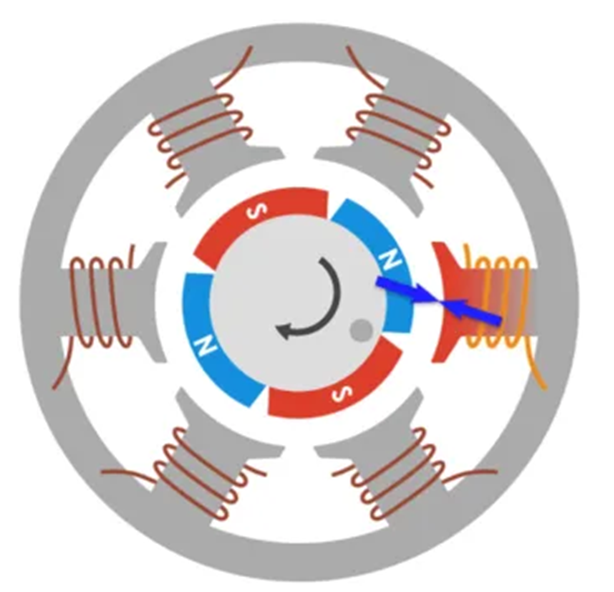
\includegraphics[width=0.4\columnwidth]{figures/dc-motor}
    \caption{Børsteløs DC-motor}
    \label{fig:dc-motor}
\end{figure}

Børsteløse DC motorer blir oftest brukt på quadcopter. Disse består av to deler. En stator og en rotor. Statoren er bygget opp av flere viklinger med kobbertråd. Rotoren er laget av en magnet. Når det blir satt strøm på ulike kobbertråd viklinger vil det skape et magnetfelt som får magneten i rotoren til å spinne i ønsket retning, som vist i Figur 21. På denne måten kan man enkelt øke og minke hastigheten på motoren.

\subsubsection{Styring}
En multirotor styres som tradisjonelle fly med pitch, yaw og roll. Illustrert i figur \ref{fig:akser}

\begin{figure}[htp]
    \centering
    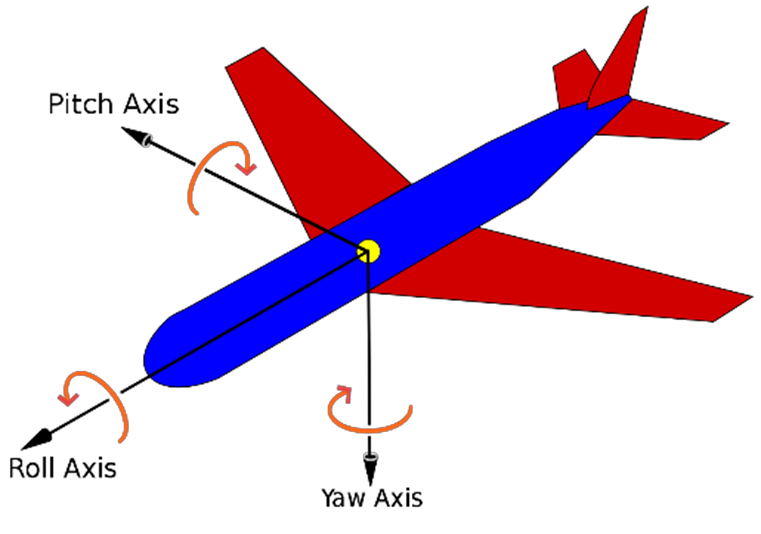
\includegraphics[width=0.4\columnwidth]{figures/akser}
    \caption{Akser på et luftfartøy}
    \label{fig:akser}
\end{figure}

For å rotere i de ulike aksene, må motorene spinne i ulike hastigheter.Figur \ref{fig:motor-rotasjon} viser det vanligste oppsettet for motorenes rotasjon:

\begin{itemize}
\item Pitch: for å få dronen til å bevege seg fremover må motor 3 og 4 spinne raskere enn motor 1 og 2.
\item Roll: For å få dronen til å bevege seg til venstre må motor 2 og 3 spinne raskere.
\item Yaw: For å dreie dronen mot høyre må motor 2 og 4 spinne fortere.
\end{itemize}

\begin{figure}[htp]
    \centering
    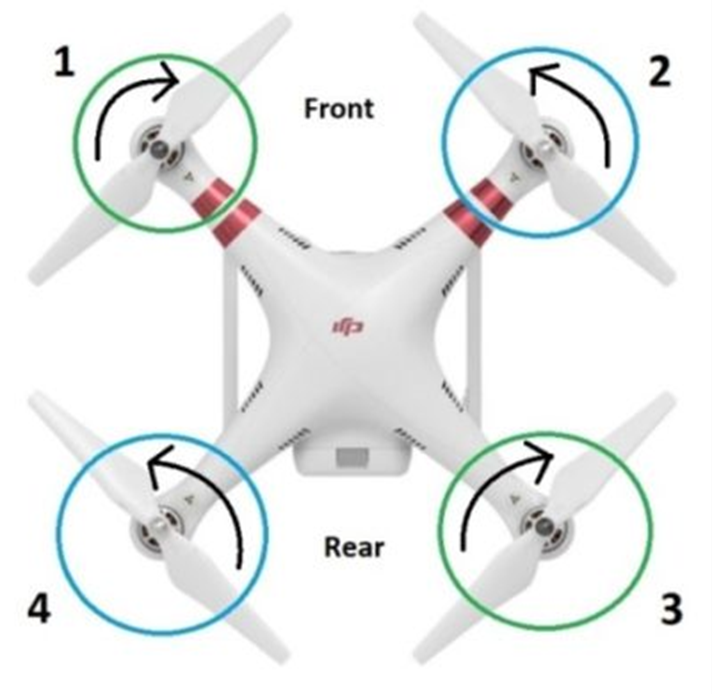
\includegraphics[width=0.4\columnwidth]{figures/motor-rotasjon}
    \caption{Rotasjonsretning på multirotor}
    \label{fig:motor-rotasjon}
\end{figure}

I tillegg til disse tre brukes throttle. Øking av throttle gjør at alle motorene spinner fortere, og dronen vil da få en akselerasjon normalt på planet til propellene. Altså rett opp dersom dronen står stille på bakken.
Dronen styres da ved å bruke pitch, roll og yaw for å oppnå ønsket rotasjon, og throttle for å skape en akselerasjon i ønsket retning. Illustrert i figur \ref{fig:krefter-pa-drone}. 

\begin{figure}[htp]
    \centering
    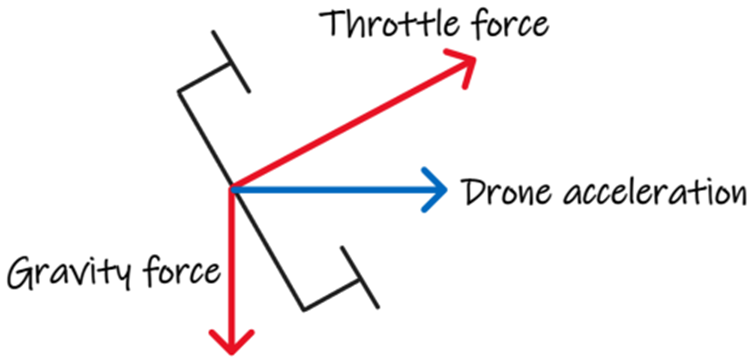
\includegraphics[width=0.5\columnwidth]{figures/krefter-pa-drone}
    \caption{Krefter i fartsretningen på en multirotor}
    \label{fig:krefter-pa-drone}
\end{figure}


\newpage
\section{Sikkerhet og regelverk}
Dette kapittelet tar for seg sikkerhetstiltakene og reglene som gruppen har fulgt. Målene for gruppen var å: Ikke skade personer eller omgivelsene med dronen. Ikke ødelegge kritiske komponenter. Ikke interferere andre sendinger i nærheten, f.eks flytrafikk og radiosamband.

\subsection{Sikkerhetstiltak for operasjonene}
Det ble utført flere tiltak for å få dronen trygg for innendørs bruk. Gruppen vurderte at flyvninger med udekket propeller kunne få for store konsekvenser.  Det ble derfor designet propellerbeskyttere til dronen.
Gruppen har bare 2 UWB-tags tilgjengelig, og disse må ikke bli ødelagt. For å unngå å skade disse ble det designet ett “rullebur” for å forhindre skade under krasj eller harde landinger. 
De 3d-printet delene ble designet for å deformere seg eller knekke for å minke nedslag til dronen sine kritiske komponenter. Dette ble valgt siden 3d-printet deler er enkelt og billig å bytte ut. 

\subsection{Tiltak for drone på avveie}
For å alltid ha kontroll over dronen ble det brukt enn manuell-pilot under flyvningene. Den manuell-piloten sin oppgave var å ta over kontroll om drone kom på avveie på grunn av programfeil osv.  Det ble også brukt basestasjon for å kontrollere og overvåke dronen. Personell på basestasjon overvåkte kritiske verdier som batteribruk og helsen til sensorene. 
Ved tap av manuell-kontroll link ble dronen programmert til å kutte motorene, dette ble valgt siden dronen kan uføre større skade med å prøve å lande ta seg selv 
For å unngå brukerfeil under flyvning ble sjekklister implementert. 

\subsection{Regelverk for droneflyvning}
For innendørsflyvning gjelder ikke regelverket for droner. Slik at her kunne en flyve uten operasjonslisens. 
For utendørsflyvning har en av gruppens deltaker registrert seg i åpen kategori og har kommersiell forsikring. 

\subsection{Regelverk for sendinger}
For sendingen i prosjektet er det ingen krav for tillatelser for bruk, men det er regler for hvilke frekvenser som kan brukes, hvilken sendestyrke som er lovlig og hvordan data blir sendt.
\begin{itemize}
\item Regelverket for kommunikasjon til dronen gjelder under forskrift om generelle tilatelser til bruk av frekvener (fribruksfirskriften), kap 3.8 Diverse utstyr for kortdistansekommunikasjon. https://lovdata.no/forskrift/2012-01-19-77/§33.8   
\item For regelverket for UWB posisjon blir regelverket for generelle tilatelser til bruk av frekvener (fribruksfirskriften), kap 35a følgt.   https://lovdata.no/forskrift/2012-01-19-77/§35a 
\end{itemize}

\section{Gjennomføring}

\subsection{Oppsett av UWB-tags og ankere}
Det første oppsettet av UWB-tags og ankere ble gjort på et grupperom. Ankerene ble plassert i henhold til Pozyx sin guide. 
Guiden sier at ankerene skal bli plassert:
\begin{itemize}
\item Høyt og i synsrekkevidde for taggen
\item Ikke i en rett linje, men rundt i rommet.
\item 2-20 meter fra hverandre
\item 20 cm vekk fra metall
\item Vertikalt, slik at antennen peker opp eller ned
\item I ulik høyde for å oppnå 3D posisjonering
\item I synsrekkevidde til hverandre dersom man ønsker å bruke auto kalibrering
\end{itemize}


(Pozyx, n.d.)
Ankerene ble plassert i vært hjørnet av rommet slik som figur \ref{fig:ankerplassering} viser. 
Det ene ankeret ble plassert høyere enn de andre for å oppnå 3D posisjonering.
Hjørnet nærmest det ene ankeret (ankeret til høyre på Figur 25) ble brukt som nullpunkt. 
Det ble brukt laser for å måle opp de andre ankrenes posisjon i forhold til dette punktet. 
Gulvet i rommet ble regnet som høyde 0. Ankerenes posisjoner i millimeter ble da:

\begin{center}
\begin{tabular}{||c c c c||} 
 \hline
 Anker ID & x-retning & y-retning & z-retning \\ [0.5ex] 
 \hline\hline
 0x0D7A & 27 & 44 & 1132 \\ 
 \hline
 0x6834 & 27 & 2787 & 2415 \\
 \hline
 0x684E & 4725 & 494 & 1165 \\
 \hline
 0x684F & 4725 & 2795 & 1184 \\ [1ex] 
 \hline
\end{tabular}
\end{center}

\begin{figure}[htp]
\centering
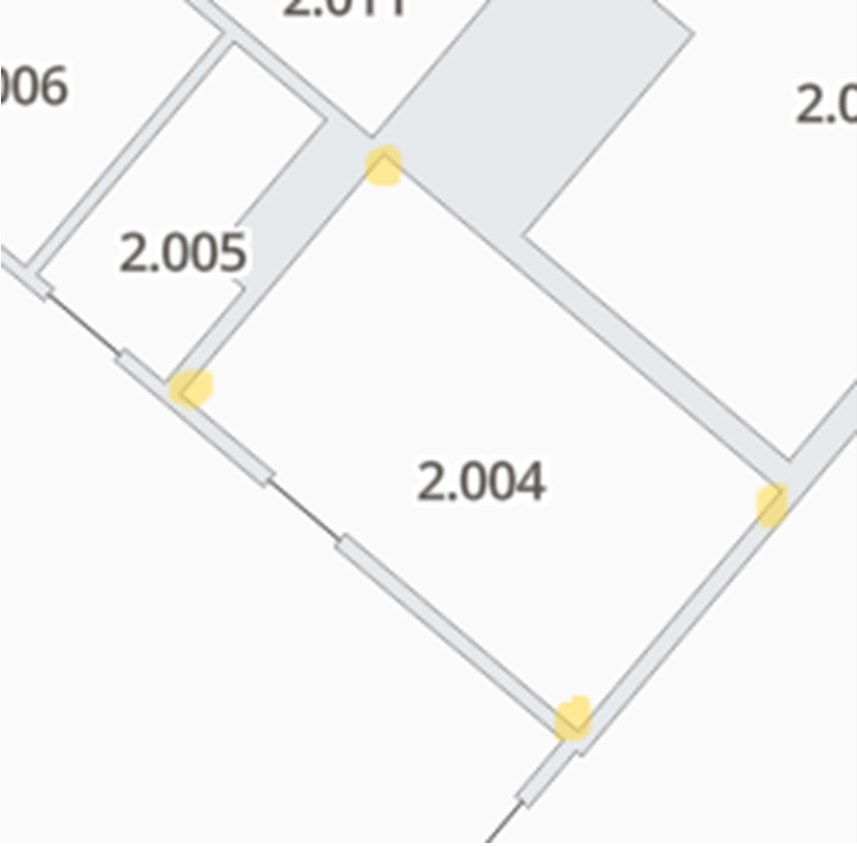
\includegraphics[width=0.5\columnwidth]{figures/ankerplassering}
\caption{Ankerplassering}
\label{fig:ankerplassering}
\end{figure}

Når ankrene var målt opp ble oppmålingen lagt inn i Pozyx Creator Controller, vist i figur \ref{fig:creator-controller}. 
Dette programmet ble brukt til å bekrefte at systemet fungerte, og at tagen greide å finne posisjonen sin.

\begin{figure}[htp]
\centering
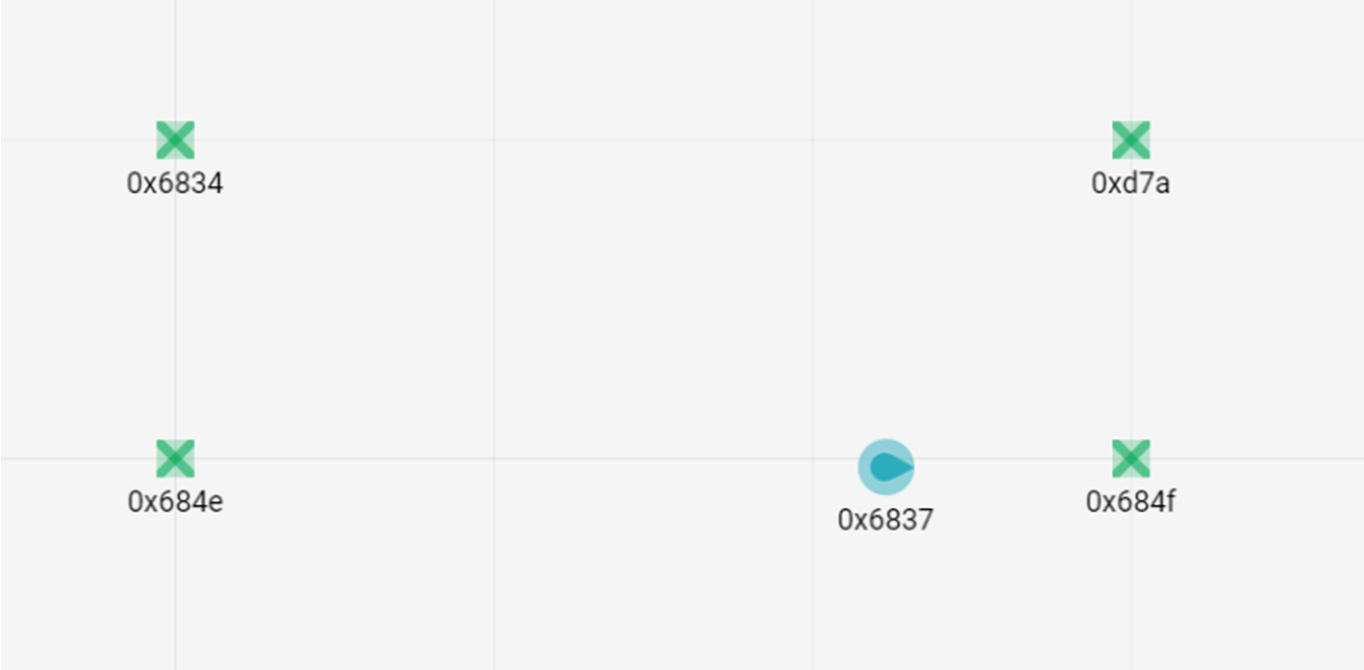
\includegraphics[width=0.5\columnwidth]{figures/creator-controller}
\caption{Pozyx creator controller}
\label{fig:creator-controller}
\end{figure}

\subsection{Avlesning av posisjon med Arduino}
For å kunne bruke dataen fra Pozyx på flightcontrolleren til quadcopteret måtte dataen oversettes til MavLink. 
Til dette ble det brukt en Arduino Nano. Arduinoen ble loddet opp til Pozyx tagen som vist i figur \ref{fig:arduino-tag}.
indoorLoiter (Mackay, 2016), et Arduino program skrevet av Ardupilot, ble brukt på Arduinoen. 
Dette programmet henter data fra Pozyx tagen, oversetter det til MavLink, og sender det deretter ut til Pixhawken.

\begin{figure}[htp]
\centering
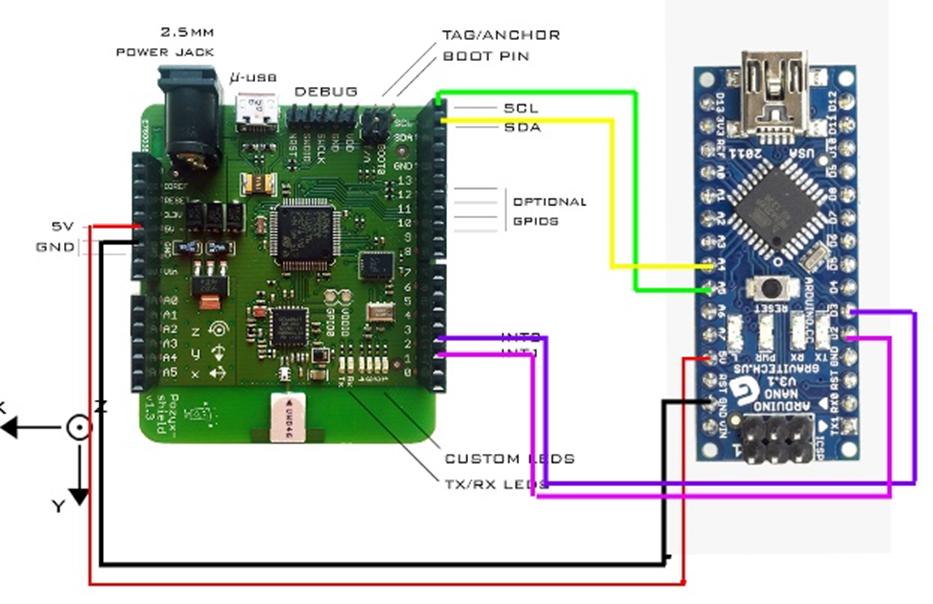
\includegraphics[width=0.5\columnwidth]{figures/oppkobling2}
\caption{Oppkobling av pozyx tag og arduinor}
\label{fig:arduino-tag}
\end{figure}
 
I første omgang ble dette programmet brukt for å teste at Arduinoen faktisk greide å lese av posisjon fra Pozyx tagen, 
og se på nøyaktigheten til systemet.

\subsection{Plotting med python}
Når indoorLoiter programmet kjører på Arduinoen så sender Arduinoen ut posisjonen til tagen i x, y og z retning på USART. 
Dette ble brukt til å lese av posisjonen på en datamaskin som kjørte python, og plotte posisjonen over ulike tidsrom.
Figur \ref{fig:ovenfra} viser et ovenfra plot fra en test der tagen ble beveget rundt i grupperommet. 
Figur \ref{fig:ovenfra} viser et plot fra samme test, men fra siden. 
Plotene viser at posisjonen i x-y retning er mye mer presis enn posisjonen i z retning. 
Det ble ikke gjort mye arbeid for å forbedre dette, da høydeholdet på dronen uansett bruker barometer.

\begin{figure}[htp]
\centering
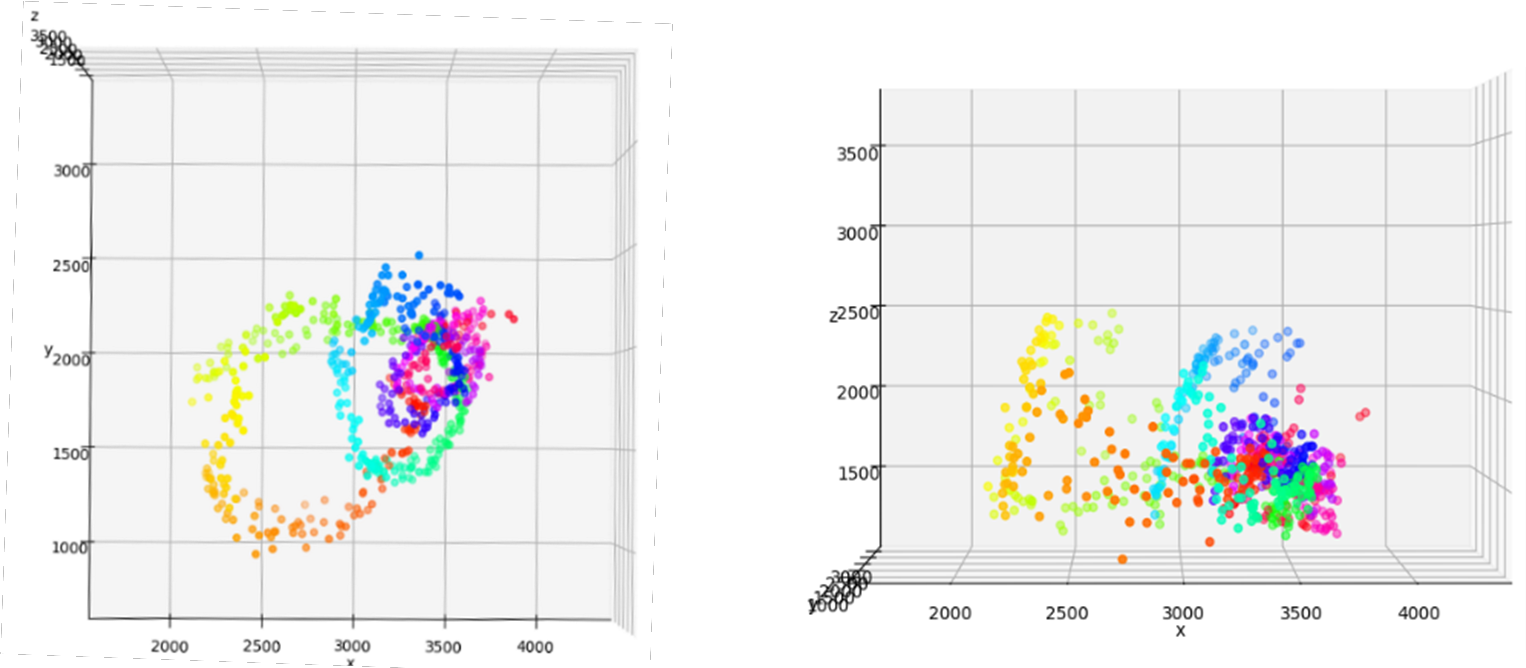
\includegraphics[width=0.5\columnwidth]{figures/plott-ovenfra}
\caption{Plot fra innendørstest. x-y planet i figuren til høyre, x-y planet i figuren til venstre.}
\label{fig:ovenfra}
\end{figure}

\subsection{Presisjon og rekkevidde av UWB system}
Hensikten med denne øvelsen var å teste presisjonen og rekkevidden til UWB systemet. 
Testene ble gjort ute, ved å enten gå rundt med en tag eller la en tag stå festet til en tripod.

\subsubsection{Rekkevidde}
Først ble det utført en test for å se på rekkevidden til systemet. 
RSSI (Received Signal Strength Indicator) ble brukt som en indikator på hvor sterkt signal som ble mottatt, 
og dette ble sammenliknet med avstanden det ble målt over. 
Testen ble gjennomført ved å sette et anker på en tripod, og en tag på en annen tripod. Avstanden mellom disse ble målt opp med målebånd, 
da det var for sterkt lys til å måle opp med laser. De tre første loggingene ble gjennomført på 5 meter, 
og deretter ble tagen flyttet lengre og lengre vekk fra ankeret for vær logging, fem meter om gangen helt opp til 40 meter. 
En logging varte i 20 sekunder, og ga ca. 120 målinger. Figur \ref{fig:RSSI1} viser dataen fra loggene. 
Det øverste plotet viser gjennomsnitts verdien for hver avstand. Det viser en sterk trend på at signalet blir 
svakere når avstanden øker. Plotet under viser at på hver log holder RSSI målingene seg stabilt, med en nøyaktighet på ± 2dBm.

\begin{figure}[htp]
\centering
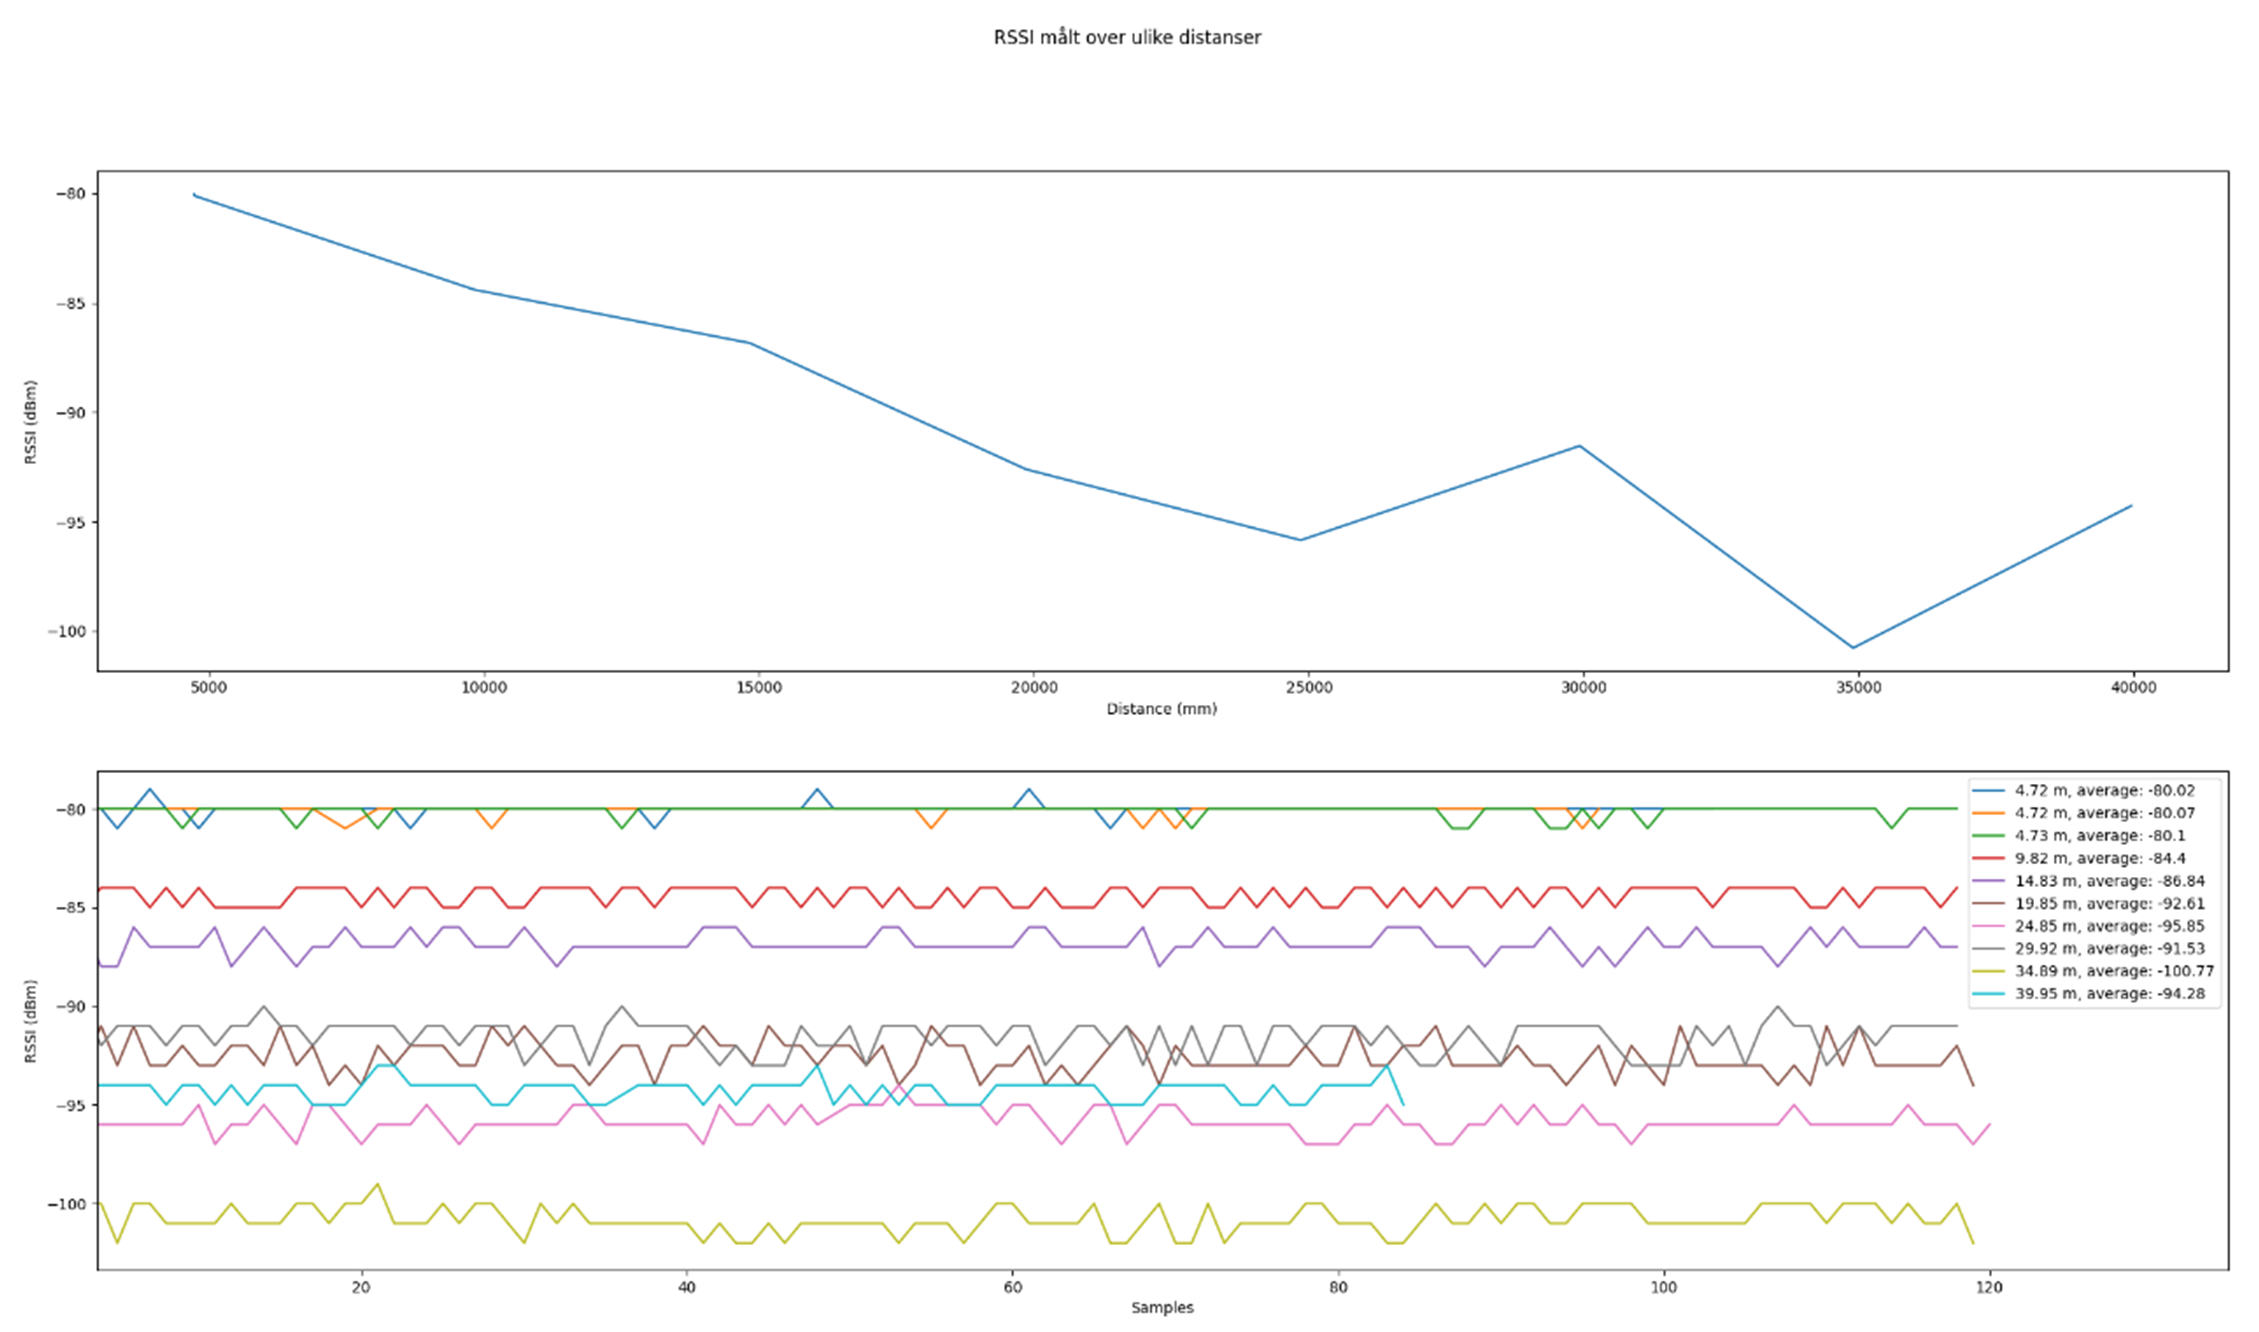
\includegraphics[width=0.5\columnwidth]{figures/rssi-test-ute}
\caption{RSSI måling over ulike distanser.}
\label{fig:RSSI1}
\end{figure}

Det ble også gjennomført en test der tagen ble holdt i hånden, og flyttet fra ca. 5 meter til ca. 80 meter. 
Figur \ref{fig:RSSI2} viser resultatene fra denne testen. Bortsett fra et lite avvik helt i starten av testen, 
så viser dette plotet samme trend som tidligere. RSSI verdiene blir svakere når avstanden øker.

\begin{figure}[htp]
\centering
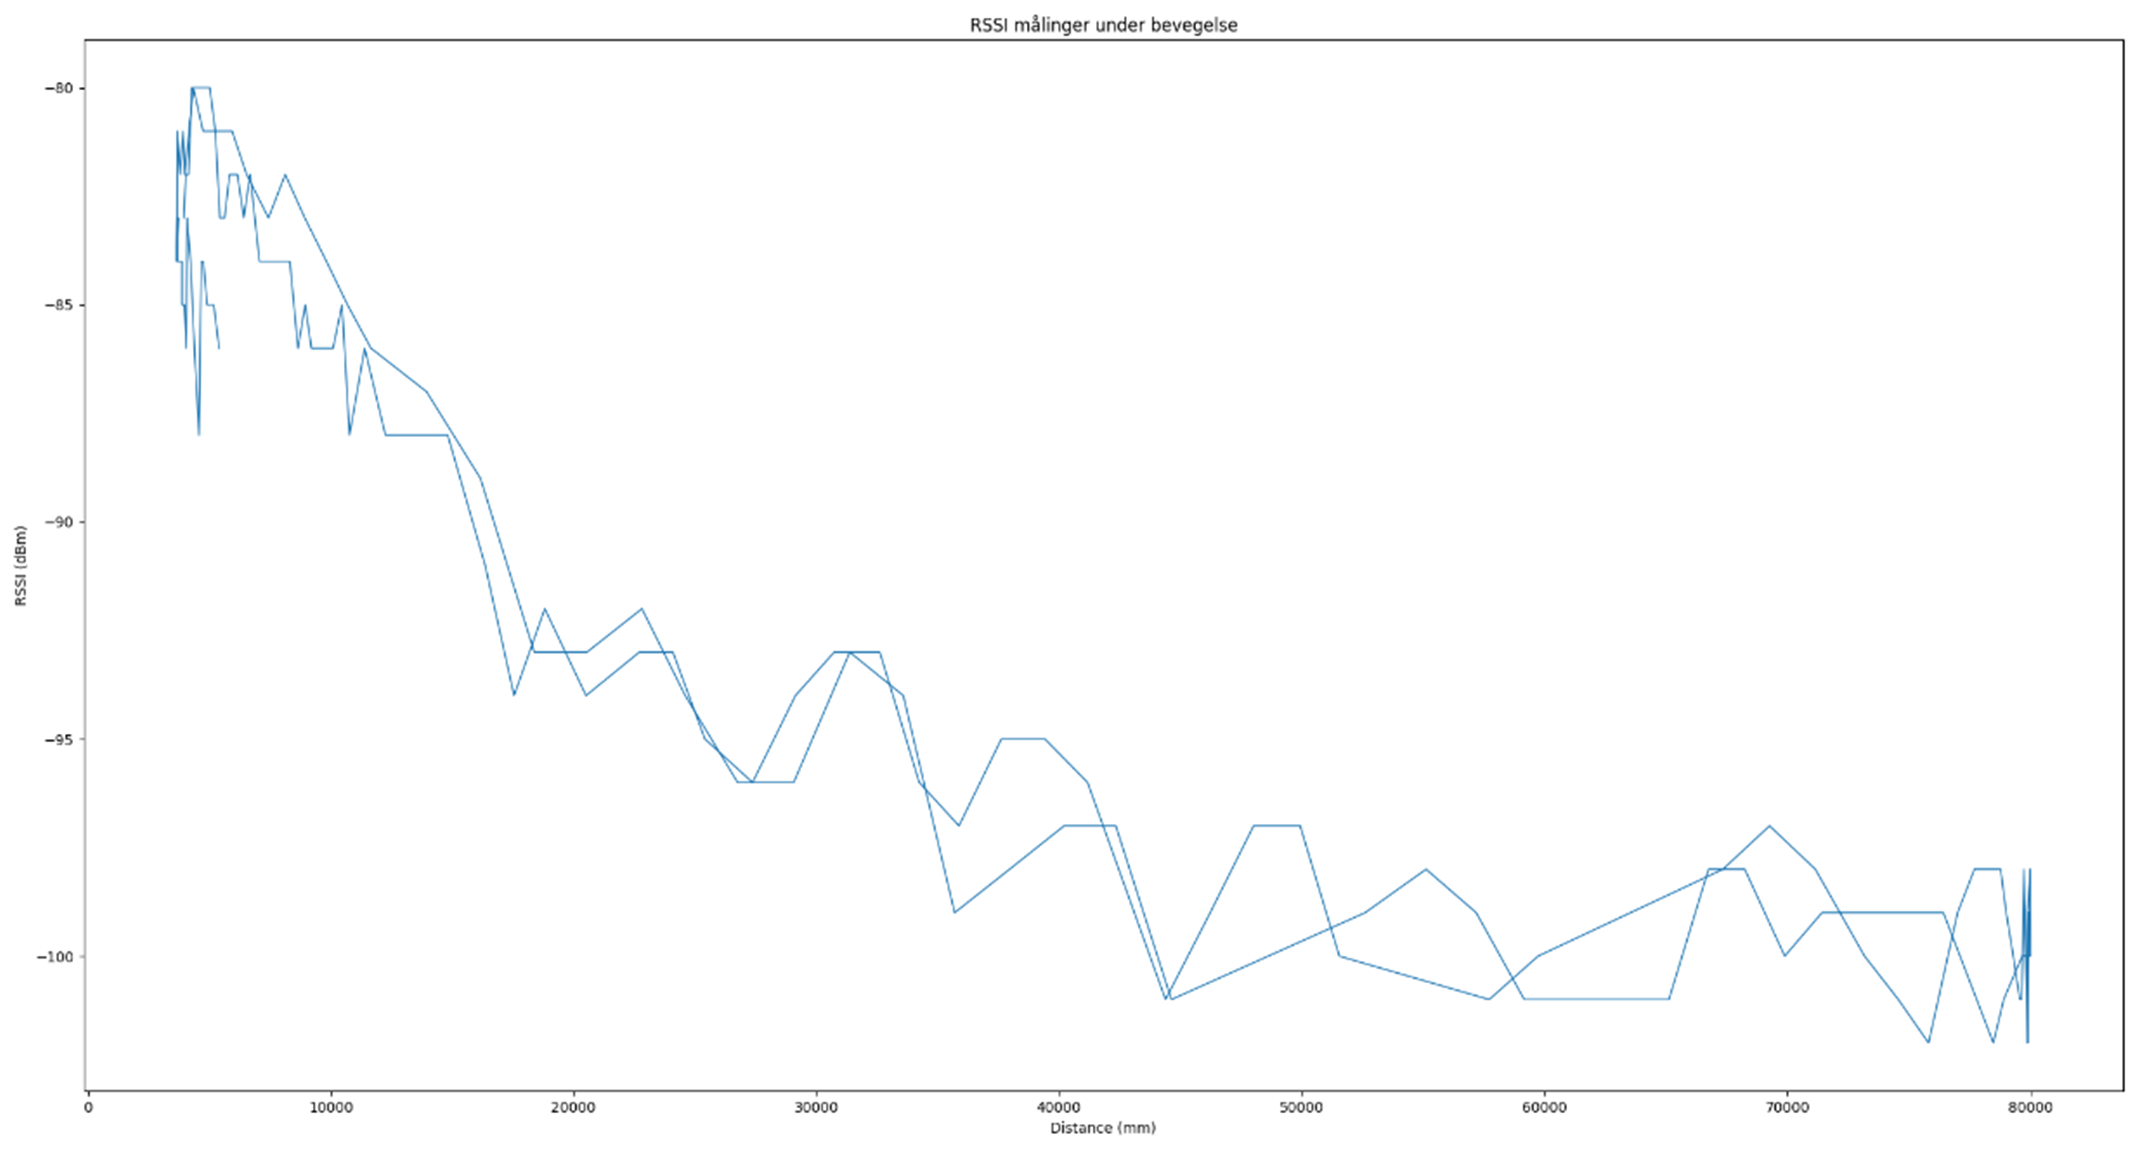
\includegraphics[width=0.5\columnwidth]{figures/rssi-test-ute2}
\caption{RSSI måling over ulike distanser.}
\label{fig:RSSI2}
\end{figure}

\newpage
\subsubsection{Presisjon}
Det ble utført presisjonstester med to ulike anker oppsett. 
De fire første testene ble gjennomført som vist i figur \ref{fig:oppsett}, 
resterende syv tester ble gjennomført slik Figur 15 viser. 
Det ble skrevet et python program for logging av dataen fra Pozyx, 
og et python program for plotting og analyse. 

\begin{figure}[htp]
    \centering
    \subfloat[\centering $2\cdot2 m$]{{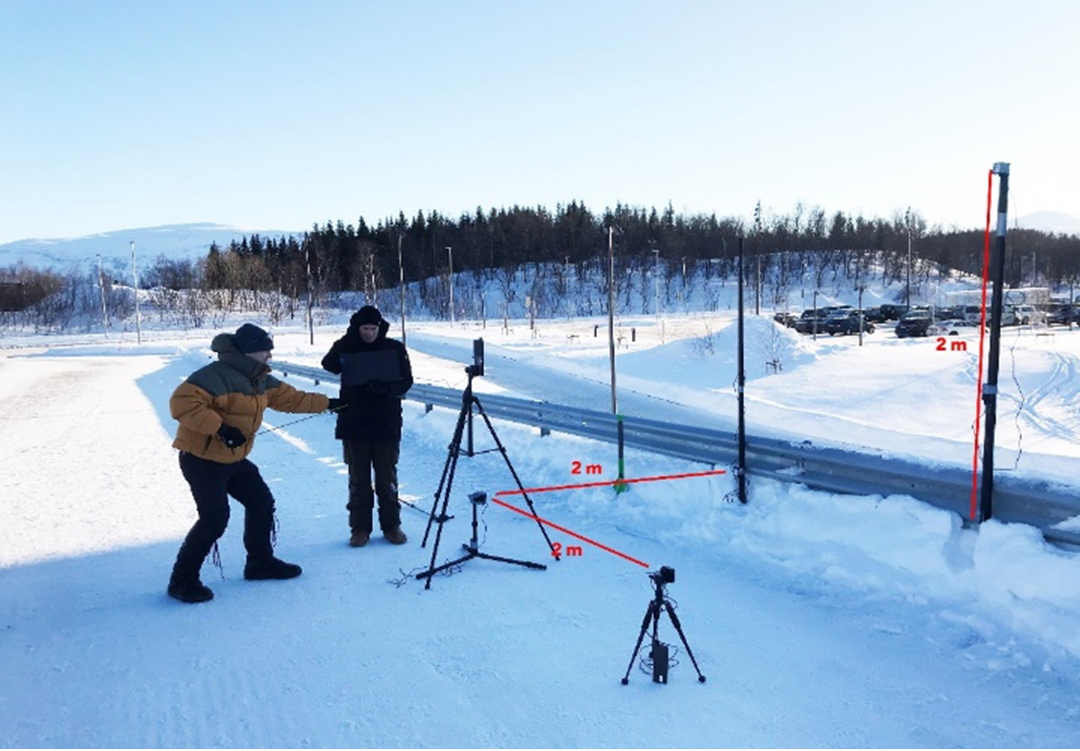
\includegraphics[width=5cm]{figures/ankere2x2} }}%
    \qquad
    \subfloat[\centering $5\cdot5 m$]{{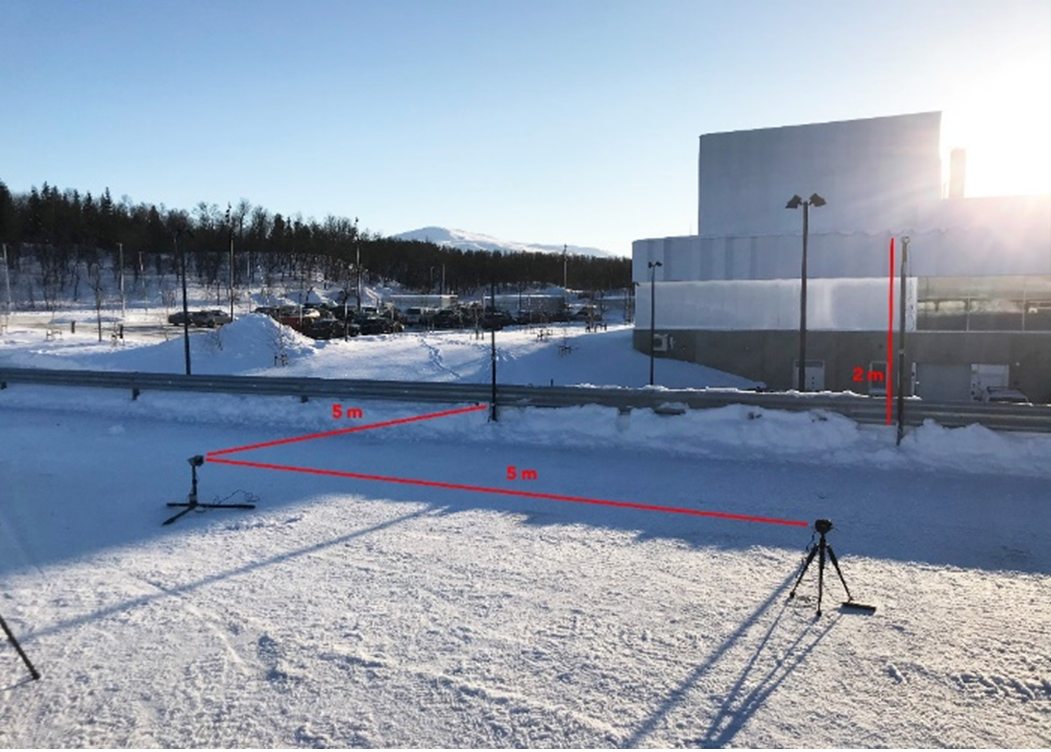
\includegraphics[width=5cm]{figures/ankere5x5} }}%
    \caption{Ulike anker oppsett.}%
    \label{fig:oppsett}%
\end{figure}

Den svarte firkanten i Figur \ref{fig:2x2målinger} og Figur \ref{fig:2x2målinger50} illustrerer 
posisjonen til ankerene i 2x2 meter oppsett, der ankrene er plassert i hvert sitt hjørne. 
Her er målingene plottet etter tid, der det første punktet er lilla og det siste er gult. 

\begin{figure}[htp]
\centering
\includegraphics[width=0.5\columnwidth]{figures/målinger-2x2}
\caption{Målinger med $2\cdot2 m$ ankere.}
\label{fig:2x2målinger}
\end{figure}
\begin{figure}[htp]
\centering
\includegraphics[width=0.5\columnwidth]{figures/målinger-2x2-minus50}
\caption{Målinger med $2\cdot2 m$ ankere uten de 50 første målepunkter.}
\label{fig:2x2målinger50}
\end{figure}

Somf figur \ref{fig:2x2målinger} viser er det mye feilmålinger helt i starten av loggingene. 
I figur \ref{fig:2x2målinger50} er derfor de 50 første målingene fjernet, som omtrent tilsier de første 2 sekundene. 
Tabellene under viser et utdrag fra noen av målingene, med plot og resultater. I utregningene er også de 50 første målingene fjernet.

\begin{figure}[htp]
\centering
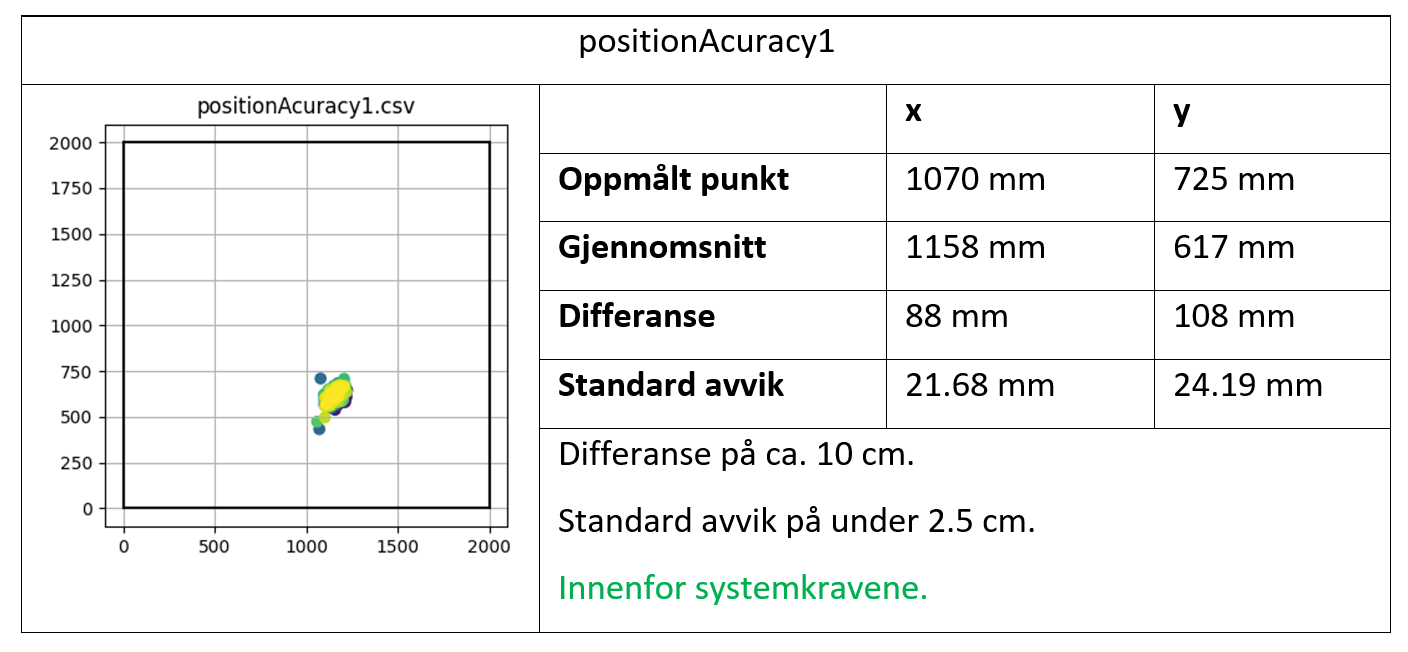
\includegraphics[width=0.5\columnwidth]{figures/2x2resultat1}
\caption{Resultater fra måling 1.}
\label{fig:2x2res1}
\end{figure}
\begin{figure}[htp]
\centering
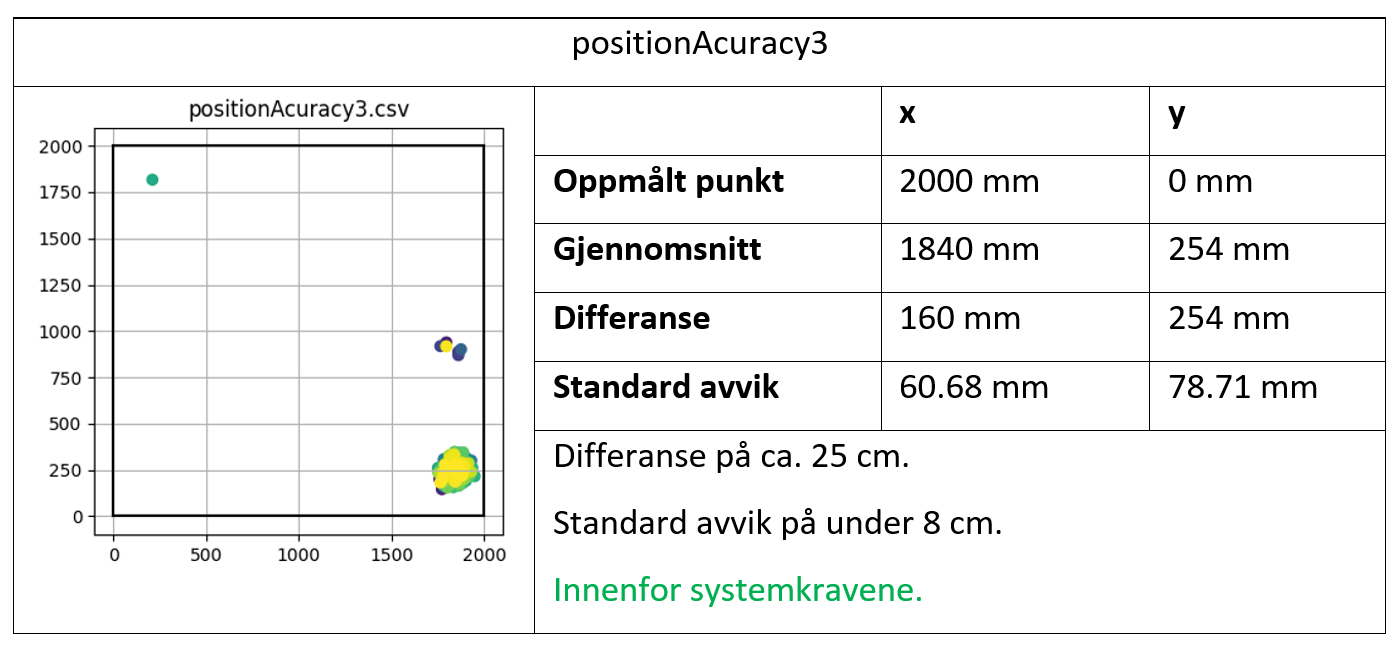
\includegraphics[width=0.5\columnwidth]{figures/2x2resultat3}
\caption{Resultater fra måling 3.}
\label{fig:2x2res3}
\end{figure}
\begin{figure}[htp]
\centering
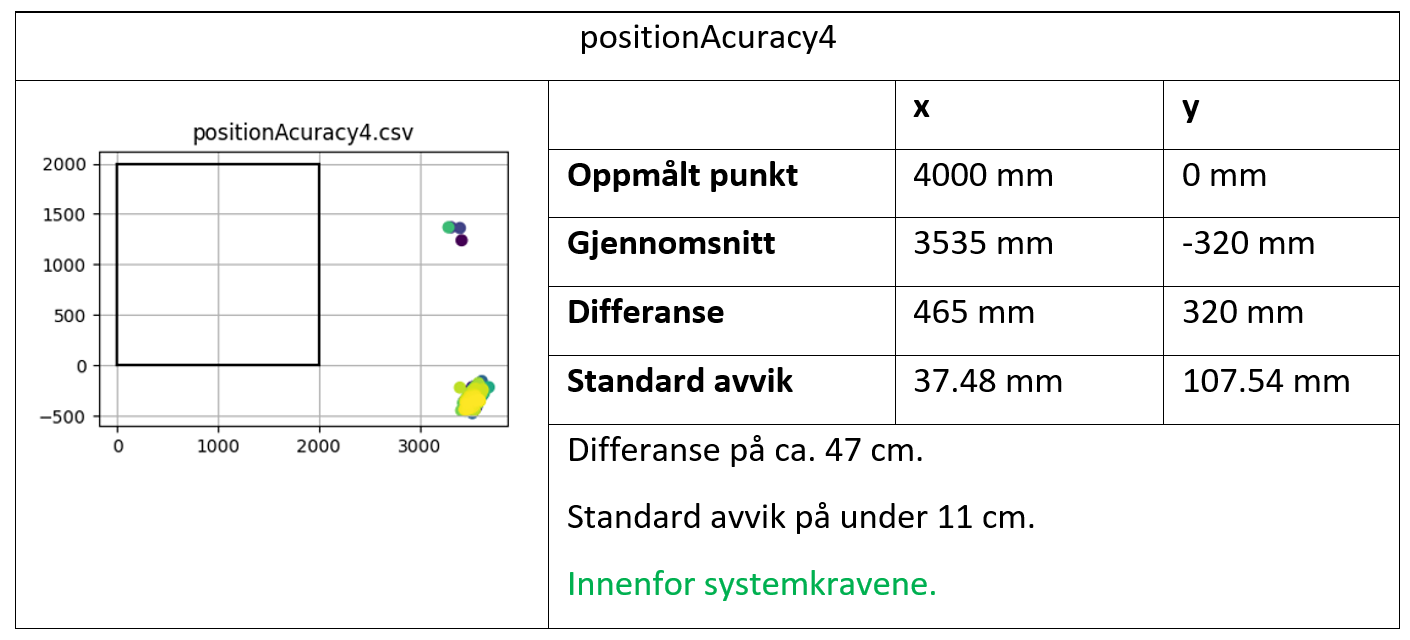
\includegraphics[width=0.5\columnwidth]{figures/2x2resultat4}
\caption{Resultater fra måling 4.}
\label{fig:2x2res4}
\end{figure}

Figur \ref{fig:5x5målinger} og figur \ref{fig:5x5målinger50} viser plot fra logg 6, 7 og 8. 
I figur \ref{fig:5x5målinger50} er de 50 første målingene fjernet for å få bort initialiserings feilmålingene. 

\begin{figure}[htp]
\centering
\includegraphics[width=0.5\columnwidth]{figures/målinger-5x5}
\caption{Målinger med $5\cdot5 m$ ankere.}
\label{fig:5x5målinger}
\end{figure}
\begin{figure}[htp]
\centering
\includegraphics[width=0.5\columnwidth]{figures/målinger-5x5-minus50}
\caption{Målinger med $5\cdot5 m$ ankere uten de 50 første målepunkter.}
\label{fig:5x5målinger50}
\end{figure}

Figur \ref{fig:5x5res6}, {fig:5x5res7} og {fig:5x5res8} under viser de ulike målingene ved 5x5 meter anker oppsett, 
med plot og analyse data.

\begin{figure}[htp]
\centering
\includegraphics[width=0.5\columnwidth]{figures/5x5-resultat6}
\caption{Resultater fra måling 6.}
\label{fig:5x5res6}
\end{figure}
\begin{figure}[htp]
\centering
\includegraphics[width=0.5\columnwidth]{figures/5x5-resultat7}
\caption{Resultater fra måling 7.}
\label{fig:5x5res3}
\end{figure}
\begin{figure}[htp]
\centering
\includegraphics[width=0.5\columnwidth]{figures/5x5-resultat8}
\caption{Resultater fra måling 8.}
\label{fig:5x5res4}
\end{figure}

\newpage
\subsection{Analyse og konklusjon}
Som tabellene for både 2x2 og 5x5 oppsettet viser er det ikke noe merkbar forskjell 
på presisjonene som blir målt. Nøyaktigheten derimot ser ut til å være bedre ved 5x5 oppsettet. 
Der er det største standardavviket på 4.6 cm, mens det for 2x2 er oppe i 11 cm. 
Oppmålingen av anker koordinatene som ble brukt til å regne ut posisjonene er en stor feilkilde i disse testene. 
Bakken der testene ble gjennomført var ikke helt rett, og det var vanskelig å måle nøyaktig med lasermåler på grunn av det sterke sollyset.
Ved å fjerne de 50 første målingene fra testene ble resultantene mye bedre. 
Likevel viser plot 3 og 4 i figur \ref{fig:2x2målinger50} at enda flere målinger burde ha vært fjernet. 
Når systemet brukes for posisjonhold på en drone vil man aldri ta av i løpet av de første sekundene, 
så avviket i initieringsmålingene vil ikke ha noe å si for videre bruk.
Målingene som ble gjort viser at systemet er innenfor kravet om 1m presisjon, og vil derfor kunne brukes videre i prosjektet. 

\subsection{Avlesning av posisjon og oppsett av drone}
Dette kapittelet tar for seg hvordan dronen får posisjon ved hjelp av UWB systemet.
En Pozyx tag, Arduino nano og flightcontroller ble koblet sammen og montert på dronen. 
Pozyx tagen måler avstanden mellom seg og ankerene, og sender disse til Arduinoen. Arduinoen laser av disse avstandene, 
og lager MavLink melinger som vist i figur \ref{fig:melding} slik at Ardupilot kan bruke dataen videre. 
Flightcontrolleren mottar MavLink meldingene, og regner ut posisjonen utafra avstandene til de ulike ankerene. 
Denne kommunikasjonen er illustrert i figur \ref{fig:kommunikasjon}.

\begin{figure}[htp]
\centering
\includegraphics[width=0.5\columnwidth]{figures/melding}
\caption{MavLink melding for anker distanse.}
\label{fig:melding}
\end{figure}

Oppsett av drone:
Det ble utført flere tester av flyvedyktigheten til dronen, etter å fått dronen til å fly var det forbedrigspotensiale i reguleringen. 
Drone fikk osilasjoner som burder bli fikset, men dette måtte bli utført i større lokaler eller utendør når været er bra. 

\begin{figure}[htp]
\centering
\includegraphics[width=0.5\columnwidth]{figures/kommunikasjon}
\caption{Kommunikasjons vei for tag, arduino og flightcontroller.}
\label{fig:kommunikasjon}
\end{figure}

\subsection{Test av posisjonshold i gang}
Etter å ha fått posisjon estimat i dronen under flyvning, var det neste steget å få dronen til å holde posisjon i luften. 

\subsection{Test av presisjon i krafthallen}
For å få mindre magnetisk forstyrrelse og kunne tune drone bedre, ble det planlagt å fly i krafthallen. 
Autotune, for liten flytid. 

\subsection{Test av posisjonhold I Hamnahallen}
Pid-regulering. 
Loiter test

\subsection{Test av automatisk landing og preprogrammert rute}
Fra tidligere tester hadde dronen suksessfullt klart å holde posisjonen i luften. 
Dronen fløy godt med nye PID-verdier. Vider i planen stod det å teste automatisk landing og flyging med preprogrammert rute. 
Testene ble utført i den eldre gymsalen på kraftsportsenter. 
Der var ankerene satt opp som hamnahallen med 12x12m oppsett i 150cm høyde. 
Før testing ble utført ble oppsettet testet etter sjekklisten. 
Når dronen var koblet opp mot basestasjonen ble dronen bevegd rundt i rommet for å se om posisjonen endret seg riktig. 
En testflight i posisjonhold ble utført for å se om det var noen problem med drone eller posisjonsystemet.  

\subsubsection{Landing}
Dronen ble satt til å lande på en landingspad for å kunne gi indikasjon på treffsikkerheten til systemet. Landingspadden har en diameter på 100cm. 



%----------------------------------------------------------------------------------------
%	BIBLIOGRAPHY
%----------------------------------------------------------------------------------------
\newpage
\renewcommand{\refname}{\spacedlowsmallcaps{References}} % For modifying the bibliography heading

%\bibliographystyle{unsrt}

%\bibliography{kilder.bib} % The file containing the bibliography

\printbibliography

%----------------------------------------------------------------------------------------
\end{sloppypar}

\end{document}